\pdfbookmark{Общая характеристика работы}{characteristic}             % Закладка pdf
\section*{Общая характеристика работы}

\newcommand{\actuality}{\pdfbookmark[1]{Актуальность}{actuality}\underline{\textbf{\actualityTXT}}}
\newcommand{\progress}{\pdfbookmark[1]{Разработанность темы}{progress}\underline{\textbf{\progressTXT}}}
\newcommand{\aim}{\pdfbookmark[1]{Цели}{aim}\underline{{\textbf\aimTXT}}}
\newcommand{\object}{\pdfbookmark[1]{Объект и предмет исследования}{object}\underline{{\textbf\objectTXT}}}
\newcommand{\tasks}{\pdfbookmark[1]{Задачи}{tasks}\underline{\textbf{\tasksTXT}}}
\newcommand{\aimtasks}{\pdfbookmark[1]{Цели и задачи}{aimtasks}\aimtasksTXT}
\newcommand{\novelty}{\pdfbookmark[1]{Научная новизна}{novelty}\underline{\textbf{\noveltyTXT}}}
\newcommand{\influence}{\pdfbookmark[1]{Практическая значимость}{influence}\underline{\textbf{\influenceTXT}}}
\newcommand{\methods}{\pdfbookmark[1]{Методология и методы исследования}{methods}\underline{\textbf{\methodsTXT}}}
\newcommand{\defpositions}{\pdfbookmark[1]{Положения, выносимые на защиту}{defpositions}\underline{\textbf{\defpositionsTXT}}}
\newcommand{\reliability}{\pdfbookmark[1]{Достоверность}{reliability}\underline{\textbf{\reliabilityTXT}}}
\newcommand{\probation}{\pdfbookmark[1]{Апробация}{probation}\underline{\textbf{\probationTXT}}}
\newcommand{\contribution}{\pdfbookmark[1]{Личный вклад}{contribution}\underline{\textbf{\contributionTXT}}}
\newcommand{\publications}{\pdfbookmark[1]{Публикации}{publications}\underline{\textbf{\publicationsTXT}}}
\newcommand{\acknowledge}{\pdfbookmark[1]{Благодарности}{acknowledge}\underline{\textbf{\acknowledgeTXT}}}

{\actuality}
%\ifdefined\DISSER
%Понимание механизмов функционирования живых систем на молекулярном и надмолекулярном (супрамолекулярном) уровнях является одной из ключевых задач биологии XXI века. Такое понимание важно не только с фундаментальной точки зрения, но и имеет прямые практические приложения в области медицины, здравоохранения, биоинженерии и биотехнологии. Значение термина ``понимание'' в этой связи хорошо проиллюстрировать цитатой Р. Фейнмана ``То, чего я не могу сделать - я не понимаю''\footnote{Англ. What I cannot create - I do not understand.}. Ключевой областью науки, способствующей пониманию работы живых систем на молекулярном уровне, является направление \textit{структурной биологии}. Работы середины XX века Д. Уотсона, Ф. Крика, М. Уилкинса, Р. Франклин, М. Перутца, Д. Кендрю заложили основы нашего понимания устройства ДНК и белков на атомистическом уровне и дали толчок развитию структурной и молекулярной биологии, биохимии на долгие годы вперед. Методы рентгеноструктурного анализа, биомолекулярной ЯМР-спектроскопии, электронной дифракции и микроскопии позволили определить по состоянию на 2020 год более 150 тысяч структур различных макромолекул и их комплексов\footnote{\url{https://www.rcsb.org/stats}}. На основе данной структурной информации были расшифрованы многие ключевые механизмы работы биологических систем.

%Со временем, однако, стали понятны и ограничения классических методов структурной биологии в изучении структуры и механизмов работы биомакромолекул и их комплексов. Можно выделить три типа ограничений. Во-первых, это ограничения, связанные с динамикой исследуемых биомолекул. Наличие различных конформаций биологического объекта приводит к тому, что определить его структуру, а также структуру различных конформаций становится значительно сложнее. Динамика объекта с одной стороны мешает пробоподготовке (например, кристаллизации в методах РСА), с другой ухудшает разрешение получаемой структурной модели, которая во многих случаях будет уже описывать некоторое усредненное конформационное состояние. Во-вторых, методы структурной биологии с трудом применимы к большим биомакромолекулярным комплексам -- по состоянию на 2020 год 92\% структур депонированные в базе PDB\footnote{\url{https://www.rcsb.org/stats/distribution-molecular-weight-entity}} имеют молекулярный вес менее 75 кДа, тогда как небольшой биомакромолекулярный комплекс, нуклеосома, имеет молекулярный вес около 200 кДа. Данный факт связан опять же с трудностью пробоподготовки больших структур и наличием крупномасштабных динамических мод. В-третьих, по мере увеличения размеров биомакромолекулярных комплексов механизмы их работы становятся все более сложными, связанными с переходами между многими конформационными состояниями, на вероятность которых влияют различные факторы физической и химической природы. Таким образом, становится все сложнее делать выводы о механизмах функционирования биомакромолекулярных комплексов, даже если удается разрешить их структуру. 

%Весьма характерным примером в этом плане является история изучения хроматина в эукариотических клетках. С момента открытия нуклеосом (определения их состава и наблюдения методами электронной микроскопии) в 1974 году \cite{kornberg_chromatin_1974-1,olins_spheroid_1974} потребовалось более 20 лет, чтобы определить детальную структурную организацию нуклеосом методами РСА \cite{luger_crystal_1997}. Попытки установить структуры комплексов нуклеосом с белками хроматина долгое время не увенчивались успехом. Так, чтобы получить структуру нуклеосомы с  небольшим белком, гистоном H1, ушло еще около 20 лет \cite{zhou_structural_2015}. В последнее время, благодаря успехам криоэлектронной микроскопии, удается разрешать структуры нуклеосом с более крупными комплексами белков хроматина, например, комплексами ремоделирвоания нуклеосом \cite{willhoft_structure_2018}. Однако из-за их динамичности, в том числе полиморфизма структры и меняющегося состава субъединиц, механизмы их функционирования и регуляции остаются плохо понятными. На более крупных масштабах организации хроматина динамичность взаимодействий проявляется еще сильнее. В настоящее время популярной является гипотеза, согласно которой в структурной организации хроматина важную роль играют физические и статистические эффекты, свойственные мягкой материи (soft matter). Например, эффекты фазового разделения между жидкими каплями различного состава и свойства (liquid-liquid phase separation) \cite{zhang_liquidliquid_2019}. Традиционно используемые в структурной биологии подходы представления структурной информации в принципе плохо применимы к описанию такого рода эффектов структурирования биологической материи.

%В задачах изучения механизмов биологических процессов важным дополнением к экспериментальным методам структурной биологии служат методы компьютерного молекулярного моделирования, которые позволяют рассчитывать свойства биомакромолекул на основе моделей физических взаимодействий между отдельными атомами или группами атомов. Для моделирования биологических молекул данные методы активно развиваются с начала 1980-ых годов. В качестве примера успешного взаимодополнения методов структурной биологии и компьютерного моделирования можно привести первые работы по моделированию связывания кислорода с миоглобином \cite{case_dynamic_1986}. Взрывной рост возможностей компьютерных вычислений, в том числе суперкомпьютерных, в последние десятилетия привел к серьезному прогрессу в области компьютерного молекулярного моделирования. Стало возможным моделирование систем состоящих из сотен тысяч и миллионов атомов (частиц) на временах десятков микросекунд, а с использованием специализированных суперкомпьютеров и на миллисекундных временах. Стало возможным моделирование фолднига небольших белков, наблюдения переключения белков между различными конформационными состояниями в ответ на внешнее воздействие \textit{in silico} \cite{jensen_mechanism_2012}.  Однако, присутствуют и существенные ограничения в области применения методов компьютерного моделирования для изучения биомолекулярных систем. Во-первых, это ограничения связанные с ограниченной возможность по изучению временной эволюции моделируемых систем. Многие физиологически важные процессы на супрамолекулярном уровне (например, динамика и ремоделирование нуклеосом) зачастую находятся в субсекундном и секундном диапазоне времен, тогда как методы моделирования пока в лучшем случае позволяют просчитывать динамику в микросекундном диапазоне. Второе ограничение связано с качеством параметризации атом-атомных взаимодействий, так называемых силовых полей. Несмотря на значительные успехи в этой области, возможность моделировать процессы фолдинга белков, а в некоторых случаях, предсказывать белковые структуры \textit{ab initio}, качество силовых полей не позволяет точно решать многие задачи, связанные  с правильным учетом вероятностного/энергетического баланса между различными конформациями биомакромолекул. Известно, что современные силовые поля испытывают затруднения при описании неструктурированных белков (intrinsically disordered proteins), а для глобулярных белков модели нативного состояния оказываются чрезмерно стабильными, переоценивающими гидрофобные эффекты \cite{shaytan_free_2010,petrov_are_2014}.

%Таким образом, весьма актуальной остается проблема построения и изучения структурно-динамических моделей биомакромолекулярных комплексов, в особенности в интервале размеров и динамических времен, не поддающихся прямой характеризации методами классической структурной биологии. Для интервала времен и размеров молекулярных систем, поддающихся описанию методами атомистического молекулярного моделирования, актуальными остаются проблемы сопряжения результатов расчета с непосредственно измеримыми в экспериментах параметрами. Развитию подходов, нацеленных на решение вышеозначенных проблем, и их применению для ряда биомакромолекулярных систем посвящена настоящая диссертационная работа. При построении структурно-динамических моделей биомакромолекулярных комплексов актуальным также является использование не только экспериментальных данных высокой детальности и информационного содержания (получаемых методами РСА, ЯМР, криоЭМ), которые могут быть доступны в ограниченном объеме, но и различных экспериментальных данных низкого информационного содержания, получаемых в ходе биофизических, биохимических, функциональных, спектроскопических и других экспериментов. Для названия подходов, основанных на интеграции различных экспериментальных данных для построения структурно-динамических моделей, будем использовать термин \textit{интегративное моделирование}, следуя практике использования данного термина в англоязычной литературе \cite{braitbard_integrative_2019}. В данной диссертационной работе методы интегративного моделирования разрабатывались и применялись, в том числе для создания молекулярных моделей нуклеосом, комплексов нуклеосом с белками хроматина, амилоидоподобных фибрилл. Актуальность исследования нуклеосом и их комплексов напрямую связана с необходимостью понимания функционирования хроматина в клетках эукариотических организмов, что в свою очередь необходимо для понимания функционирования и развития живых организмов. Актуальность исследования амилоидоподобных фибрилл связана с их вовлеченностью в ряд биологических процессов, в том числе патологических, а также с возможностью использования эффектов самосборки пептидов в амилоидоподобные фибриллы для создания функциональных нанотехнологических и биотехнологических конструкций.
%\else
Понимание механизмов функционирования живых систем на молекулярном и супрамолекулярном уровнях является одной из ключевых задач биологии XXI века. Такое понимание важно не только с фундаментальной точки зрения, но и имеет прямые практические приложения в области медицины, здравоохранения, биоинженерии и биотехнологии. 
Особенностью биологических молекул является формирование ими сложных пространственных структур, которые могут перестраиваться в ходе различных функциональных процессов.
Исследование \textit{структурно-динамических} моделей биомакромолекул является одним из ключевых подходов к изучению механизмов функционирования живой материи.
Методы компьютерного молекулярного моделирования являются неотъемлемой частью этого подхода. Среди методов построения моделей важное место занимают методы, использующие экспериментальные данные рентгеноструктурного анализа (РСА), ядерно-магнитного резонанса (ЯМР), криоэлектронной микроскопии (криоЭМ). В настоящее время они сочетаются с методами молекулярной динамики (МД), Монте-Карло, позволяющих проводить \textit{компьютерные эксперименты}, имитационное моделирование молекулярных систем. В этой области существуют и ограничения, которые затрудняют исследования биологический систем значительных размеров таких, как большинство биомакромолекулярных комплексов. Сложность инетерпретации и самого получения данных РСА, ЯМР, криоЭМ возрастает по мере увеличения размера и конформационной подвижности исследуемой системы. По состоянию на 2020 год 92\% структур депонированные в базе PDB имеют молекулярный вес менее 75 кДа. Возможности исследования больших биомакромолекулярных комплексов (от 100 кДа и более) методами молекулярной динамики ограничиваются вычислительными возможностями и качеством параметризации атом-атомных взаимодействий (так называемых силовых полей). Несмотря на то, что благодаря прогрессу компьютерных технологий, методом МД стал возможен расчет систем, состоящих из сотен тысяч и миллионов атомов на временах десятков микросекунд (а с использованием специализированных суперкомпьютеров и на миллисекундных временах), временные масштабы многих физиологически важных процессов, включая важные моды динамики многих биомакромолекулярных комплексов, находятся пока за пределами возможностей моделирования в субсекундном и секундном диапазоне времен.  С ростом размера биомолекулярной системы неточности задания атом-атомных взаимодействий суммируются и сильнее отражаются на качестве воспроизведения ее динамики, в то время как количество динамических состояний увеличивается, а разница свободной энергии между ними уменьшается.
\textit{Преодоление вышеописанных ограничений с целью построения и анализа структурно-динамических моделей биомакромолекулярных комплексов является важной задачей.}
На современном этапе одним из основных путей решения данной задачи является разработка и совершенствование подходов, которые используют для построения моделей как расчет физических взаимодействий между атомами, так и различные экспериментальные данные. К таким экспериментальным данным могут относится как данные классических методов структурной биологии (данные РСА, ЯМР, криоЭМ), так и данные спектральных методов, различных видов микроскопии, биохимического анализа. 
%Методы работы с последним типом данных, например, расстояниями между молекулярными группами, вероятностью их взаимодействия с химическими агентами, формой молекулярного комплекса особенно актуальны ввиду относительной простоты их экспериментального получения.
%С развитием вычислительных технологий важное значение приобрели методы компьютерного молекулярного моделирования. Данные методы могут быть использованы, как для эффективной интерпретации экспериментальных данных, так и для расчетов структуры и динамики биомолекул на основе моделей физических взаимодействий между атомами. К последнему классу методов, относятся \textit{компьютерные эксперименты} на основе метода молекулярной динамики (МД).
%В настоящее время методом МД стал возможен расчет систем состоящих из сотен тысяч и миллионов атомов на временах десятков микросекунд, а с использованием специализированных суперкомпьютеров и на миллисекундных временах. Однако, в этой области также присутствуют существенные ограничения. Во-первых, временные масштабы многих физиологически важных процессов, включая важные моды динамики многих биомакромолекулярных комплексов, находятся за пределами возможностей моделирования в субсекундном и секундном диапазоне времен. Второе ограничение связано с качеством параметризации атом-атомных взаимодействий, так называемых, силовых полей. С ростом размера молекулярной системы неточность задания силовых полей обычно сильнее сказывается на качестве структурно-динамической модели.

%\fi

%степень разработанности темы исследования
{\progress} 
%\ifdefined\DISSER
%Обсуждение степени разработанности темы исследований структурировано ниже следующим образом - в начале обсуждается степень разработанности темы компьютерного молекулярного моделирования в целом, затем степень разработанности методов интегративного моделирования, далее обсуждаются степень разработанности конкретных тем, освещенных в диссертации по следующему плану: моделирование нуклеосом методом молекулярной динамики, моделирование на основе данных по расщеплению ДНК гидроксильными радикалами, интегративное моделирование комплексов нуклеосом и белков хроматина, моделирование амилоидоподобных фибрилл.

%Методы компьютерного молекулярного моделирования активно развиваются с середины 1940-годов и по настоящее время. Как отмечалось выше, достигнут существенный прогресс в возможностях моделирования биологических систем размерами в сотни тысяч и миллионы атомов на временах до десятков микросекунд и даже миллисекунд. Основными стратегическими направлениями дальнейших работ является увеличение доступных времен моделирования, благодаря совершенствованию программных и аппаратных технологий, а также совершенствование силовых полей для максимально реалистичной параметризации моделей биомакромолекул.

%Интегративное моделирование является достаточно широким классом методов и подходов. Задачи поиска структуры биомолекул, отвечающих заданным экспериментальным данным, решаются, в том числе и при построении моделей методами РСА, криоЭМ, ЯМР, но для определенного класса экспериментальных данных. Если в случае РСА и криоЭМ построение моделей может зачастую производится вручную путем вписывания координат атомов в электронную плотность, то интерпретация данных ЯМР уже требует компьютерных алгоритмов оптимизации структуры на основе более косвенных экспериментальных данных, например, расстояний между атомами. Поэтому программы используемые для реконструкции структур по данным ЯМР, вероятно, первыми начали включать в себя функциональность по использованию некоторых типов данных из других экспериментов, например, данных малоуглового рентгеновского и нейтронного рассеяния  \cite{schwieters_xplor-nih_2003}. Похожие методы оптимизации решаются при построении моделей белков по гомологии  \cite{sali_comparative_1993}. Существуют разработки по использованию карт электронной плотности низкого разрешения для направления структурных деформаций биомолекул при расчетах методами молекулярной динамики и оптимизационного моделирования \cite{mcgreevy_xmdff_2014,wriggers_conventions_2012}. Некоторыми группами разрабатываются программные платформы для более системного подхода к интегративному моделированию биомолекул с учетом данных различных биофизических и биохимических экспериментов \cite{russel_putting_2012}. Следует однако отметить, что в отличие от подходов атомистической молекулярной динамики, подходы интегративного моделирования являются достаточно разнообразными и зачастую заточены под моделирование определенного класса систем с использованием определенного класса экспериментальных данных. Их систематизацию можно проводить по крайней мере по трем характеристиками - (i) уровню представления модели (напр. атомистическое, огрубленное), (ii) способу оценки соответствия модели экспериментальным данным, включая возможное задание скоринговой функции, (iii) методам поиска структуры, соответствующей экспериментальным данным, включая алгоритмы оптимизации и задания варьируемых параметров. В этом плане имеющиеся программные продукты и платформы пока далеки от универсальности.

%Моделирование нуклеосом методами молекулярной динамики является достаточно активной темой исследований, количество публикаций по которой растет и приближается к сотне\footnote{Запрос к PubMed <<``molecular dynamics simulations'' nucleosome>> выдает 86 записей на момент написания диссертации.}. По мере роста производительности вычислительных ресурсов открываются новые возможности по исследованию динамики нуклеосом на все больших временах. В 2016 году нами были опубликованы результаты по микросекундному моделированию, в данной работе приведены уже результаты по моделированию на временах превышающих 10 микросекунд.

%%Оценка термодинамических параметров гидратации малых молекул с высокой точностью путем прямых расчетов методом молекулярной динамики в явном растворителе стала возможной в начале XXI века благодаря прогрессу в скорости вычислений и развитию методов так называемой вычислительной алхимии (расчетов систем с гамильтонианом взаимодействий между частями, зависящим от варьируемого параметра). С тех пор по этой теме было опубликовано достаточно много работ, однако, исследователями рассматривалась гидратация в объеме растворителя, а не вблизи поверхности воды.


%Методы футпринтинга ДНК гидроксильными радикалами развиваются с конца 1980-ых годов \cite{churchill_detection_1990}. Существенный вклад в понимание механизмов расщепления ДНК был внесен группой Т. Туллиуса \cite{balasubramanian_dna_1998}. Этой же группой были заложены основы цифровой обработки данных футпринтинга, реализованной в ряде программ \cite{shadle_quantitative_1997,das_safa_2005}. Однако по состоянию на середину второй декады XXI века программные разработанные ранее программные инструменты не поддерживались разработчиками, и их использование было серьезно затруднено, особенно с целью интеграции получаемых данных в комплексные пайплайны обработки, визуализации и моделирования.

%Интегративное моделирование структуры комплексов нуклеосом с белками хроматина долгое время было затруднительным из-за отсутствия структуры нуклеосомы высокого разрешения, которая была получена в 1997 году \cite{luger_crystal_1997}. Следующим важным шагом, упрощающим построение таких моделей, явились разработки методов описания конформации ДНК в пространстве координат взаимного расположения азотистых оснований с возможностью перехода из огрубленного приближения в атомистическое и оценкой энергии изгиба ДНК \cite{olson_dna_1998,lu_3dna_2003}. На данный момент возможности построения и анализа интегративных моделей нуклеосом с белками хроматина ограничены в основном доступностью качественных экспериментальных данных.

%Тема изучения амилоидоподобных фибрилл является весьма популярной тематикой исследований, в том числе методами молекулярного моделирования \cite{lu_understanding_2018}. Благодаря вовлеченности процессов амилоидизации в ряд болезней человека, существенная часть работ посвящена изучению определенных типов фибрилл, в частности фибрилл формируемых амилоидом $\beta$. Для фибрилл, представляющих чрезвычайный медицинский интерес, доступно большое количество экспериментальных данных, в том числе методами ЯМР, РСА \cite{sawaya_atomic_2007}.  Исследования других типов фибрилл являются не настолько активными, для них доступно меньше экспериментальных данных и актуальными являются подходы интегративного моделирования.


%\else
Методы молекулярного компьютерного моделирования зародились в 1940-ых годах с появлением первых вычислительных систем, однако активное их применение к биологическим молекулам стало возможным в 1970-ых -- 1980-ых годах. Активно стали развиваться как подходы к моделированию биомолекул методом МД, так и оптимизационные методы моделирования структуры на основе экспериментальных данных (главным образом РСА и ЯМР). Методы МД основаны на представлении молекулярной системы в виде набора атомов, взаимодействующих согласно законам классической механики Ньютона, и численном решении уравнений движения. На сегодняшний день разработана обширная методическая база для моделирования белков, нуклеиновых кислот, липидов методами молекулярной динамики, разработаны наборы функциональных форм и параметров, описывающих взаимодействия между атомами (например, семейства силовых полей CHARMM, AMBER, OPLS и др.), алгоритмы численного интегрирования уравнений движения, поддержания температуры, давления, использования параллельных суперкомпьютерных технологий, созданы программные комплексы для расчетов (например, AMBER, CHARMM, GROMACS, NAMD, PUMA и др.).
В то же время уровень развития методов МД, как с точки зрения доступных времен моделирования, так и с точки зрения качества силовых полей, не позволяет использовать их полностью независимым образом в отрыве от экспериментальных данных. Стандартной практикой для расчетов методом МД является использование в качестве стартовой конформации биомакромолекулярной системы структурной модели, полученной на основе данных РСА, ЯМР, криоЭМ. 
%В случае, если такая модель отсутвует, применение методов МД становится практически невозможным. Зачастую, такая ситуация возникает при изучении биомакромолекулярных комплексов. 

Важный вклад в построение структурных моделей биомакромолекулярных системы вносят комбинированные вычислительные подходы, которые, кроме данных РСА, ЯМР, криоЭМ, могут использовать различные экспериментальные данные, получаемые в ходе биофизических, биохимических, функциональных, спектроскопических и других экспериментов. Такого рода эксперименты могут предоставлять информацию о расстояниях между введенными метками в белке или ДНК (например, методы FRET, ЭПР), характере укладки белковой цепи (например, ИК-, КД-спектроскопия, дифракция рентгеновских лучей на фибриллах), реакционной доступности химических групп (методы футпринтинга, химического сшивания) и др. Такой подход, основанный на интеграции различных экспериментальных данных при построении структурно-динамических моделей, в литературе называется \textit{интегративным моделированием} \cite{braitbard_integrative_2019}\footnote{Ссылки на список литературы приведены цифрами, ссылки на список статей автора -- цифрами \ifdefined\DISSER с буквой A. \else со звездочкой.\fi}. Программы, используемые для реконструкции структур по данным экспериментов ЯМР, вероятно, первыми начали позволять использовать некоторые типы данных из других экспериментов, например, данные малоуглового рентгеновского и нейтронного рассеяния  \cite{schwieters_xplor-nih_2003}. Другим примером является использование в методах МД дополнительных членов потенциальной энергии, которые зависят от экспериментально полученных карт электронной плотности низкого разрешения методами электронной микроскопии или РСА. Такой подход позволят деформировать начальные структуры биомолекул для придания им экспериментально наблюдаемой формы \cite{mcgreevy_xmdff_2014}. Разрабатываются программные подходы, предоставляющие возможность одновременно использовать данные различных биофизических и биохимических экспериментов (например, карты электронной плотности и расстояния между группами атомов) \cite{russel_putting_2012}. В целом подходы интегративного моделирования могут различаться по (i) уровню представления модели (например, атомистическое или огрубленное представление модели), (ii) способу оценки соответствия модели экспериментальным данным (использование различных силовых полей или оценочных функций), (iii) методам поиска структуры, соответствующей экспериментальным данным, включая использование различных алгоритмов оптимизации, в том числе минимизации энергии, расчетов методом Монте-Карло, (iv) заданию типа варьируемых параметров (координаты атомов, групп атомов, обобщенные координаты реакции). В настоящее время универсальных подходов интегративного моделирования не существует, такие подходы требуют специальных методов и программных реализаций под конкретный тип моделируемых систем (например, комплексы белок-ДНК, амилоидоподобные фибриллы, мембранные системы и т.д.) и конкретный набор экспериментальных данных.  
%Особенно актуальным это становится при изучении  ``горячих'' областей и объектов современной биологии, связанных с молекулярными механизмами функционирования, например, генетического аппарата клетки.  
%Способы изучения струкутрно-динамических характеристик биомолекул и их комплексов можно разделить на две группы подходов. Первая группа подходов связана с получением большого количества однотипных экспериментальных данных и построения на их основе моделей структуры молекул путем решения оптимизационных задач. К таким подходам относятся классические методы структурной биологии: РСА, ЯМР, крио-ЭМ. Вторая группа подходов связана с молекулярным моделированием на основе физических моделей взаимодействий между атомами, компьютерными экспериментами. К данной группе относятся подходы МД, Монте-Карло и другие. Эти методы активно развиваются с середины 1940-годов и по настоящее время. Несмотря на существенный прогресс как экспериментальных, так и теоретических, расчетных подходов изучение многих крупных биомакромолекулярных систем находится за пределами возможностей данных методов. В то же время использование комбинированных вычислительно-экспериментальных подходов открывает определенные дополнительные возможности по изучению биомакромолекулярных комплексов. При построении структурно-динамических моделей биомакромолекулярных комплексов становится возможным дополнительно использовать различные экспериментальные данные низкого информационного содержания, получаемые в ходе биофизических, биохимических, функциональных, спектроскопических и других экспериментов. Такого рода эксперименты могут предоставлять информацию о расстоянии между введенными метками в белке или ДНК (например, методы FRET, ЭПР), характере укладки белковой цепи (например, ИК-, КД-спектроскопия, дифракция рентгеновских лучей на фибриллах), реакционной доступности химических групп (методы футпринтинга) и др. Для подходов, основанных на интеграции различных экспериментальных данных для построения структурно-динамических моделей, в литературе используется термин \textit{интегративное моделирование} \cite{braitbard_integrative_2019}. Программы используемые для реконструкции структур по данным ЯМР, вероятно, первыми начали включать в себя функциональность по использованию некоторых типов данных из других экспериментов, например, данных малоуглового рентгеновского и нейтронного рассеяния  \cite{schwieters_xplor-nih_2003}. Похожие методы оптимизационные задачи решаются при построении моделей белков по гомологии. Имеются также разработки по использованию карт электронной плотности низкого разрешения для направления структурных деформаций биомолекул при расчетах методами молекулярной динамики и оптимизационного моделирования \cite{mcgreevy_xmdff_2014}. Некоторыми группами ведутся работы по созданию программных платформ для интегративного моделирования, предоставляющих возможность одновременно использовать данные различных биофизических и биохимических экспериментов (например, карты электронной плотности и расстояния между группами атомов) \cite{russel_putting_2012}. Систематизацию таких подходов можно проводить по крайней мере по трем характеристиками - (i) уровню представления модели (например, атомистическое или огрубленное представление модели), (ii) способу оценки соответствия модели экспериментальным данным (использование различных силовых полей или оценочных функций), (iii) методам поиска структуры, соответствующей экспериментальным данным, включая использование различных алгоритмов оптимизации (минимизация, метод Монте-Карло и т.д.) и задания варьируемых параметров (координаты атомов, групп атомов, обобщенные координаты реакции). Следует однако отметить, что в отличие от подходов атомистической молекулярной динамики, универсальных подходов интегративного моделирования на данный момент не существует, такие подходы требуют специальных методов и программных реализаций под конкретный тип моделируемых систем (например, комплексы белок-ДНК, амилоидоподобные фибриллы, мембранные системы и т.д.) и конкретный набор экспериментальных данных.  
%Особенно актуальным это становится при изучении  ``горячих'' областей и объектов современной биологии, связанных с молекулярными механизмами функционирования, например, генетического аппарата клетки.  

%Моделирование нуклеосом методами молекулярной динамики является достаточно активной темой исследований, количество публикаций по которой растет и приближается к сотне\footnote{Запрос к PubMed <<``molecular dynamics simulations'' nucleosome>> выдает 86 записей на момент написания диссератции.}. По мере роста производительности вычислительных ресурсов открываются новые возможности по исследованию динамики нуклеосом на все больших временах. В 2016 году нами были опубликованы результаты по микросекундному моделированию, в данной работе приведены уже результаты по моделированию на временах превышающих 10 микросекунд.

%Оценка термодинамических параметров гидратации малых молекул с высокой точностью путем прямых расчетов методом молекулярной динамики в явном растворителе стала возможной в начале XXI века благодаря прогрессу в скорости вычислений и развитию методов так называемой вычислительной алхимии (расчетов систем с гамильтонианом взаимодействий между частями, зависящим от варьируемого параметра). С тех пор по этой теме было опубликовано достаточно много работ, однако, исследователями рассматривалась гидратация в объеме растворителя, а не вблизи поверхности воды.

%Тема изучения амилоидоподобных фибрилл является весьма популярной тематикой исследований, в том числе методами молекулярного моделирования \cite{lu_understanding_2018}. Благодаря вовлеченности процессов амилоидизации в ряд болезней человека, существенная часть работ посвящена изучению определенных типов фибрилл, в частности фибрилл формируемых амилоидом $\beta$. Для фибрилл, представляющих чрезвычайный медицинский интерес, доступно большое количество экспериментальных данных, в том числе методами ЯМР, РСА \cite{sawaya_atomic_2007}.  Исследования других типов фибрилл являются не настолько активными, для них доступно меньше экспериментальных данных и актуальными являются подходы интегративного моделирования.

%Методы футпринтинга ДНК гидроксильными радикалами развиваются с конца 1980-ых годов \cite{churchill_detection_1990}. Существенный вклад в понимание механизмов расщепления ДНК был внесен группой Т. Туллиуса \cite{balasubramanian_dna_1998}. Этой же группой были заложены основы цифровой обработки данных футпринтинга, реализованной в ряде программ \cite{shadle_quantitative_1997,das_safa_2005}. Однако по состоянию на середину второй декады XXI века программные разработанные ранее программные инструменты не поддерживались разработчиками, и их использование было серьезно затруднено, особенно с целью интеграции получаемых данных в комплексные пайплайны обработки, визуализации и моделирования.

%Интегративное моделирование структуры комплексов нуклеосом с белками хроматина долгое время было затруднительным из-за отсутствия структуры нуклеосомы высокого разрешения, которая была получена в 1997 году \cite{luger_crystal_1997}. Следующим важным шагом, упрощающим построение таких моделей, явились разработки методов описания конформации ДНК в пространстве координат взаимного расположения азотистых оснований с возможностью перехода из огрубленного приближения в атомистическое и оценкой энергии изгиба ДНК \cite{olson_dna_1998,lu_3dna_2003}. На данный момент возможности построения и анализа интегративных моделей нуклеосом с белками хроматина ограничены в основном доступностью качественных экспериментальных данных.
%\fi


%Цели и задачи данной работы
%{\aim} данной работы является развитие подходов построения структурно-динамических моделей биомакромолекулярных комплексов на основе сочетания физического моделирования взаимодействий между атомами с информацией, получаемой различными экспериментальными методами.

{\aim} данной работы является разработка интегративных подходов к построению и методов анализа структурно-динамических моделей больших ДНК-белковых комплексов и амилоидоподобных фибрилл. 



В работе поставлены и решены следующие основные {\tasks}:
\begin{enumerate}

  \item Разработать подходы к интегративному моделированию ДНК-белковых комплексов методом молекулярной динамики и проанализировать динамику нуклеосом с атомистическим уровнем детализации в микросекундном временном диапазоне.


  \item На основе различных экспериментальных данных разработать интегративные подходы к моделированию и верификации моделей комплексов ДНК и белков.
  %Разработать методические основы и программные решения для интегративного моделирования комплексов ДНК и белков на основе различных экспериментальных данных.

  
  %\item Разработать и реализовать подходы для вычисления экспериментально измеримых термодинамических характеристик гидратации и адсорбции малых молекул на основе их атомистических молекулярно-динамических моделей.

  \item Для интегративного моделирования биомакромолекулярных комплексов разработать методы анализа экспериментальных данных по расщеплению ДНК гидроксильными радикалами. Применить данные методы для изучения организации ДНК в нуклеосомах. 

  %Разработать методы анализа и использования экспериментальных данных по расщеплению ДНК гидроксильными радикалами для интегративного моделирования биомакромолекулярных комплексов. Применить данные методы для изучения организации ДНК в нуклеосомах.
  
  \item Разработать подходы и методы построения моделей нуклеосом с белками хроматина. Применить данные подходы для изучения комплексов нуклеосом с белками H1, CENP-C, комплексом белков FACT.

   \item Разработать и применить интегративные подходы по построению атомистических моделей амилоидоподобных фибрилл на основе экспериментальных данных спектроскопии и микроскопии.
\end{enumerate}

{\object}
Предмет исследования состоит в разработке новых системных подходов и алгоритмов построения структурно-динамических моделей биомакромолекулярных комплексов на основе методов молекулярного моделирования с использованием различных экспериментальных данных.
Объектами исследования являлись ДНК-белковые комплексы, нуклеосомы, комплексы нуклеосом с белками хроматина, амилоидоподобные фибриллы, состоящие из пептидов и конъюгатов пептидов с синтетическими полимерами.

%научная новизна
\novelty
%\begin{enumerate}

 Предложен оригинальный интегративный подход к созданию моделей ДНК-белковых комплексов с использованием атомистического моделирования биомакромолекул методами молекулярной динамики, огрубленного молекулярного моделирования ДНК, с учетом свойств симметрии ДНК-белковых комплексов и экспериментальных данных по футпринтингу ДНК, распределению электронной плотности в комплексах, спектроскопических данных о расстояниях между меченными нуклеотидами.


 Впервые на атомистическом уровне в микросекундном временном диапазоне рассчитаны траекторий молекулярной динамики нуклеосом и определены микроконформационные состояния ДНК в процессах ``дыхания'' и отворачивания ДНК от октамера гистонов.  
%\item Впервые предложены методы вычисления термодинамических параметров адсорбции малых молекул на поверхность воды в ходе молекулярно-динамических расчетов, вычислены данные параметры для ряда боковых цепей аминокислот. 

%\item Разработан новый метод, позволяющий установить положение ДНК на нуклеосоме с точностью до одного нуклеотида по данным расщепления ДНК гидроксильными радикалами и установлена структура одной из центромерных нуклеосом пекарских дрожжей.

 Установлена конформация нуклеосом и их комплексов с рядом белков хроматина (белком CENP-C, РНК полимеразами, белками комплекса FACT), установлены структуры ряда амилоидоподобных фибрилл. 

 Методами мультимасштабного молекулярного моделирования с использованием данных ИК-, КД-спектроскопии, рентгеновской дифракции, атомно-силовой микроскопии установлены структуры ряда амилоидоподобных фибрилл.
%Разработаны новые комплексные подходы по установлению и анализу атомистической структуры амилоидоподобных фибрилл, основанные на использовании данных ИК-, КД-спектроскопии, рентгеновской дифракции и методов мультимасштабного атомистического моделирования.

%\end{enumerate}
\ifdefined\DISSER \else \pagebreak \fi
{\influence}

Разработанные в данной работе методы и подходы позволяют решать ряд актуальных научных и практических задач, связанных с изучением структурно-динамических характеристик биомакромолекулярных комплексов. Результаты работы применимы для изучения упаковки ДНК в хроматине на нуклеосомном/супрануклеосомном уровнях и упаковки пептидов в амилоидоподобных фибриллах. 
Структурно-динамические модели нуклеосом и их комплексов могут быть использованы в разработке лекарственных препаратов, направленных на модуляцию эпигенетических механизмов в клетке, например, для поиска ингибиторов связывания белков хроматина с нуклеосомами или ингибиторов посттрансляционных модификаций гистонов. Полученные модели амилоидоподобных фибрилл служат основой для дизайна функциональных самособирающихся филаменов (электропроводящих фибрилл, фибрилл, усиливающих вирусную трансдукцию).

{\methods}
%\ifdefined\DISSER
%Диссертационная работа основана на применении и разработке разнообразных методов компьютерного молекулярного моделирования, в том числе интегративных подходов. Важным методом использованным в работе является суперкомпьютерное моделирование методом атомистической молекулярной динамики в явном растворителе. Использовались программные пакеты NAMD \cite{phillips_scalable_2005}, LAMMPS \cite{noauthor_lammps_nodate} и Gromacs \cite{abraham_gromacs:_2015} различных версий, силовые поля OPLS-AA \cite{jorgensen_development_1998}, AMBER \cite{maier_ff14sb_2015}, CHARMM \cite{best_optimization_2012}, PCFF \cite{maple_derivation_1994} с различными моделями воды и параметрами ионов. Для расчета термодинамических параметров гидратации и адсорбции использовались подходы, основанные на плавном выключении взаимодействий между растворителем и растворенной молекулой с последующей оценкой свободной энергии по методу Беннетта, а также расчет средней силы воздействующей на молекулу при ее фиксированном положении. При расчете морфологий амилоидоподобных фибрилл важным явилось использование термостата на основе метода диссипативной динамики частиц \cite{hoogerbrugge_simulating_1992}. Для задач по численной обработке данных расщепления ДНК гидроксильными радикалами была написана программа HYDROID, реализующая аппроксимацию экспериментальных данных многопараметрической аналитической функцией с помощью алгоритма Левенберга — Марквардта. В задачах интегративного моделирования биомакромолекулярных комплексов на основе данных футпринтинга ДНК применялись алгоритмы расчета доступности атакуемых гидроксильными радикалами атомов по методу Ли и Ричардса \cite{lee_interpretation_1971}, реализованном в программе FreeSASA \cite{mitternacht_freesasa_2016}. При моделировании комплексов нуклеосом с белками хроматина активно использовались огрубленные модели ДНК, основанные на описании геометрии ДНК в виде параметров взаимного расположения пар оснований с заданием гамильтониана в этом пространстве параметров \cite{olson_dna_1998}. 
%Большинство процедур обработки данных, автоматизации и огрубленного моделирования производились с применением языка Python, библиотек NumPy \cite{harris_array_2020}, SciPy \cite{virtanen_scipy_2020}, MDAnalysis \cite{gowers_mdanalysis_2016} и других.
%\else

Разработанные в работе комплексный подход к изучению структуры и динамики биомакромолекулярных комплексов основан на комбинации
%Методология исследования основана на комбинировании 
различных методов атомистической молекулярной динамики, огрубленного моделирования, оптимизации геометрии молекулярной системы при заданных ограничениях на экспериментально определенные параметры системы, отбора конформаций молекулярной системы, соответствующих определенным экспериментальным параметрам, оцифровки экспериментальных данных, с целью определения численных значений параметров, используемых при моделировании.

Методы атомистической молекулярной динамики позволяют проследить за характером временной эволюции, оценить оптимальность стартовой структуры молекулярной системы, изучить ее конформационную релаксацию, охарактеризовать ансамбль динамических состояний стартовой структуры.  В результате МД расчетов становится возможным оценить различные макропараметры системы, связанные с набором динамических состояний системы, и сравнить их значения с экспериментальными данными. В случае нуклеосом таким параметром, например, является доступность нуклеотидов для атаки и расщепления гидроксильными радикалами, которую можно сравнить с результатами экспериментов по гидроксильному футпринтингу. В случае амилоидоподобных фибрилл -- шаг спирали фибриллы, который можно сравнить с данными атомно-силовой микроскопии, а структурные факторы -- с данными рентгеновской дифракции.


Используемые нами методы огрубленного моделирования основаны на представлении ДНК в виде последовательности  Уотсон-Криковских пар оснований, где каждая пара представляется в виде плоского абстрактного элемента. Взаимное расположение соседних вдоль по цепи элементов определяется шестью параметрами Rise, Shift, Slide, Twist, Tilt, Roll (три отвечают за поступательные, а три за вращательные степени свободы). Функция потенциальной энергии задается в гармоническом динуклеотидном приближении, то есть зависит от квадратов смещений этих параметров вдоль цепи ДНК. Такое представление ДНК позволяет достаточно быстро проводить оптимизацию ее геометрии путем поиска минимума энергии. Задание внешних экспериментальных ограничений, например, ограничений на расстояния между определенными нуклеотидами, измеренные методом Ферстеровского резонансного переноса энергии (FRET), позволяет рассчитывать модели, удовлетворяющие экспериментальным данным.

Важным методологическим подходом в нашем исследовании являлся также метод (автоматизированного или полу-автоматизированного) перебора возможной структурной организации биомакромолекулярного комплекса среди большого набора детерминированных вариантов и оценка его соответствия экспериментальным данным, а также оценка его относительной энергетической выгодности. Таким подходом решались, в частности, задачи по поиску типов укладки бета-листов в амилоидоподобных фибриллах. Например, в данных ИК- и КД-спектров проявление пиков на определенной длине волны можно связать с наличием в структуре бета-листов с параллельной или антипараллельной укладкой бета-нитей, данные рентгеновской дифракции с определенным расстоянием между бета-листами. По этим параметрам можно проводить отбор конформаций генерируемых молекулярных систем, соответствующих определенной стартовой структуре и ее эволюции. Аналогично, при построении моделей нуклеосом с определенным положением ДНК, можно использовать данные гидроксильного футпринтинга ДНК для отбора моделей с правильным положением ДНК на нуклеосоме.





%Диссертационная работа основана на применении идей и современных методов компьютерного молекулярного моделирования, в том числе интегративных подходов. Важным методом, использованным в работе, является суперкомпьютерное моделирование методом атомистической молекулярной динамики в явном растворителе. Использовались программные пакеты NAMD, LAMMPS и Gromacs различных версий, силовые поля OPLS-AA, AMBER, CHARMM, PCFF  с различными моделями воды и параметрами ионов.  При расчете морфологий амилоидоподобных фибрилл важным явилось использование термостата на основе метода диссипативной динамики частиц. Для задач по численной обработке данных расщепления ДНК гидроксильными радикалами была написана программа HYDROID, реализующая аппроксимацию экспериментальных данных многопараметрической аналитической функцией с помощью алгоритма Левенберга — Марквардта. В задачах интегративного моделирования биомакромолекулярных комплексов на основе данных футпринтинга ДНК применялись алгоритмы расчета доступности атакуемых гидроксильными радикалами атомов по методу Ли и Ричардса, реализованном в программе FreeSASA. При моделировании комплексов нуклеосом с белками хроматина активно использовались огрубленные модели ДНК, основанные на описании геометрии ДНК в виде параметров взаимного расположения пар оснований с заданием гамильтониана в этом пространстве параметров. 

При моделировании методами молекулярной динамики использовались программные пакеты NAMD, LAMMPS и Gromacs различных версий, силовые поля AMBER, CHARMM, PCFF  с различными моделями воды и параметрами ионов.
Большинство процедур обработки данных, автоматизации и огрубленного моделирования производились с применением языка Python, библиотек NumPy, SciPy, MDAnalysis и других. В ходе работы был разработан ряд программных библиотек для обработки экспериментальных данных (HYDORID, HYDROID\_GUI), а также алгоритмы и конвейеры для моделирования нуклеосом, комплексов нуклеосом с белками хроматина, амилоидоподобных фибрилл.
%\fi

\defpositions


%положения выносимые на защиту
%Положения выносимые на защиту.

%%%%
%%%%Основные постулаты написания положений в диссертации

%Положения могут содержать следующие элементы: 

%авторские или уточненные автором определения
%научные выводы автора
%основополагающие принципы изученной темы
%классификации и характеристики определенных категорий
%перечни
%предложения
%пути совершенствования объекта изучения и т.д.

%Обычно введение включает в себя 3-6 пунктов положений, рядом с номером пункта необходимо написать краткое содержание рассмотренной и решенной автором задачи. Ниже представлены примеры фраз, с которых они начинаются:

%«Разработаны основные научные выводы»;
%«На защиту выносятся следующие результаты научной деятельности…»;
%«На защиту выносятся следующие новые и содержащие элементы новизны основные идеи»;
%«В ходе работы выявлены факторы, которые влияют на…»;
%«Выявлена взаимосвязь между основными элементами…»;
%«Определена целесообразность внедрения…» и т.д.
%Такие выводы должны быть представлены два раза – в автореферате и, непосредственно, во введении. 
%%%%
%\begin{enumerate}
%гл1
%\item Разработанные методы интегративного моделирования позволяют создавать структурно-динамические модели биомакромолекул и их комплексов на основе наборов разнородных экспериментальных данных.

%\item Предложены комплексные подходы по моделированию структуры и динамики ДНК-белковых комплексов с учетом разнородных экспериментальных данных, в том числе низкого информационного содержания.
%гл2

  %\item Показано, что экспериментальные данные по расщеплению ДНК гидроксильными радикалами могут эффективно использоваться для построения структуры комплексов ДНК-белок. Наличие у комплекса оси симметрии второго порядка помогает установить точное (с точностью до одного нуклеотида) положение ДНК относительно белка в комплексе. Такой подход, в частности, позволяет реконструировать структуры нуклеосом с неизвестным положением ДНК на гистоновом октамере.


  %\item Разработанные методы интегративного моделирования позволяют рассчитывать структурно-динамические модели супрануклеосомной структуры хроматина, описывать эффекты связывания белков хроматина с нуклеосомами.


 % \item Методы молекулярной динамики и диссипативной динамики частиц позволяют устанавливать связь между расположением бета-нитей в амилоидоподобных фибриллах и их крупномасштабными геометрическими характеристиками. Комбинация данных подходов с анализом экспериментальных данных (например, данных ИК и КД спектроскопии, атомно-силовой и электронной микроскопии, дифракции рентгеновских лучей на фибриллах) позволяет построить структурные модели амилоидоподобных фибрилл. 

%\end{enumerate}

% Ниже то, что согласовано с рубиным.
% Концептуально обоснованы и реализованы интегративные подходы создания моделей нуклеосом, комплексов нуклеосом с белками хроматина, амилоидоподобных фибрилл на основе методов атомистического моделирования биомакромолекул методами молекулярной динамики, огрубленного молекулярного моделирования и методов учета разнородных экспериментальных данных рентгеноструктурного анализа, атомно-силовой и электронной микроскопии, футпринтинга ДНК, ИК-, КД-спектроскопии, измерений расстояний между флуоресцентными метками на основе эффекта Ферстеровского резонансного переноса энергии.

%   Методами суперкомпьютерной атомистической молекулярной динамики при моделировании в микросекундном временном диапазоне, методами интегративного моделирования воспроизведены функционально важные крупномасштабные конформационные перестройки структуры ДНК-белковых комплексов (отворот ДНК от октамера гистонов, диффузия гистоновых хвостов вдоль ДНК) и построены модели нуклеосом, комплексов нуклеосом с белками хроматина, амилоидоподобных фибрилл.

\begin{enumerate}

\item	Для построения структурно-динамических моделей сложных биомакромолекулярных комплексов концептуально обосновано применение новых интегративных подходов на основе сочетания методов атомистического и огрубленного молекулярного моделирования, методов учета разнородных экспериментальных данных рентгеноструктурного анализа, атомно-силовой и электронной микроскопии, футпринтинга ДНК, ИК-, КД-спектроскопии, измерений расстояний между флуоресцентными метками на основе эффекта Ферстеровского резонансного переноса энергии.
\item	С использованием разработанного интегративного подхода возможно создание атомистических моделей нуклеосом и комплексов нуклеосом с белками хроматина, при этом учет симметрии белковых комплексов позволяет значительно повысить точность построения молекулярных моделей на основе данных футпринтинга ДНК.
\item	Интегративное моделирование позволяет воспроизвести на атомистическом уровне функциональную динамику нуклеосом, важную с точки зрения эпигенетической регуляции функционирования генома, включая крупномасштабные конформационные перестройки структуры ДНК-белковых комплексов (углы входа-выхода ДНК в нуклеосоме, диффузия гистоновых хвостов вдоль ДНК), а также позволяет обнаружить новые моды динамической подвижности, связанные с изменением конформации ДНК, перестройкой взаимодействий гистоновых хвостов, деформацией глобулярных доменов гистонов.
\item	Разработанный подход интегративного моделирования применим для построения молекулярных моделей амилоидоподобных фибрилл, реконструкции укладки пептидов в фибриллах и установления связи между морфологией фибриллы и межмолекулярной укладкой пептидов.
\end{enumerate}



\reliability\ полученных результатов обеспечивается их публикацией в рецензируемых журналах международного уровня с высокими импакт-факторами. Результаты находятся в соответствии с результатами, полученными другими авторами. Материалы диссертационной работы докладывались и обсуждались на научных семинарах в МГУ, ряде международных университетов и исследовательских центров (включая, Национальные Институты Здоровья, США, Университет г. Ульма, Германия, Университет Джонса Хопкинса, США, Классический Университет Центрального Китая, Китай и др.). 
Основные результаты работы докладывались на следующих научных конференциях:
Biophysical Society 64th Annual Meeting  Сан-Диего, США, 15-19 февраля 2020; The 44th FEBS Congress, Краков, Польша, 6-11 июля 2019; Multiscale Modeling of Chromatin: Bridging Experiment with Theory, Les Houches, Франция, 31 марта - 5 апреля 2019; Keystone Symposia on Molecular and Cellular Biology ``Genomic instability and DNA repair'', Санта Фе, США, 2-7 апреля 2017;  Biophysical Society 60th Annual Meeting, Los Angeles, США, 27 февраля - 2 марта 2016;
27 Международная конференция ``Математика. Компьютер. Образование'' г. Дубна, Государственный университет ``Дубна'', Россия, 27 января - 1 февраля 2020; Russian International Conference on Cryo-Electron Microscopy 2019, Москва, Россия, 2-5 июня 2019;
Russian International Conference on Cryo-Electron Microscopy 2019, Москва, Россия, 2-5 июня 2019;
``Ломоносовские чтения - 2019'' Секция ``Биология'', Москва, МГУ, Россия, 15-25 апреля 2019; XXVI международная конференция ``Математика. Компьютер. Образование'', Пущино, Россия, 28 января - 2 февраля 2019 и  др. \ifdefined\DISSER Ряд тезисов опубликованы в научных журналах (см. позиции 38-54 списка публикаций \cite{hada_histone_2019,bass_effect_2019,armeev_linking_2019,shaytan_structural_2018,gorkovets_joint_2018,xiao_molecular_2017,shaytan_hydroxyl-radical_2017,gribkova_investigation_2017,el_kennani_ms_histonedb_2017,chertkov_dual_2017,armeev_modeling_2016,armeev_nucleosome_2016,biswas_genomic_2016,draizen_histonedb_2016,lyubitelev_structure_2016,shaitan_dynamics_2016,shaytan_coupling_2016,shaytan_trajectories_2016,valieva_large-scale_2016,armeev_conformational_2015,armeev_molecular_2015,frank_direct_2015,gaykalova_structural_2015,goncearenco_structural_2015,shaytan_nucleosome_2015,bozdaganyan_comparative_2014,chang_analysis_2014,kasimova_voltage-gated_2014,nishi_physicochemical_2014,sokolova_genome_2014,yolamanova_peptide_2013,shaitan_influence_2013,orekhov_calculation_2012,shaytan_self-assembling_2011,shaytan_self-organizing_2011,%=======
greshnova_sinteticheskaya_2019,armeev_modelirovanie_2013,
          armeev_integrative_2020,kniazeva_analyzing_2020,armeev_analyzing_2019,gribkova_construction_2019,armeev_python_2019,gorkovets_mutual_2018,shaytan_microsecond_2017,shaytan_nucleosome_2016,shaytan_combined_2015,shaytan_polymorphism_2015,kasimova_investigation_2014,kasimova_molecular_2014,chang_pausing_2013,%далее диссертации
          %не вак
          armeev_abstract_2019,bass_abstract_2019,shaytan_water_2014,chang_structural_2013}). \fi
%Студенческий биохимический форум, Биологический факультет МГУ, Москва, Россия, 17 декабря 2018; Moscow Conference on Computational Molecular Biology (MCCMB'17), Москва, Россия, 27-30 июля 2017;
%Российская международная конференция по криоэлектронной микроскопии RICCEM-2017, Москва, МГУ имени М. В. Ломоносова, Россия, 6-8 июня 2017; V International Scientific Conference of Young Researchers Devoted to the 94-th Anniversary of Azerbaijani National Leader Heydar Aliyev, Баку, Азербайджан, 2 апреля 2017 - 19 апреля 2019;
%Первый Российский кристаллографический конгресс, Москва, Россия, 21-26 ноября 2016;
%Gordon Research Conference: Epigenetics: Mechanisms and Implications, 4-9 August 2013, Bryant University, Smithfield, RI; Gordon Research Conference: Chromatin Structure \& Function: Regulation of Chromatin Assembly and Genome Functions, June 8-13, 2014, Bentley University, Waltham, MA; Gordon Research Conference: Human Single Nucleotide Polymorphisms \& Disease: Understanding the Genetic Origin of Human Diseases and Natural Differences, August 3-8, 2014, Stonehill College, Easton, MA; Asilomar Chromatin, Chromosomes and Epigenetics Conference December 10-13, 2015, Pacific Grove CA; VII Московский международный конгресс ``Биотехнология: Состояние и перспективы развития'' 19-22 марта 2013 г, Москва, Россия, 2013.


\contribution\ Основные идеи, методология и результаты исследований, изложенные в диссертации, получены автором лично.
%, либо автор играл существенную роль в постановке задач, их решении, интерпретации результатов и руководстве исследованиями. Данный факт подтверждается тем, что автор является первым, вторым (в том числе с указанием равноценности вклада авторов) или последним соавтором в большом числе публикаций по теме диссертации.
Вклад автора в совместных экспериментально-теоретических работах заключается в применении разработанных методов, моделировании и интерпретации экспериментальных результатов, полученных коллегами.

%\publications\ Основные результаты по теме диссертации изложены в ХХ печатных изданиях~\cite{Sokolov,Gaidaenko,Lermontov,Management},
%Х из которых изданы в журналах, рекомендованных ВАК~\cite{Sokolov,Gaidaenko}, 
%ХХ --- в тезисах докладов~\cite{Lermontov,Management}.


% %%% Реализация пакетом biblatex через движок biber
%  \begin{refsection}[bl-author, bl-registered]
%   % \begin{refsection}[bl-author]

%         % Это refsection=1.
%         % Процитированные здесь работы:
%         %  * подсчитываются, для автоматического составления фразы "Основные результаты ..."
%         %  * попадают в авторскую библиографию, при usefootcite==0 и стиле `\insertbiblioauthor` или `\insertbiblioauthorgrouped`
%         %  * нумеруются там в зависимости от порядка команд `\printbibliography` в этом разделе.
%         %  * при использовании `\insertbiblioauthorgrouped`, порядок команд `\printbibliography` в нём должен быть тем же (см. biblio/biblatex.tex)
%         %
%         % Невидимый библиографический список для подсчёта количества публикаций:
%         \printbibliography[heading=nobibheading, section=1, env=countauthorvak,          keyword=biblioauthorvak]%
%         \printbibliography[heading=nobibheading, section=1, env=countauthorwos,          keyword=biblioauthorwos]%
%         \printbibliography[heading=nobibheading, section=1, env=countauthorscopus,       keyword=biblioauthorscopus]%
%         \printbibliography[heading=nobibheading, section=1, env=countauthorconf,         keyword=biblioauthorconf]%
%         \printbibliography[heading=nobibheading, section=1, env=countauthorother,        keyword=biblioauthorother]%
%          \printbibliography[heading=nobibheading, section=1, env=countregistered,         keyword=biblioregistered]%
%        \printbibliography[heading=nobibheading, section=1, env=countauthorpatent,       keyword=biblioauthorpatent]%
%          \printbibliography[heading=nobibheading, section=1, env=countauthorprogram,      keyword=biblioauthorprogram]%
%         \printbibliography[heading=nobibheading, section=1, env=countauthor,             keyword=biblioauthor]%
%         \printbibliography[heading=nobibheading, section=1, env=countauthorvakscopuswos, filter=vakscopuswos]%
%         \printbibliography[heading=nobibheading, section=1, env=countauthorscopuswos,    filter=scopuswos]%
%         \printbibliography[heading=nobibheading, section=1, env=countauthorarticle,    keyword=article]%
%         %
%         \nocite{*}%
%     \end{refsection}%
%         {\publications} Основные результаты по теме диссертации изложены в~\arabic{citeauthor}~печатных работах \cite{armeev_linking_2019,hada_histone_2019,shaytan_structural_2018,shaytan_hydroxyl-radical_2017,xiao_molecular_2017,draizen_histonedb_2016,el_kennani_ms_histonedb_2017,shaytan_coupling_2016,valieva_large-scale_2016,gaykalova_structural_2015,frank_direct_2015,nishi_physicochemical_2014,yolamanova_peptide_2013,shaytan_self-assembling_2011,shaytan_self-organizing_2011,shaytan_large-scale_2010,shaytan_free_2010,shaytan_solvent_2009,kasimova_voltage-gated_2014,chang_analysis_2014,sokolova_genome_2014,shaytan_nucleosome_2016,chertkov_dual_2017,goncearenco_structural_2015,gorkovets_joint_2018,gribkova_investigation_2017,levtsova_molecular_2009,lyubitelev_structure_2016,nikolaev_dynamics_2010,nikolaev_vzaimodeistvie_2010,orekhov_calculation_2012,shaitan_dynamics_2016,shaitan_influence_2013,shaytan_molekularnaya_2005,shaytan_neravnovesnaya_2006,shaytan_trajectories_2016,%=======
%           armeev_analyzing_2019,armeev_conformational_2015,armeev_integrative_2020,kniazeva_analyzing_2020,armeev_linking_2019,armeev_modeling_2016,armeev_molecular_2015,armeev_nucleosome_2016,armeev_python_2019,bass_effect_2019,biswas_genomic_2016,bozdaganyan_comparative_2014,chang_analysis_2014,chang_pausing_2013,chang_structural_2013,chertkov_dual_2017,draizen_histonedb_2016,el_kennani_ms_histonedb_2017,frank_direct_2015,gaykalova_structural_2015,goncearenco_structural_2015,gorkovets_joint_2018,gorkovets_mutual_2018,gribkova_construction_2019,gribkova_investigation_2017,hada_histone_2019,kasimova_investigation_2014,kasimova_molecular_2014,kasimova_voltage-gated_2014,levtsova_molecular_2009,lyubitelev_structure_2016,nikolaev_dynamics_2010,nikolaev_vzaimodeistvie_2010,nishi_physicochemical_2014,orekhov_calculation_2012,shaitan_dynamics_2016,shaitan_influence_2013,shaytan_combined_2015,shaytan_coupling_2016,shaytan_free_2010,shaytan_hydroxyl-radical_2017,shaytan_large-scale_2010,shaytan_microsecond_2017,shaytan_molekularnaya_2005,shaytan_neravnovesnaya_2006,shaytan_nucleosome_2015,shaytan_nucleosome_2016,shaytan_polymorphism_2015,shaytan_self-assembling_2011,shaytan_self-organizing_2011,shaytan_solvent_2009,shaytan_structural_2018,shaytan_trajectories_2016,sokolova_genome_2014,valieva_large-scale_2016,xiao_molecular_2017,yolamanova_peptide_2013,%далее диссертации
%           shaytan_thesis_kfmn_2010,shaytan_thesis_ulm_2012,%не вак
%           armeev_abstract_2019,armeev_modelirovanie_2013,bass_abstract_2019,greshnova_sinteticheskaya_2019,shaytan_dinamicheskiy_2006,shaytan_peptide_2006,shaytan_supercomputernoe_2009,shaytan_water_2014},
%         \arabic{citeauthorvak} из которых изданы в журналах, рекомендованных ВАК \cite{armeev_linking_2019,hada_histone_2019,shaytan_structural_2018,shaytan_hydroxyl-radical_2017,xiao_molecular_2017,draizen_histonedb_2016,el_kennani_ms_histonedb_2017,shaytan_coupling_2016,valieva_large-scale_2016,gaykalova_structural_2015,frank_direct_2015,nishi_physicochemical_2014,yolamanova_peptide_2013,shaytan_self-assembling_2011,shaytan_self-organizing_2011,shaytan_large-scale_2010,shaytan_free_2010,shaytan_solvent_2009,kasimova_voltage-gated_2014,chang_analysis_2014,sokolova_genome_2014,%=======
%           armeev_analyzing_2019,armeev_conformational_2015,armeev_integrative_2020,kniazeva_analyzing_2020,armeev_linking_2019,armeev_modeling_2016,armeev_molecular_2015,armeev_nucleosome_2016,armeev_python_2019,bass_effect_2019,biswas_genomic_2016,bozdaganyan_comparative_2014,chang_analysis_2014,chang_pausing_2013,chang_structural_2013,chertkov_dual_2017,draizen_histonedb_2016,el_kennani_ms_histonedb_2017,frank_direct_2015,gaykalova_structural_2015,goncearenco_structural_2015,gorkovets_joint_2018,gorkovets_mutual_2018,gribkova_construction_2019,gribkova_investigation_2017,hada_histone_2019,kasimova_investigation_2014,kasimova_molecular_2014,kasimova_voltage-gated_2014,levtsova_molecular_2009,lyubitelev_structure_2016,nikolaev_dynamics_2010,nikolaev_vzaimodeistvie_2010,nishi_physicochemical_2014,orekhov_calculation_2012,shaitan_dynamics_2016,shaitan_influence_2013,shaytan_combined_2015,shaytan_coupling_2016,shaytan_free_2010,shaytan_hydroxyl-radical_2017,shaytan_large-scale_2010,shaytan_microsecond_2017,shaytan_molekularnaya_2005,shaytan_neravnovesnaya_2006,shaytan_nucleosome_2015,shaytan_nucleosome_2016,shaytan_polymorphism_2015,shaytan_self-assembling_2011,shaytan_self-organizing_2011,shaytan_solvent_2009,shaytan_structural_2018,shaytan_trajectories_2016,sokolova_genome_2014,valieva_large-scale_2016,xiao_molecular_2017,yolamanova_peptide_2013}\sloppy%
%         \ifnum \value{citeauthorarticle}>0%
%             , \arabic{citeauthorarticle} составляют статьи\sloppy%
%         \fi%
%         \ifnum \value{citeauthorscopuswos}>0%
%             , \arabic{citeauthorscopuswos} "--- в~периодических научных журналах, индексируемых Web of~Science и Scopus\sloppy%
%         \fi%
%         \ifnum \value{citeauthorconf}>0%
%             , \arabic{citeauthorconf} "--- тезисы докладов и труды конференций.
%         \else%
%             .
%         \fi%
%         \ifnum \value{citeregistered}=1%
%            \ifnum \value{citeauthorpatent}=1%
%                Зарегистрирован \arabic{citeauthorpatent} патент.
%            \fi%
%            \ifnum \value{citeauthorprogram}=1%
%                Зарегистрирована \arabic{citeauthorprogram} программа для ЭВМ.
%            \fi%
%         \fi%
%         \ifnum \value{citeregistered}>1%
%            Зарегистрированы\ %
%            \ifnum \value{citeauthorpatent}>0%
%            \formbytotal{citeauthorpatent}{патент}{}{а}{} \cite{patbib1}\sloppy%
%            \ifnum \value{citeauthorprogram}=0 . \else \ и~\fi%
%            \fi%
%            \ifnum \value{citeauthorprogram}>0%
%            \formbytotal{citeauthorprogram}{программ}{а}{ы}{} для ЭВМ \cite{progbib1}.
%            \fi%
%         \fi%
%         % К публикациям, в которых излагаются основные научные результаты диссертации на соискание учёной
%         % степени, в рецензируемых изданиях приравниваются патенты на изобретения, патенты (свидетельства) на
%         % полезную модель, патенты на промышленный образец, патенты на селекционные достижения, свидетельства
%         % на программу для электронных вычислительных машин, базу данных, топологию интегральных микросхем,
%         % зарегистрированные в установленном порядке.(в ред. Постановления Правительства РФ от 21.04.2016 N 335)
  

%  \begin{refsection}[bl-author, bl-registered]
%  % \begin{refsection}[bl-author]
%         % Это refsection=2.
%         % Процитированные здесь работы:
%         %  * попадают в авторскую библиографию, при usefootcite==0 и стиле `\insertbiblioauthorimportant`.
%         %  * ни на что не влияют в противном случае
%       %  \nocite{vakbib2}%vak
%        %AKShPAT  \nocite{patbib1}%patent
%      %AKShPAT   \nocite{progbib1}%program
%       %  \nocite{bib1}%other
% \nocite{
%         %high impact in right order (do not remove or change)
%         %64 статьи и тезисы + 2 диссертации (тут не учитываются)
%         %VAK изданий 56, не вак 8, тезисов 17, статей 47
%         %NB no of these should appear in othercites.bib (!) - they will then disappear from author list of papers
%        armeev_linking_2019,hada_histone_2019,shaytan_structural_2018,shaytan_hydroxyl-radical_2017,xiao_molecular_2017,draizen_histonedb_2016,el_kennani_ms_histonedb_2017,shaytan_coupling_2016,valieva_large-scale_2016,gaykalova_structural_2015,frank_direct_2015,nishi_physicochemical_2014,yolamanova_peptide_2013,shaytan_self-assembling_2011,shaytan_self-organizing_2011,shaytan_large-scale_2010,shaytan_free_2010,shaytan_solvent_2009,kasimova_voltage-gated_2014,chang_analysis_2014,sokolova_genome_2014,shaytan_nucleosome_2016,chertkov_dual_2017,goncearenco_structural_2015,gorkovets_joint_2018,gribkova_investigation_2017,levtsova_molecular_2009,lyubitelev_structure_2016,nikolaev_dynamics_2010,nikolaev_vzaimodeistvie_2010,orekhov_calculation_2012,shaitan_dynamics_2016,shaitan_influence_2013,shaytan_molekularnaya_2005,shaytan_neravnovesnaya_2006,shaytan_trajectories_2016,%=======
%           armeev_analyzing_2019,armeev_conformational_2015,armeev_integrative_2020,kniazeva_analyzing_2020,armeev_linking_2019,armeev_modeling_2016,armeev_molecular_2015,armeev_nucleosome_2016,armeev_python_2019,bass_effect_2019,biswas_genomic_2016,bozdaganyan_comparative_2014,chang_analysis_2014,chang_pausing_2013,chang_structural_2013,chertkov_dual_2017,draizen_histonedb_2016,el_kennani_ms_histonedb_2017,frank_direct_2015,gaykalova_structural_2015,goncearenco_structural_2015,gorkovets_joint_2018,gorkovets_mutual_2018,gribkova_construction_2019,gribkova_investigation_2017,hada_histone_2019,kasimova_investigation_2014,kasimova_molecular_2014,kasimova_voltage-gated_2014,levtsova_molecular_2009,lyubitelev_structure_2016,nikolaev_dynamics_2010,nikolaev_vzaimodeistvie_2010,nishi_physicochemical_2014,orekhov_calculation_2012,shaitan_dynamics_2016,shaitan_influence_2013,shaytan_combined_2015,shaytan_coupling_2016,shaytan_free_2010,shaytan_hydroxyl-radical_2017,shaytan_large-scale_2010,shaytan_microsecond_2017,shaytan_molekularnaya_2005,shaytan_neravnovesnaya_2006,shaytan_nucleosome_2015,shaytan_nucleosome_2016,shaytan_polymorphism_2015,shaytan_self-assembling_2011,shaytan_self-organizing_2011,shaytan_solvent_2009,shaytan_structural_2018,shaytan_trajectories_2016,sokolova_genome_2014,valieva_large-scale_2016,xiao_molecular_2017,yolamanova_peptide_2013,%далее диссертации
%           shaytan_thesis_kfmn_2010,shaytan_thesis_ulm_2012,%не вак
%           armeev_abstract_2019,armeev_modelirovanie_2013,bass_abstract_2019,greshnova_sinteticheskaya_2019,shaytan_dinamicheskiy_2006,shaytan_peptide_2006,shaytan_supercomputernoe_2009,shaytan_water_2014,%патенты
%           patbib1,progbib1}
%     \end{refsection}%
%         %
%         % Всё, что вне этих двух refsection, это refsection=0,
%         %  * для диссертации - это нормальные ссылки, попадающие в обычную библиографию
%         %  * для автореферата:
%         %     * при usefootcite==0, ссылка корректно сработает только для источника из `external.bib`. Для своих работ --- напечатает "[0]" (и даже Warning не вылезет).
%         %     * при usefootcite==1, ссылка сработает нормально. В авторской библиографии будут только процитированные в refsection=0 работы.




%При использовании пакета \verb!biblatex! для автоматического подсчёта
%количества публикаций автора по теме диссертации, необходимо
%их здесь перечислить с использованием команды \verb!\nocite!.




%% на случай ошибок оставляю исходный кусок на месте, закомментированным
%Полный объём диссертации составляет  \ref*{TotPages}~страницу с~\totalfigures{}~рисунками и~\totaltables{}~таблицами. Список литературы содержит \total{citenum}~наименований.
%

%AKSh - перенес в intioduction
%Полный объём диссертации составляет \formbytotal{TotPages}{страниц}{у}{ы}{} 
%с~\formbytotal{totalcount@figure}{рисунк}{ом}{ами}{ами}
%и~\formbytotal{totalcount@table}{таблиц}{ей}{ами}{ами}. Список литературы содержит  
%\formbytotal{citenum}{наименован}{ие}{ия}{ий}.


%
%
%Во введении к диссертации определяется актуальность избранной темы, степень ее разработанности, цели и задачи, научная новизна, теоретическая и практическая значимость работы, методология диссертационного исследования, положения, выносимые на защиту, степень достоверности и апробация результатов.
 % Характеристика работы по структуре во введении и в автореферате не отличается (ГОСТ Р 7.0.11, пункты 5.3.1 и 9.2.1), потому её загружаем из одного и того же внешнего файла, предварительно задав форму выделения некоторым параметрам








%%% Реализация пакетом biblatex через движок biber
 \begin{refsection}[bl-author, bl-registered]
  % \begin{refsection}[bl-author]

        % Это refsection=1.
        % Процитированные здесь работы:
        %  * подсчитываются, для автоматического составления фразы "Основные результаты ..."
        %  * попадают в авторскую библиографию, при usefootcite==0 и стиле `\insertbiblioauthor` или `\insertbiblioauthorgrouped`
        %  * нумеруются там в зависимости от порядка команд `\printbibliography` в этом разделе.
        %  * при использовании `\insertbiblioauthorgrouped`, порядок команд `\printbibliography` в нём должен быть тем же (см. biblio/biblatex.tex)
        %
        % Невидимый библиографический список для подсчёта количества публикаций:
        \printbibliography[heading=nobibheading, section=1, env=countauthorvak,          keyword=biblioauthorvak]%
        \printbibliography[heading=nobibheading, section=1, env=countauthorwos,          keyword=biblioauthorwos]%
        \printbibliography[heading=nobibheading, section=1, env=countauthorscopus,       keyword=biblioauthorscopus]%
        \printbibliography[heading=nobibheading, section=1, env=countauthorconf,         keyword=biblioauthorconf]%
        \printbibliography[heading=nobibheading, section=1, env=countauthorother,        keyword=biblioauthorother]%
         \printbibliography[heading=nobibheading, section=1, env=countregistered,         keyword=biblioregistered]%
       \printbibliography[heading=nobibheading, section=1, env=countauthorpatent,       keyword=biblioauthorpatent]%
         \printbibliography[heading=nobibheading, section=1, env=countauthorprogram,      keyword=biblioauthorprogram]%
        \printbibliography[heading=nobibheading, section=1, env=countauthor,             keyword=biblioauthor]%
        \printbibliography[heading=nobibheading, section=1, env=countauthorvakscopuswos, filter=vakscopuswos]%
        \printbibliography[heading=nobibheading, section=1, env=countauthorscopuswos,    filter=scopuswos]%
        \printbibliography[heading=nobibheading, section=1, env=countauthorarticle,    keyword=article]%
        %
        \nocite{*}%
    \end{refsection}%
        {\publications} Основные результаты по теме диссертации изложены в~\arabic{citeauthor}~печатных работах, %\cite{shaytan_coupling_2016,shaytan_trajectories_2016,armeev_linking_2019,shaytan_nucleosome_2015,hada_histone_2019,shaytan_free_2010,shaytan_self-assembling_2011,shaytan_self-organizing_2011,shaytan_large-scale_2010,yolamanova_peptide_2013,shaytan_structural_2018,shaytan_hydroxyl-radical_2017,gaykalova_structural_2015,chang_analysis_2014,,valieva_large-scale_2016,xiao_molecular_2017,gorkovets_joint_2018,armeev_modeling_2016,bass_effect_2019,lyubitelev_structure_2016,draizen_histonedb_2016,el_kennani_ms_histonedb_2017,gribkova_investigation_2017,armeev_conformational_2015,armeev_molecular_2015,armeev_nucleosome_2016,frank_direct_2015,nishi_physicochemical_2014,shaytan_solvent_2009,sokolova_genome_2014,chertkov_dual_2017,goncearenco_structural_2015,bozdaganyan_comparative_2014,orekhov_calculation_2012,shaitan_dynamics_2016,shaitan_influence_2013,shaytan_molekularnaya_2005,shaytan_neravnovesnaya_2006,biswas_genomic_2016,levtsova_molecular_2009,kasimova_voltage-gated_2014,%=======
          %armeev_analyzing_2019,armeev_conformational_2015,armeev_integrative_2020,kniazeva_analyzing_2020,armeev_linking_2019,armeev_modeling_2016,armeev_molecular_2015,armeev_nucleosome_2016,armeev_python_2019,bass_effect_2019,biswas_genomic_2016,bozdaganyan_comparative_2014,chang_analysis_2014,chang_pausing_2013,chertkov_dual_2017,draizen_histonedb_2016,el_kennani_ms_histonedb_2017,frank_direct_2015,gaykalova_structural_2015,goncearenco_structural_2015,gorkovets_joint_2018,gorkovets_mutual_2018,gribkova_construction_2019,gribkova_investigation_2017,hada_histone_2019,kasimova_investigation_2014,kasimova_molecular_2014,kasimova_voltage-gated_2014,levtsova_molecular_2009,lyubitelev_structure_2016,nishi_physicochemical_2014,orekhov_calculation_2012,shaitan_dynamics_2016,shaitan_influence_2013,shaytan_combined_2015,shaytan_coupling_2016,shaytan_free_2010,shaytan_hydroxyl-radical_2017,shaytan_large-scale_2010,shaytan_microsecond_2017,shaytan_molekularnaya_2005,shaytan_neravnovesnaya_2006,shaytan_nucleosome_2015,shaytan_nucleosome_2016,shaytan_polymorphism_2015,shaytan_self-assembling_2011,shaytan_self-organizing_2011,shaytan_solvent_2009,shaytan_structural_2018,shaytan_trajectories_2016,sokolova_genome_2014,valieva_large-scale_2016,xiao_molecular_2017,yolamanova_peptide_2013,%далее диссертации
         % shaytan_thesis_kfmn_2010,shaytan_thesis_ulm_2012,%не вак
         % nikolaev_dynamics_2010,nikolaev_vzaimodeistvie_2010,armeev_abstract_2019,armeev_modelirovanie_2013,bass_abstract_2019,greshnova_sinteticheskaya_2019,shaytan_dinamicheskiy_2006,shaytan_peptide_2006,shaytan_supercomputernoe_2009,shaytan_water_2014},
         в том числе в 35 статьях в рецензируемых научных изданиях, индексируемых в базах данных Web of Science, Scopus, RSCI. %\cite{shaytan_coupling_2016,shaytan_trajectories_2016,armeev_linking_2019,shaytan_nucleosome_2015,hada_histone_2019,shaytan_free_2010,shaytan_self-assembling_2011,shaytan_self-organizing_2011,shaytan_large-scale_2010,yolamanova_peptide_2013,shaytan_structural_2018,shaytan_hydroxyl-radical_2017,gaykalova_structural_2015,chang_analysis_2014,valieva_large-scale_2016,xiao_molecular_2017,gorkovets_joint_2018,armeev_modeling_2016,bass_effect_2019,lyubitelev_structure_2016,draizen_histonedb_2016,el_kennani_ms_histonedb_2017,gribkova_investigation_2017,armeev_conformational_2015,armeev_molecular_2015,armeev_nucleosome_2016,frank_direct_2015,nishi_physicochemical_2014,shaytan_solvent_2009,sokolova_genome_2014,chertkov_dual_2017,goncearenco_structural_2015,bozdaganyan_comparative_2014,orekhov_calculation_2012,shaitan_dynamics_2016,shaitan_influence_2013,shaytan_molekularnaya_2005,shaytan_neravnovesnaya_2006,biswas_genomic_2016,levtsova_molecular_2009,kasimova_voltage-gated_2014,%=======
         % armeev_analyzing_2019,armeev_conformational_2015,armeev_integrative_2020,kniazeva_analyzing_2020,armeev_linking_2019,armeev_modeling_2016,armeev_molecular_2015,armeev_nucleosome_2016,armeev_python_2019,bass_effect_2019,biswas_genomic_2016,bozdaganyan_comparative_2014,chang_analysis_2014,chang_pausing_2013,chertkov_dual_2017,draizen_histonedb_2016,el_kennani_ms_histonedb_2017,frank_direct_2015,gaykalova_structural_2015,goncearenco_structural_2015,gorkovets_joint_2018,gorkovets_mutual_2018,gribkova_construction_2019,gribkova_investigation_2017,hada_histone_2019,kasimova_investigation_2014,kasimova_molecular_2014,kasimova_voltage-gated_2014,levtsova_molecular_2009,lyubitelev_structure_2016,nishi_physicochemical_2014,orekhov_calculation_2012,shaitan_dynamics_2016,shaitan_influence_2013,shaytan_combined_2015,shaytan_coupling_2016,shaytan_free_2010,shaytan_hydroxyl-radical_2017,shaytan_large-scale_2010,shaytan_microsecond_2017,shaytan_molekularnaya_2005,shaytan_neravnovesnaya_2006,shaytan_nucleosome_2015,shaytan_nucleosome_2016,shaytan_polymorphism_2015,shaytan_self-assembling_2011,shaytan_self-organizing_2011,shaytan_solvent_2009,shaytan_structural_2018,shaytan_trajectories_2016,sokolova_genome_2014,valieva_large-scale_2016,xiao_molecular_2017,yolamanova_peptide_2013}\sloppy%
        \ifnum \value{citeregistered}=1%
           \ifnum \value{citeauthorpatent}=1%
               Зарегистрирован \arabic{citeauthorpatent} патент.
           \fi%
           \ifnum \value{citeauthorprogram}=1%
               Зарегистрирована \arabic{citeauthorprogram} программа для ЭВМ.
           \fi%
        \fi%
        \ifnum \value{citeregistered}>1%
           Зарегистрированы\ %
           \ifnum \value{citeauthorpatent}>0%
           \formbytotal{citeauthorpatent}{патент}{}{а}{} \sloppy%
           \ifnum \value{citeauthorprogram}=0 . \else \ и~\fi%
           \fi%
           \ifnum \value{citeauthorprogram}>0%
           \formbytotal{citeauthorprogram}{программ}{а}{ы}{} для ЭВМ.
           \fi%
        \fi%
        % К публикациям, в которых излагаются основные научные результаты диссертации на соискание учёной
        % степени, в рецензируемых изданиях приравниваются патенты на изобретения, патенты (свидетельства) на
        % полезную модель, патенты на промышленный образец, патенты на селекционные достижения, свидетельства
        % на программу для электронных вычислительных машин, базу данных, топологию интегральных микросхем,
        % зарегистрированные в установленном порядке.(в ред. Постановления Правительства РФ от 21.04.2016 N 335)
  

 \begin{refsection}[bl-author, bl-registered]
 % \begin{refsection}[bl-author]
        % Это refsection=2.
        % Процитированные здесь работы:
        %  * попадают в авторскую библиографию, при usefootcite==0 и стиле `\insertbiblioauthorimportant`.
        %  * ни на что не влияют в противном случае
      %  \nocite{vakbib2}%vak
       %AKShPAT  \nocite{patbib1}%patent
     %AKShPAT   \nocite{progbib1}%program
      %  \nocite{bib1}%other
\nocite{
        %high impact in right order (do not remove or change)
        %64 статьи и тезисы + 2 диссертации (тут не учитываются)
        %VAK изданий 56, не вак 8, тезисов 17, статей 47
        %NB no of these should appear in othercites.bib (!) - they will then disappear from author list of papers
hada_histone_2019,bass_effect_2019,armeev_linking_2019,shaytan_structural_2018,gorkovets_joint_2018,xiao_molecular_2017,shaytan_hydroxyl-radical_2017,gribkova_investigation_2017,el_kennani_ms_histonedb_2017,chertkov_dual_2017,armeev_modeling_2016,armeev_nucleosome_2016,biswas_genomic_2016,draizen_histonedb_2016,lyubitelev_structure_2016,shaitan_dynamics_2016,shaytan_coupling_2016,shaytan_trajectories_2016,valieva_large-scale_2016,armeev_conformational_2015,armeev_molecular_2015,frank_direct_2015,gaykalova_structural_2015,goncearenco_structural_2015,shaytan_nucleosome_2015,bozdaganyan_comparative_2014,chang_analysis_2014,kasimova_voltage-gated_2014,nishi_physicochemical_2014,sokolova_genome_2014,yolamanova_peptide_2013,shaitan_influence_2013,orekhov_calculation_2012,shaytan_self-assembling_2011,shaytan_self-organizing_2011,%,shaitan_influence_2013,levtsova_molecular_2009,
          %armeev_analyzing_2019,armeev_conformational_2015,armeev_integrative_2020,kniazeva_analyzing_2020,armeev_linking_2019,armeev_modeling_2016,armeev_molecular_2015,armeev_nucleosome_2016,armeev_python_2019,bass_effect_2019,biswas_genomic_2016,bozdaganyan_comparative_2014,chang_analysis_2014,chang_pausing_2013,chertkov_dual_2017,draizen_histonedb_2016,el_kennani_ms_histonedb_2017,frank_direct_2015,gaykalova_structural_2015,goncearenco_structural_2015,gorkovets_joint_2018,gorkovets_mutual_2018,gribkova_construction_2019,gribkova_investigation_2017,hada_histone_2019,kasimova_investigation_2014,kasimova_molecular_2014,kasimova_voltage-gated_2014,levtsova_molecular_2009,lyubitelev_structure_2016,nishi_physicochemical_2014,orekhov_calculation_2012,shaitan_dynamics_2016,shaitan_influence_2013,shaytan_combined_2015,shaytan_coupling_2016,shaytan_free_2010,shaytan_hydroxyl-radical_2017,shaytan_large-scale_2010,shaytan_microsecond_2017,shaytan_molekularnaya_2005,shaytan_neravnovesnaya_2006,shaytan_nucleosome_2015,shaytan_nucleosome_2016,shaytan_polymorphism_2015,shaytan_self-assembling_2011,shaytan_self-organizing_2011,shaytan_solvent_2009,shaytan_structural_2018,shaytan_trajectories_2016,sokolova_genome_2014,valieva_large-scale_2016,xiao_molecular_2017,yolamanova_peptide_2013,%далее диссертации
         % shaytan_thesis_kfmn_2010,shaytan_thesis_ulm_2012,%не вак
         % chang_structural_2013,armeev_abstract_2019,armeev_modelirovanie_2013,bass_abstract_2019,greshnova_sinteticheskaya_2019,shaytan_dinamicheskiy_2006,shaytan_peptide_2006,shaytan_supercomputernoe_2009,shaytan_water_2014,nikolaev_dynamics_2010,nikolaev_vzaimodeistvie_2010,%патенты
        %  patbib1,progbib1
        }
    \end{refsection}%
        %
        % Всё, что вне этих двух refsection, это refsection=0,
        %  * для диссертации - это нормальные ссылки, попадающие в обычную библиографию
        %  * для автореферата:
        %     * при usefootcite==0, ссылка корректно сработает только для источника из `external.bib`. Для своих работ --- напечатает "[0]" (и даже Warning не вылезет).
        %     * при usefootcite==1, ссылка сработает нормально. В авторской библиографии будут только процитированные в refsection=0 работы.









{\acknowledge} 

Работы, описанные в диссертации были поддержаны рядом российских и международных грантов и стипендий, в том числе, грантами РНФ 18—74—0006, 14-24-00031, 19-74-30003, РФФИ 20-34-70039, 12-04-31942, стипендией сотрудничества России-США в области биомедицинских наук, стипендией Национальной медицинской библиотеки США, Немецким научно-исследовательским обществом, проект SFB 569 A11. Работа выполнена с использованием оборудования Центра коллективного пользования сверхвысокопроизводительными вычислительными ресурсами МГУ имени М.В. Ломоносова, кластера Biowulf Национальных институтов здоровья (США), кластера Aldan университета г. Ульм (Германия).

Автор выражает благодарность своим научным руководителям и консультантам, под руководством которых автору посчастливилось работать, М.П.Кирпичникову, А.Р.Хохлову, А.Р. Панченко, Д. Ландсману, П.Г. Халатуру, В.А. Иванову, всем соавторам своих научных работ и коллегам за плодотворное сотрудничество, в особенности, Г.А. Армееву, В.Б. Журкину, В.М. Студитскому, Х.-В. Чанг, Д.А. Гайкаловой, К.Ву, Х. Жао, А. Гончаренко, И. Драйзену, Е.-К. Шиллингер, О.С. Соколовой, А.В. Феофанову, Н.В. Малюченко, Е. Бондаренко, М. Валиевой, А. Любителеву и многим другим, коллективам кафедры физики полимеров и кристаллов физического факультета МГУ, кафедры биоинженерии биологического факультета МГУ, Национального Центра Биотехнологической Информации Национальных Институтов Здоровья за продуктивную рабочую атмосферу и обсуждение работы.

Автор выражает благодарность своей семье за поддержку, без которой написание этой работы не было бы возможным, и А.Д. Шайтану за помощь с версткой текста.


\underline{\textbf{Объем, структура и логика работы.}} Диссертация состоит из~введения, пяти глав и заключения.
\textbf{Первая глава} посвящена обсуждению общих методических вопросов молекулярного моделирования, систематизируются области применимости различных методов, излагаются основы методов молекулярной динамики, огрубленного моделирования, концептуальные подходы интегративного моделирования. \textbf{Вторая глава} посвящена применению методов суперкомпьютерной молекулярной динамики для изучения нуклеосом. На примере нуклеосом иллюстрируются возможности и ограничения методов МД, делаются выводы о необходимости применения интегративных подходов к моделированию, учитывающих дополнительные экспериментальные данные. В \textbf{третьей главе} показывается, как, используя данные биохимических экспериментов по расщеплению ДНК гидроксильными радикалами, можно проводить моделирование положения ДНК на нуклеосоме и определять ее точную позицию. В \textbf{четвертой главе} излагаются подходы по интегративному моделированию более сложных систем - комплексов нуклеосом с белками хроматина. Для решения данной задачи дополнительно используются методы огрубленного моделирования ДНК, данные экспериментов электронной микроскопии и мономолекулярного FRET.  \textbf{Пятая глава} посвящена разработке и применению методов интегративного моделирования для решения более сложного класса задач -- определения структуры амилоидоподобных фибрилл. Особенностью таких систем является полиморфизм локальной структурной организации и необходимость учета ее взаимосвязи с крупномасштабной морфологией комплекса.

Полный объём диссертации составляет 488 страниц, включая 106 рисунков и 9 таблиц. Список литературы содержит 677 наименований.



%\underline{\textbf{Объем и структура работы.}} Диссертация состоит из~введения, четырех глав, заключения и~приложения. Полный объем диссертации \textbf{ХХХ}~страниц текста с~\textbf{ХХ}~рисунками и~5~таблицами. Список литературы содержит \textbf{ХХX}~наименование.
\nocite{
        %high impact in right order (do not remove or change)
        %64 статьи и тезисы + 2 диссертации (тут не учитываются)
        %VAK изданий 56, не вак 8, тезисов 17, статей 47
        %NB no of these should appear in othercites.bib (!) - they will then disappear from author list of papers
  hada_histone_2019,bass_effect_2019,armeev_linking_2019,shaytan_structural_2018,gorkovets_joint_2018,xiao_molecular_2017,shaytan_hydroxyl-radical_2017,gribkova_investigation_2017,el_kennani_ms_histonedb_2017,chertkov_dual_2017,armeev_modeling_2016,armeev_nucleosome_2016,biswas_genomic_2016,draizen_histonedb_2016,lyubitelev_structure_2016,shaitan_dynamics_2016,shaytan_coupling_2016,shaytan_trajectories_2016,valieva_large-scale_2016,armeev_conformational_2015,armeev_molecular_2015,frank_direct_2015,gaykalova_structural_2015,goncearenco_structural_2015,shaytan_nucleosome_2015,bozdaganyan_comparative_2014,chang_analysis_2014,kasimova_voltage-gated_2014,nishi_physicochemical_2014,sokolova_genome_2014,yolamanova_peptide_2013,shaitan_influence_2013,orekhov_calculation_2012,shaytan_self-assembling_2011,shaytan_self-organizing_2011%shaitan_influence_2013,levtsova_molecular_2009,%=======
        %  armeev_analyzing_2019,armeev_conformational_2015,armeev_integrative_2020,kniazeva_analyzing_2020,armeev_linking_2019,armeev_modeling_2016,armeev_molecular_2015,armeev_nucleosome_2016,armeev_python_2019,bass_effect_2019,biswas_genomic_2016,bozdaganyan_comparative_2014,chang_analysis_2014,chang_pausing_2013,chertkov_dual_2017,draizen_histonedb_2016,el_kennani_ms_histonedb_2017,frank_direct_2015,gaykalova_structural_2015,goncearenco_structural_2015,gorkovets_joint_2018,gorkovets_mutual_2018,gribkova_construction_2019,gribkova_investigation_2017,hada_histone_2019,kasimova_investigation_2014,kasimova_molecular_2014,kasimova_voltage-gated_2014,levtsova_molecular_2009,lyubitelev_structure_2016,nikolaev_dynamics_2010,nikolaev_vzaimodeistvie_2010,nishi_physicochemical_2014,orekhov_calculation_2012,shaitan_dynamics_2016,shaitan_influence_2013,shaytan_combined_2015,shaytan_coupling_2016,shaytan_free_2010,shaytan_hydroxyl-radical_2017,shaytan_large-scale_2010,shaytan_microsecond_2017,shaytan_molekularnaya_2005,shaytan_neravnovesnaya_2006,shaytan_nucleosome_2015,shaytan_nucleosome_2016,shaytan_polymorphism_2015,shaytan_self-assembling_2011,shaytan_self-organizing_2011,shaytan_solvent_2009,shaytan_structural_2018,shaytan_trajectories_2016,sokolova_genome_2014,valieva_large-scale_2016,xiao_molecular_2017,yolamanova_peptide_2013,%далее диссертации
       %   shaytan_thesis_kfmn_2010,shaytan_thesis_ulm_2012,%не вак
        %  chang_structural_2013,armeev_abstract_2019,armeev_modelirovanie_2013,bass_abstract_2019,greshnova_sinteticheskaya_2019,shaytan_dinamicheskiy_2006,shaytan_peptide_2006,shaytan_supercomputernoe_2009,shaytan_water_2014,nikolaev_dynamics_2010,nikolaev_vzaimodeistvie_2010,%патенты
         % patbib1,progbib1
         }
%\newpage
\pdfbookmark{Содержание работы}{description}                          % Закладка pdf
\section*{Содержание работы}




Во \underline{\textbf{введении}} обосновывается актуальность исследований, проводимых в рамках данной диссертационной работы, формулируется цель, ставятся задачи работы, сформулированы научная новизна и практическая значимость представляемой работы, дана общая характеристика работы.


\underline{\textbf{Первая глава}} (\textit{Методы молекулярного и интегративного моделирования в структурной биологии}) посвящена анализу литературы по предмету исследования, систематизации понятийного и терминологического аппарата, изложению принципиальных основ методов и подходов молекулярного и интегративного моделирования. Данная глава является обзорной, основана на анализе и обобщении результатов моделирования различных биологических систем. \nocite{hada_histone_2019,bass_effect_2019,armeev_linking_2019,shaytan_structural_2018,gorkovets_joint_2018,xiao_molecular_2017,shaytan_hydroxyl-radical_2017,gribkova_investigation_2017,el_kennani_ms_histonedb_2017,chertkov_dual_2017,armeev_modeling_2016,armeev_nucleosome_2016,biswas_genomic_2016,draizen_histonedb_2016,lyubitelev_structure_2016,shaitan_dynamics_2016,shaytan_coupling_2016,shaytan_trajectories_2016,valieva_large-scale_2016,armeev_conformational_2015,armeev_molecular_2015,frank_direct_2015,gaykalova_structural_2015,goncearenco_structural_2015,shaytan_nucleosome_2015,bozdaganyan_comparative_2014,chang_analysis_2014,kasimova_voltage-gated_2014,nishi_physicochemical_2014,sokolova_genome_2014,yolamanova_peptide_2013,shaitan_influence_2013,orekhov_calculation_2012,shaytan_self-assembling_2011,shaytan_self-organizing_2011}

В простейшем случае в биологии под моделью биомолекулы понимают пространственное расположение атомов в ее структуре. Однако многие биомакромолекулы обладают множеством конформаций, описание некоторых систем даже в виде ограниченного набора конформаций затруднительно.
Методы молекулярного моделирования (molecular modeling, model building) уже достаточно давно применяются для решения оптимизационных задач на основе экспериментальных данных в структурной биологии, например, данных РСА или ЯМР. Такие подходы обычно позволяют получать статические модели биомолекул при наличии экспериментальных данных достаточного качества и количества. Другим подходом является имитационное моделирование (molecular simulations), разновидность компьютерных экспериментов, в которых расчет свойств молекулярной системы происходит, исходя из моделирования физических взаимодействий между атомами. Наиболее известным подходом является метод молекулярной динамики, который открывает возможность описания динамики, конформационной подвижности молекулярных систем. Однако у существующих подходов к моделированию биомакромолекулярных систем есть ряд существенных ограничений. К ним относятся сложности получения качественных экспериментальных данных методами РСА, ЯМР, криоЭМ для больших молекулярных систем, ограничения по временам моделирования в методах МД из-за вычислительной сложности расчетов и ограничения, связанные с качеством силовых полей. Возможным решением данной проблемы является развитие методов интегративного моделирования. Методы интегративного моделирования позволяют объединить разные подходы к моделированию биомолекул с учетом разного рода экспериментальных данных. 
%Поскольку биомакромолекулярные комплексы обладают зачастую динамической структурой, которая может перестраиваться в результате внешних воздействий и с трудом поддаётся изучению стандартными методами структурной биологии.
%Таким образом, для их изучения актуальным является развитие подходов, основанных на интеграции подходов классической структурной биологии с подходами компьютерного моделирования, а также интеграции различных экспериментальных структурных данных (в том числе низкого информационного содержания) при построении моделей.  
Более подробно идея методов интегративного моделирования проиллюстрирована на рисунке \ref{fig:p1:int_mod}.
%Для больших биомакромолекулярных комплексов может быть доступен ряд экспериментальных данных различной детальности и информационного содержания. К данным высокого информационного содержания можно отнести атомистические структуры отдельных доменов комплекса, полученные стандартными методами структурной биологии. К данным низкого информационного содержания относятся результаты различных биофизических и биохимических экспериментов.
Такие данные могут предоставлять информацию о форме комплекса (различные виды микроскопии, малоугловое рассеяние), расстояниях между атомными группами (FRET, ЭПР, ЯМР), вероятностях взаимодействия с химическими агентами (футпринтинг, дейтеро-водородный обмен), контактах различных групп и доменов (химическое сшивание, масс-спектрометрия, методы 3D геномики), наличии определенных паттернов структурной организации (ИК-, КД-спектроскопия, дифракционные эксперименты) и т.д. Задача интегративного моделирования состоит в подборе оптимальных структурных или структурно-динамических моделей молекулярных систем, которые с одной стороны удовлетворяют имеющемуся набору экспериментальных данных, а с другой не противоречат известным или расчетным параметрам межмолекулярных и межатомных взаимодействий. 
В задачах интегративного моделирования может использоваться два принципиальных класса вычислительных процедур. Первый класс процедур предполагает добавление в физическую модель системы (например, функцию потенциальной энергии) дополнительных эмпирических членов, способствующих тому, чтобы состояния, удовлетворяющие экспериментальным значениям измеренных макропараметров, становились более энергетически выгодными.  В главе обсуждается пример такого подхода для моделирования конформации ДНК по данным FRET. Экспериментально определенные расстояния между меченными нуклеотидами используются для добавления к физической модели ДНК эмпирического гармонического потенциала, способствующего уменьшению/увеличению расстояния между этими нуклеотидами до экспериментальных значений. Соответственно проводится минимизации энергии системы. Второй класс процедур предполагает автоматизированный или полу-автоматизированных перебор различных физически допустимых вариантов структурной организации молекулярной системы и нахождение той структурной организации, которая удовлетворяет экспериментальным данным. В процессе оценки физической допустимости конкретной модели и ее соответствия экспериментальным данным могут использоваться методы молекулярной динамики. Главы 3-5 более подробно раскрывают данные подходы на примере конкретных систем и наборов экспериментальных данных.

%В главе последовательно обсуждаются методические основы подходов атомистического молекулярного моделирования методом молекулярной динамики, подходов огрубленного моделирования ДНК в динуклеотидном приближении, а также итегративных подходов по моделированию структуры ДНК-белковых комплексов. Предлагаются подходы по моделированию ДНК-белковых комплексов на основе моделей анизотропной гибкости ДНК с учетом различных экспериментальных ограничений. В частности ограничений на расстояния между парами нуклеотидов, получаемых в ходе экспериментов с введением меток в ДНК, ограничений на форму комплекса, получаемых электронной микроскопией низкого разрешения, данных о расщеплении ДНК химическими или ферментативными агентами. Обсуждаются теоретические основы ряда экспериментальных методов, данные которых могут использоваться в ходе интегративного моделирования структуры биомакромолекул, в том числе методов футпринтинга ДНК, методов спектроскопии и микроскопии, основанных на эффекте Ферстеровского переноса энергии (FRET-спектроскопия/микроскопия), методов геномного анализа.

%В \underline{\textbf{первой главе}} (\textit{Методы молекулярного и интегративного моделирования в структурной биологии}) прежде всего обсуждаются базовые вопросы о том, что называется моделями биомакромолекулярных систем и в каком виде они могут быть представлены. В простейшем случае в биологии под моделью биомолекулы понимают пространственное расположение атомов в ее структуре. Однако, такого формализма во многих случаях не достаточно для описания и понимания биологических систем. Многие биомакромолекулы обладают множеством конформаций, описание некоторых систем даже в виде ограниченного набора конформаций затруднительно (например, неупорядоченные белки или структура хроматина) и, зачастую для их описания используются некоторые макропараметры (плотность, упорядоченность, структурные факторы и т.д.). Понятие моделирования также может пониматься по-разному в зависимости от контекста. 
%Методы молекулярного моделирования (molecular modeling, model building) уже достаточно давно применяются для решения оптимизационных задач на основе экспериментальных данных в структурной биологии, например, данных РСА или ЯМР. Другим подходом является имитационное моделирование (molecular simulations), разновидность компьютерных экспериментов, в которых расчет свойств молекулярной системы происходит, исходя из моделирования физических взаимодействий между атомами. Методы интегративного моделирования позволяют объединить разные подходы к моделированию биомолекул, а также учитывать гетерогенные экспериментальных данные различного происхождения. Взаимосвязь между различными понятиями суммирована на рисунке \ref{fig:p1:concept_matrix}. 
%Поскольку биомакромолекулярные комплексы обладают зачастую динамической структурой, которая может перестраиваться в результате внешних воздействий и с трудом поддаётся изучению стандартными методами структурной биологии.
%Таким образом, для их изучения актуальным является развитие подходов, основанных на интеграции подходов классической структурной биологии с подходами компьютерного моделирования, а также интеграции различных экспериментальных структурных данных (в том числе низкого информационного содержания) при построении моделей.  
 %Более подробно идея методов интегративного моделирования проиллюстрирована на рисунке \ref{fig:p1:int_mod}.
 %В главе последовательно обсуждаются методические основы подходов атомистического молекулярного моделирования методом молекулярной динамики, подходов огрубленного моделирования ДНК в динуклеотидном приближении, а также итегративных подходов по моделированию структуры ДНК-белковых комплексов. Предлагаются подходы по моделированию ДНК-белковых комплексов на основе моделей анизотропной гибкости ДНК с учетом различных экспериментальных ограничений. В частности ограничений на расстояния между парами нуклеотидов, получаемых в ходе экспериментов с введением меток в ДНК, ограничений на форму комплекса, получаемых электронной микроскопией низкого разрешения, данных о расщеплении ДНК химическими или ферментативными агентами. Обсуждаются теоретические основы ряда экспериментальных методов, данные которых могут использоваться в ходе интегративного моделирования структуры биомакромолекул, в том числе методов футпринтинга ДНК, методов спектроскопии и микроскопии, основанных на эффекте Ферстеровского переноса энергии (FRET-спектроскопия/микроскопия), методов геномного анализа.

% \begin{figure}[h!] 
%   \center
%   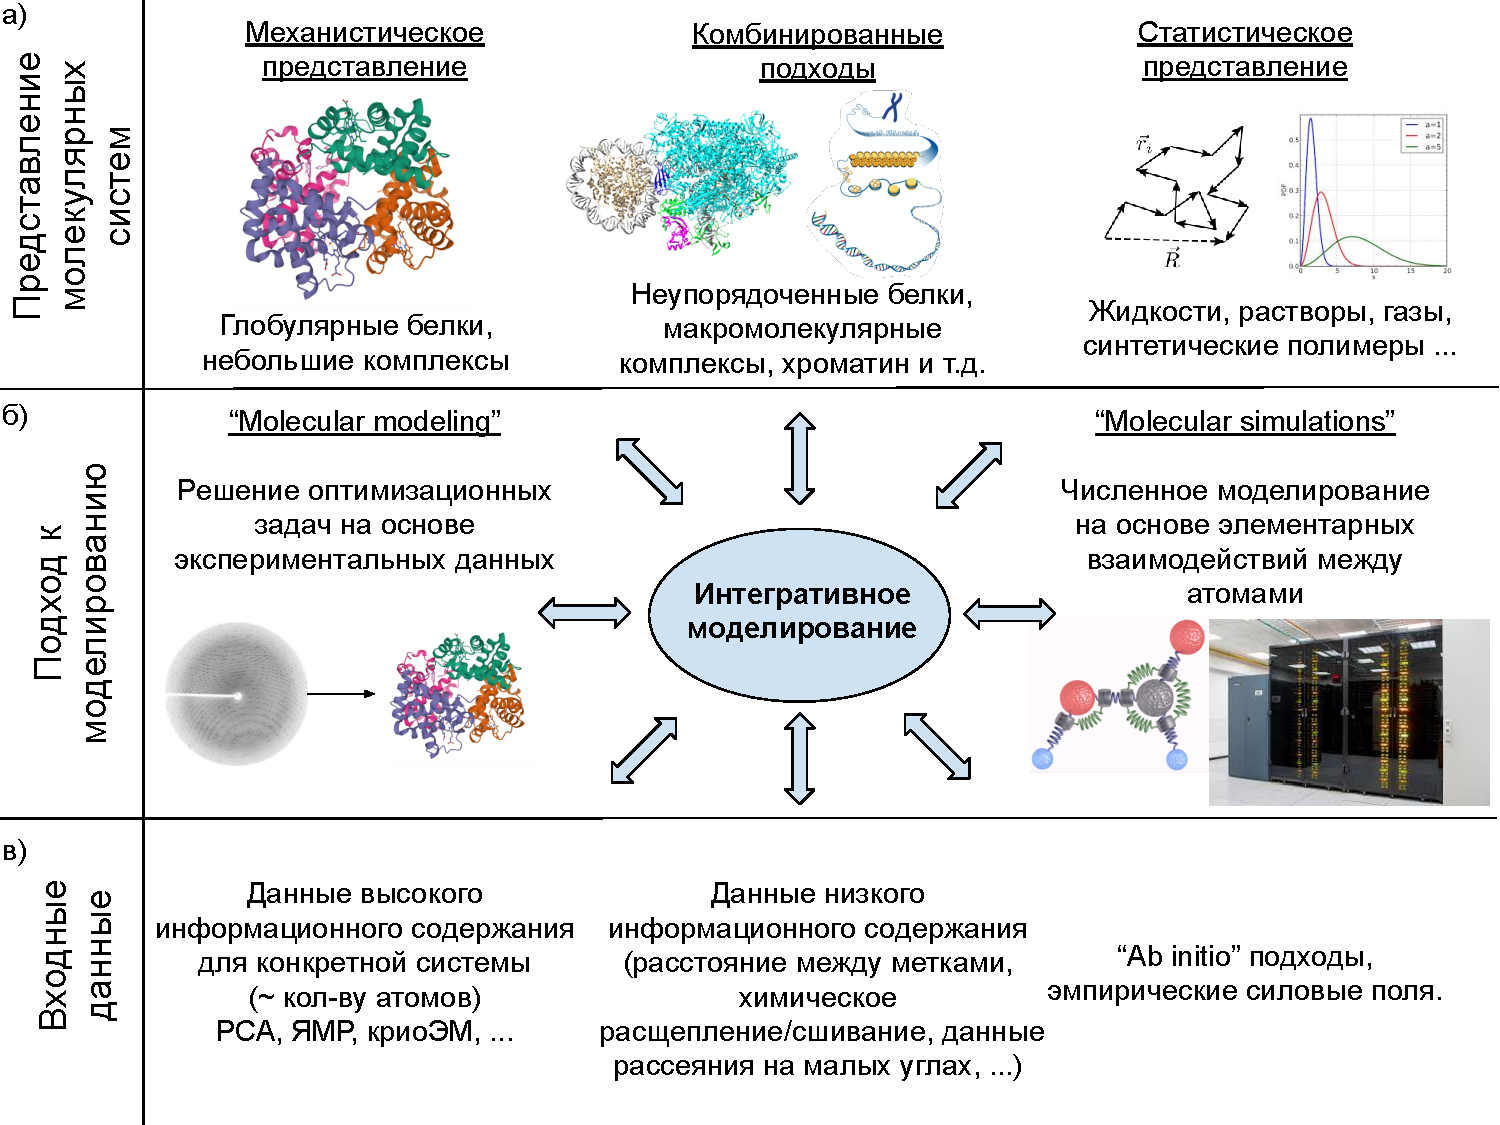
\includegraphics [width=\textwidth] {images/p1/concept_matrix.pdf}
%   \caption{Диаграмма, суммирующая различные подходы к описанию, моделированию и изучению структуры и динамики биомакромолекул.} 
%   \label{fig:p1:concept_matrix}
% \end{figure}


\begin{figure}[h!] 
 \center
 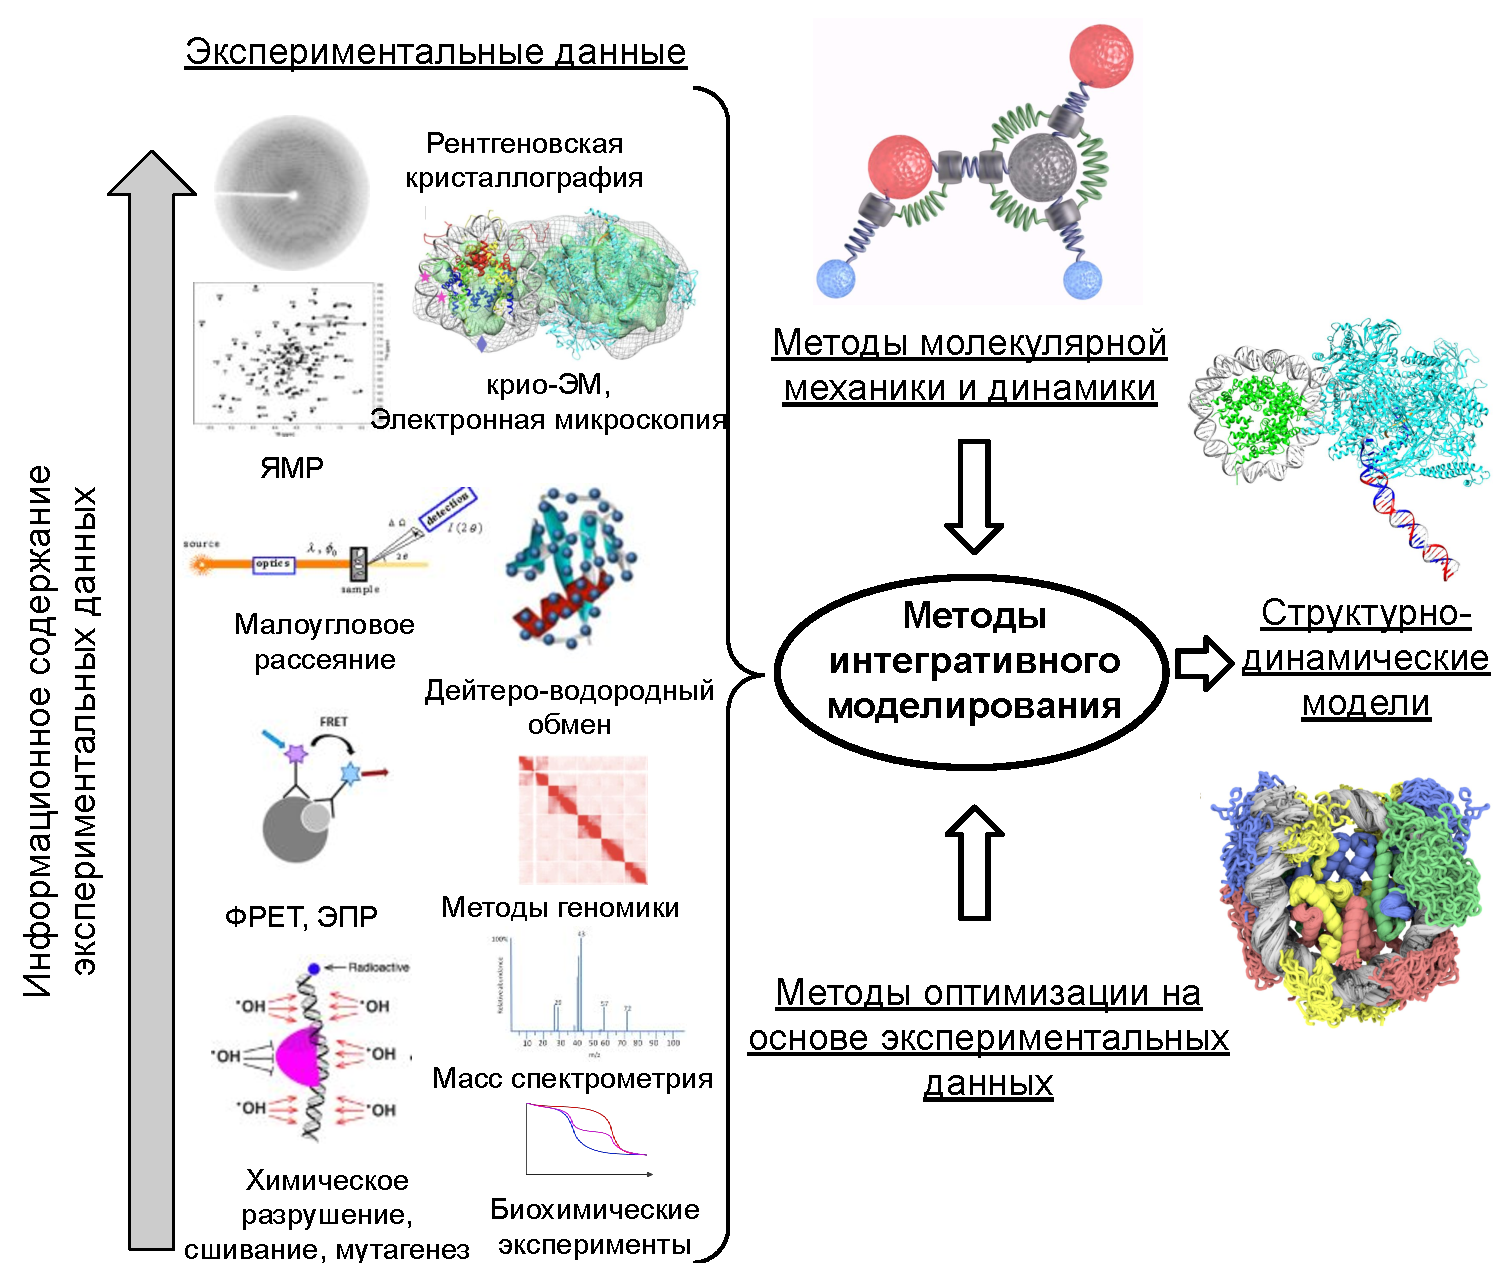
\includegraphics[width=\textwidth] {images/p1/int_mod.pdf}
 \caption{Идея методов интегративного моделирования.} 
 \label{fig:p1:int_mod}
\end{figure}





%\textit{Выводы главы 1} \\
%Исследование структуры многих биомакромолекулярных комплексов испытывает затруднения как при применении стандартных методов структурной биологии, так и при попытках атомистического моделирования на основе расчета атом-атомных взаимодействий. Методы интегративного моделирования, в ходе расчетов учитывающие как физические взаимодействия между атомами, так и экспериментальные данные различной природы, являются перспективным подходом для построения структурно-динамических моделей биомакромолекулярных комплексов. В главе предложены подходы по моделированию ДНК-белковых комплексов на основе моделей анизотропной гибкости ДНК с учетом разнородных экспериментальных данных.


В диссертационной работе метод молекулярной динамики является одним из важных компонентов разрабатываемых нами интегративных подходов. Понимание его возможностей и границ применимости необходимо для рационального выбора возможных стратегий моделирования. В связи с этим \underline{\textbf{вторая глава}} (\textit{Применение методов молекулярной динамики для изучения нуклеосом}) иллюстрирует современные возможности и ограничения метода суперкомпьютерной атомистической молекулярной динамики, направленного на получение и анализ структурно-динамических моделей биомакромолекулярных комплексов.

Нуклеосомы являются примером биомакромолекулярного комплекса существенных размеров (около 200 кДа) и играют важную роль в функционировании генома. Они состоят из примерно 200 пар оснований ДНК, организованных гистоновыми белками (Рис. \ref{fig:part2_1_f1}a). Центральные 145–147 пар оснований ДНК образуют коровую частицу нуклеосомы, плотно наматываясь на октамер гистонов в виде $\sim$1,7 витка левой суперспирали \cite{luger_crystal_1997,shaytan_nucleosome_2015,draizen_histonedb_2016}. Нуклеосомы претерпевают множество важных структурных и динамических перестроек во время всех ключевых процессов транскрипции, репликации, репарации ДНК и т.д. \cite{armeev_linking_2019}. Способность нуклеосом претерпевать определенные типы конформационных переходов играет важную роль при взаимодействии с белками, включая ремоделирующие комплексы, факторы транскрипции, шапероны \cite{valieva_large-scale_2016}, РНК-полимеразы \cite{gaykalova_structural_2015} и т.д.

  На рисунке \ref{fig:part2_1_f2}  проиллюстрированы предполагаемые динамические режимы нуклеосом и влияние на них различных факторов: 

\begin{figure} [h!]
    \centering
    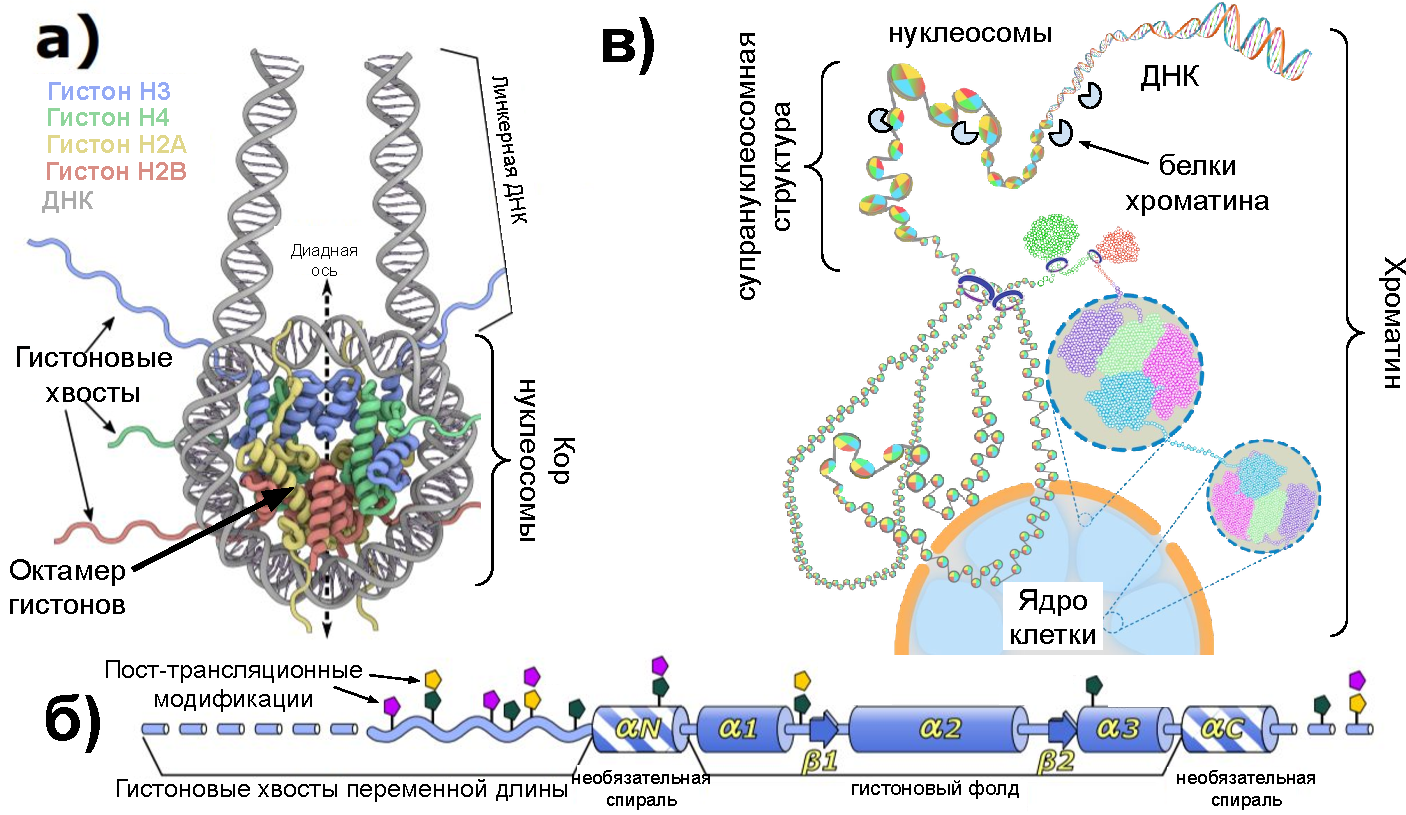
\includegraphics [width=\textwidth]{images/p2/cosb/part2_1_f1_synopsis.pdf}
    \caption[Структура и вариабельность нуклеосомы]{(a) Структура нуклеосомы. 
    (б) Схема типичной структуры гистонового белка и расположение пост-трансляционных модификаций.
    (в) Место нуклеосом в организации хроматина.}
    \label{fig:part2_1_f1}
\end{figure}

\noindent
последовательности ДНК и гистонов, пост-трансляционных модификаций аминокислот гистонов, взаимодействия с белками. Динамика нуклеосом может происходить спонтанно при данной температуре и носить функционально направленный характер за счет воздействия специальных АТФ-зависимых комплексов. Белковый состав и последовательность ДНК в нуклеосомах влияют на характер динамических процессов в нуклеосомах и таким образом модулируют различные функциональные процессы в геноме. Так показано существование тонких режимов конформационной динамики нуклеосом \cite{armeev_linking_2019}. Например, кручение ДНК внутри нуклеосомы обеспечивает путь для АТФ-зависимого ремоделирования нуклеосом \cite{bowman_remodeling_2019}. Речь идет о существовании особых режимов динамики нуклеосом, в которых важны атомистические детали структурных изменений. Метод молекулярной динамики является мощным инструментом, который может раскрыть природу этих динамических режимов.





\begin{figure} [h!]
    \centering
    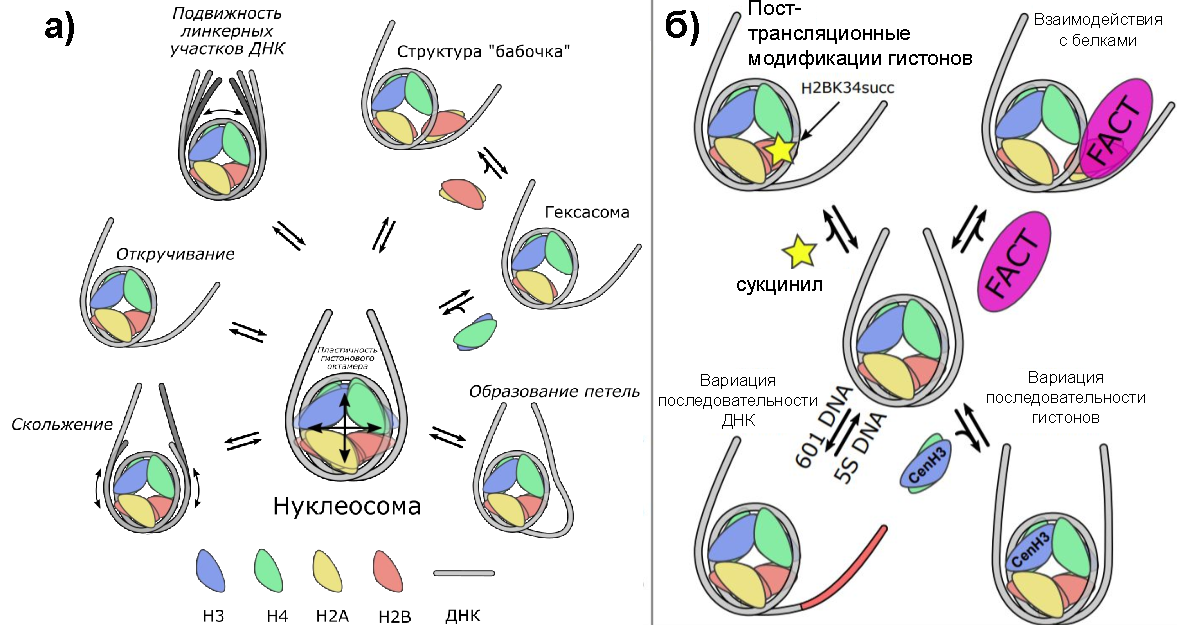
\includegraphics [width=\textwidth]{images/p2/cosb/part2_1_f2_synopsis.pdf}
    \caption[Моды динамики нуклеосом]{(а) Иллюстрация некоторых мод динамики нуклеосом. (б) Примеры факторов, влияющих на структурную динамику нуклеосом.}
    \label{fig:part2_1_f2}
\end{figure}

Для этого нами были разработаны подходы и алгоритмы моделирования нуклеосом методами молекулярной динамки в полноатомном приближении в микросекундном временном диапазоне с использованием суперкомпьютерных технологий. Разработаны алгоритмы подготовки систем для моделирования и анализа динамического поведения нуклеосом в явном растворителе. В частности, разработаны алгоритмы задания нуклеосомной системы координат на основе определения оси суперспирали ДНК и оси псевдосимметрии нуклеосомы. В результате стало возможным определение различных геометрических параметров молекулярной системы таких, как геометрия ДНК, углы вращения ДНК, расположение остова полипептидных цепей.
  

В \textit{разделе 2.2} приводятся результаты равновесного микросекундного моделирования молекулярной динамики нуклеосом, включающих линкерные сегменты ДНК и полноразмерные гистоны (рисунок \ref{fig:part2_1_f1}), в явном растворителе в атомистическом приближении.
%Впервые мы смогли идентифицировать и охарактеризовать перестройки в нуклеосомах на микросекундном масштабе времени, изучить связь между конформацией гистоновых хвостов и геометрией ДНК. 
Было выявлено, что линкерные участки ДНК изменяют свое взаимное расположение из-за электростатического отталкивания, что влияет на углы входа-выхода ДНК из нуклеосом и следовательно на структуру супрануклеосомной организации хроматина. Мы показали, что определенные конформации гистонового хвоста способствуют выпячиванию ДНК вблизи участков ее входа/выхода в/из нуклеосомы, что приводит к образованию дефектов кручения внутри ДНК. Показано, что если в начальной структуре гистоновые хвосты экспонированы в растворитель, то в ходе динамики их конденсация на ДНК происходит в течение нескльких десятков наносекунд. Далее начинается диффузия хвостов вдоль поверхности ДНК. При этом хвосты могут принимать конформационно ограниченные позиции из-за вставки  лизинов и аргининов в малые бороздки ДНК. Ряд аминокислот в гистоновых хвостах, являются сайтами важных эпигенетических пост-трансляционных модификаций (см. рисунок \ref{fig:part2_1_f1}б) и сайтами связывания белков хроматина (например, H3K9, H3K27, H4K16). На рисунке \ref{fig:p2_2_f1}в видно, что многие из этих сайтов находятся в тесном контакте с ДНК, что ограничивает их доступность для пост-трансляционной модификации и взаимодействий с белками хроматина. В то же время, такие взаимодействия способствуют возникновению кооперативных эффектов при связывании нескольких белков с соседними сайтами на гистоновых хвостах. Полученные результаты находятся в согласии  с рядом экспериментов по химическому сшиванию гистонов с ДНК, анализу влияния хвостов на взаимодействия белков хроматина с нуклеосомами.  Рисунок \ref{fig:p2_2_f1} суммирует наблюдавшуюся конформационную подвижность нуклеосом.


\begin{figure} [H]
    \centering
    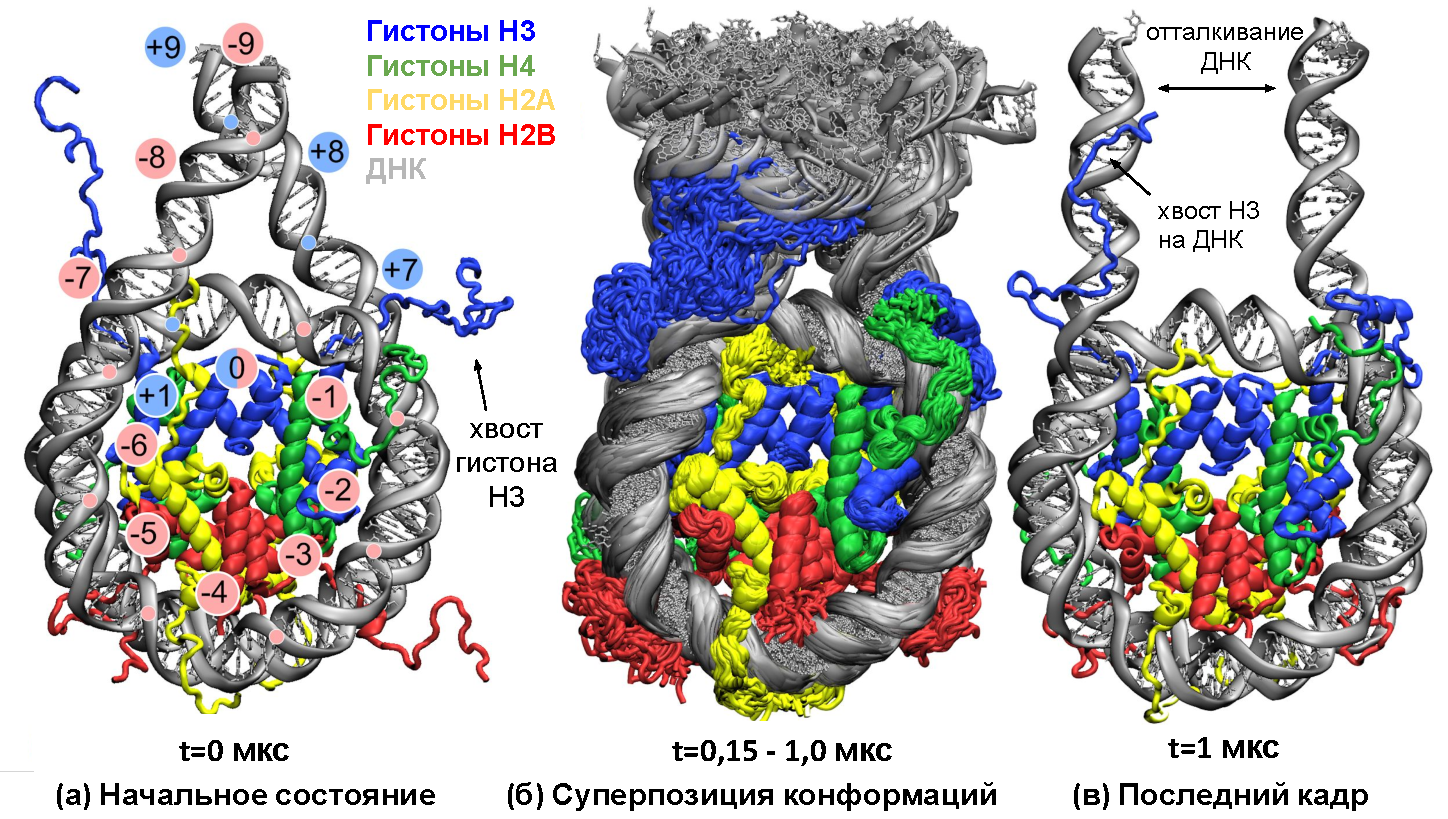
\includegraphics[width=\textwidth]{images/p2/jmb/part2_2_f1.pdf}
    \caption{Изменение конформации нуклеосомы в течение 1 мкс в ходе расчетов методом молекулярной динамки. На исходном состоянии (а) цифрами отмечены супер-спиральные положения ДНК, где большая бороздка ДНК обращена в сторону октамера гистонов. В ходе динамики (б-в) наблюдается динамическая подвижность линкерных сегментов ДНК, сопровождающаяся их отталкиванием, а также конденсация хвостов на линкерную и нуклеосомальную ДНК.}
    \label{fig:p2_2_f1}
\end{figure}

 

\begin{figure} [H]
    \centering
    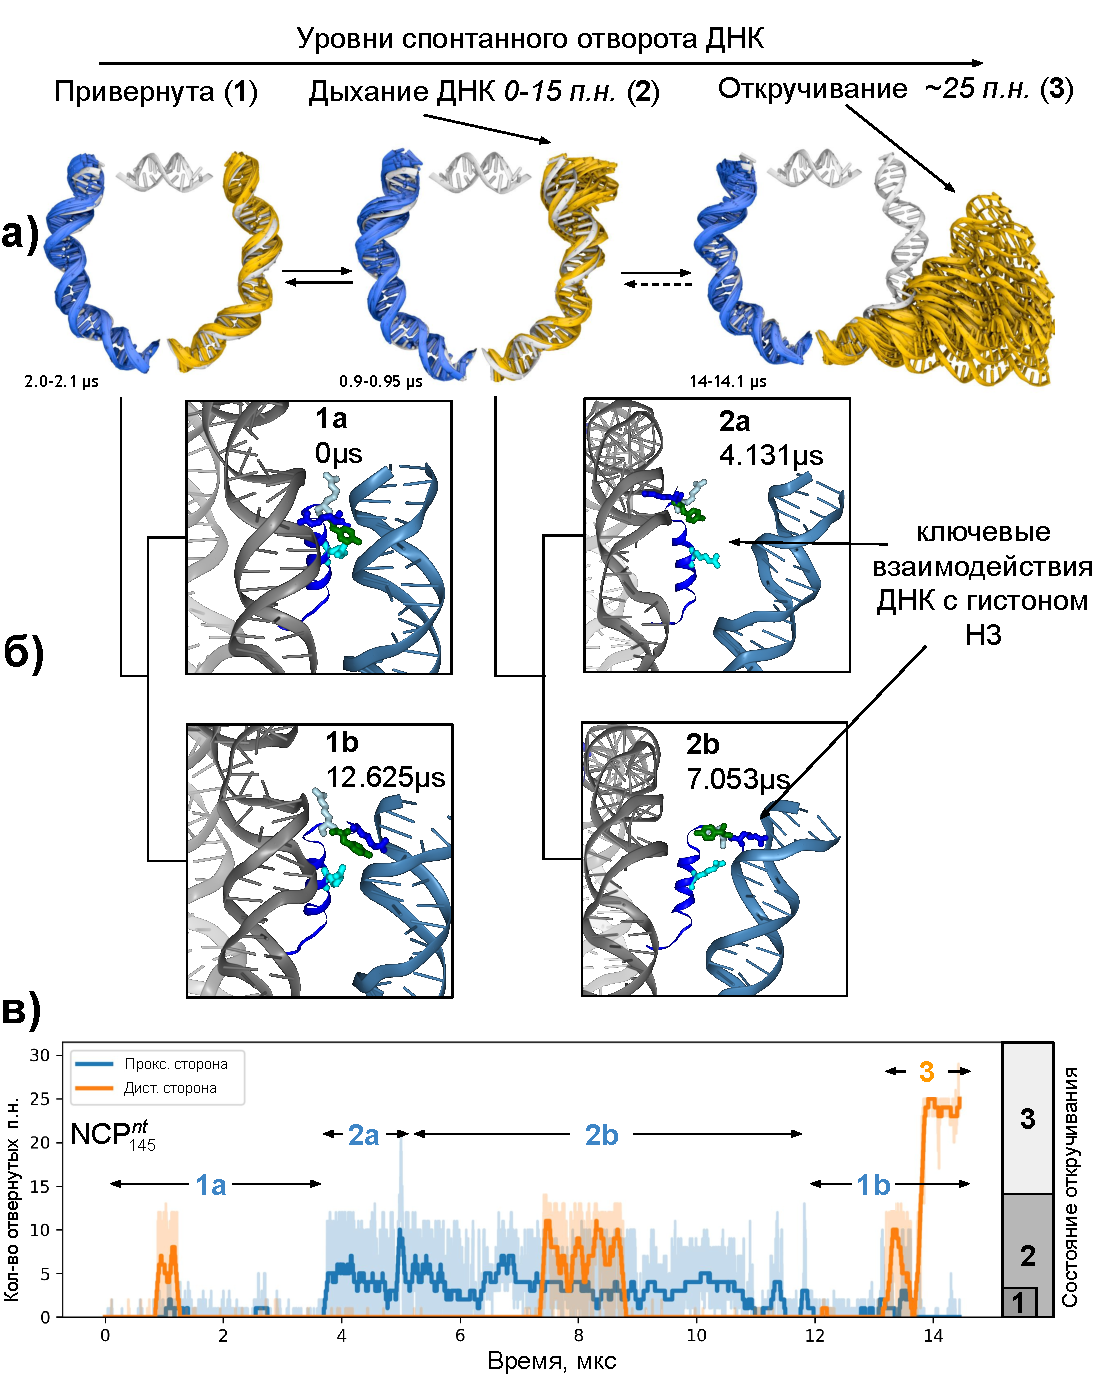
\includegraphics[width=\textwidth]{images/p2/10ms/fig2_new.pdf}
    \caption[Динамика отворота ДНК в нуклеосоме с укороченными гистоновыми хвостами]{Динамика отворота ДНК в нуклеосоме с укороченными гистоновыми хвостами. (а) Наблюдаемые динамические состояния \textbf{1-3}, между которыми система переходит в ходе динамики. (б) Для состояний \textbf{1} и \textbf{2} наблюдаются подсостояния, связанные с реориентацией белкового сегмента в районе H3 $\alpha$N спирали (область H3-``застежки''). (в) Количество пар нуклеотидов отвернутых от октамера гистонов как функция времени моделирования. Критерий отворота ДНК  --  смещение центра пары оснований более, чем на 7 \AA{} от положений оснований в исходной структуре. }
    \label{fig:p2_3:f2}
\end{figure}



Результаты  моделирования коровых частиц нуклеосом методом молекулярной динамики приведены в \textit{разделе 2.3}. Разработанные нами оригинальные алгоритмы моделирования позволили получить динамические траектории нуклеосомного кора с полноразмерными гистоновыми хвостами при физиологической температуре и ионной силе на временах более 10 микросекунд. 
 С помощью специально разработанных алгоритмов анализа траекторий (проекция координат в системе отсчета нуклеосом, расчет относительного скручивания ДНК, анализ стабильных контактов и т. д.) мы выявили новые режимы динамики и пластичности нуклеосом. Мы показали возможность реконфигурации и разворачивания концов ДНК в нуклеосомах, опосредованных гистоновыми хвостами H3 и H2A. Выявленные режимы отворачивания ДНК представлены на рисунке \ref{fig:p2_3:f2}а. В ходе моделирования были выявлены ключевые взаимодействия ДНК-белок с гистонами, которые являются барьерами для откручивания ДНК от октамера гистонов (рисунок \ref{fig:p2_3:f2}б). В ходе моделирования также была показана возможность локального спонтанного изменения степени закрученности ДНК (образование/релаксация так называемых дефектов кручения) и сдвиг ориентационного положения для части коровой ДНК. Данные наблюдения указывают на возможность транслокации ДНК вдоль нуклеосомы путем ``червячного'' передвижения дефектов кручения вдоль ДНК (inchworm meсhanism). При этом ДНК подобно винту прокручивается вдоль поверхности октамера гистонов. В ходе моделирования было показано наличие динамической пластичности ядра гистонов, способствующей подвижности ДНК. В результате сравнительного моделирования коровых частиц нуклеосом с хвостами и без хвостов гистонов было выявлено, что гистоновые хвосты замедляют как время отворота, так и время приворота ДНК, а также при отвороте ДНК удерживают ее вблизи исходной траектории. Показано, что область гистона H3, находящаяся между двумя супервитками ДНК (см. среднюю часть Рис. \ref{fig:p2_3:f2}), играет важную роль в стабилизации концов ДНК, а также влияет на стабильность ДНК вблизи диады нуклеосомы.

Результаты, приведенные в данной главе, основаны на следующих ключевых статьях  
 \cite{shaytan_coupling_2016,hada_histone_2019,bass_effect_2019,armeev_linking_2019,gribkova_investigation_2017,el_kennani_ms_histonedb_2017,shaytan_trajectories_2016,shaytan_coupling_2016,draizen_histonedb_2016,armeev_nucleosome_2016,shaytan_nucleosome_2015,armeev_conformational_2015,armeev_molecular_2015}.






\textit{Выводы главы 2} \newline
%В главе 2 на примере моделирования нуклеосом продемонстрированы возможности современных технологий суперкомпьютерного моделирования динамики биомакромолекулярных комплексов в атомистическом приближении на микросекундных временных масштабах.  Показано, что для комплексов ДНК-белок такого размера (около 200 кДа) современные методы равновесной МД позволяют исследовать крупномасштабную динамику, связанную с отворотом/приворотом ДНК, диффузией неупорядоченных белковых хвостов воль ДНК.  На основании моделирования могут быть сформулированы также следующие научные выводы и гипотезы важные с точки зрения понимания функционарования нуклеосом:

 
\begin{itemize}
    \item Электростатическое отталкивание двух сегментов линкерной ДНК является одним из факторов, которые влияют на конформацию ДНК и углы входа-выхода ДНК из ядра нуклеосомы.
    \item В процессе спонтанного ступенчатого откручивания/прикручивания ДНК в нуклеосоме последовательно теряются стабильные взаимодействия ДНК с гистонами. Конформация ДНК подвержена значительным флуктуациям в наносекундном диапазоне. В переходе нуклеосом из кристаллоподобного состояния в состояние с отвернутой ДНК ключевую роль играют взаимодействия остатков гистона H3 между двумя супервитками ДНК.
   % \item Показано, что спонтанное откручивание ДНК от нуклеосомы приводит к разрыхлению структуры хроматиновых фибрилл.
    \item Формирование дефектов кручения ДНК в нуклеосоме и конформационные перестройки внутри глобулярных частей гистонового октамера, происходящие на микросекундных временах, указывают на возможность скольжения нуклеосом вдоль ДНК по винтовому механизму и транслокацию ДНК вдоль октамера.
  %  \item Гистоновые хвосты в нуклеосоме активно взаимодействуют с коровой и линкерной ДНК, влияют на кооперативность взаимодействия белков хроматина с гистоновыми хвостами.
  %  \item Конформационные перестройки внутри глобулярных частей гистонового октамера, происходящие на микросекундных временах, влияют на подвижность ДНК и, вероятно, эффективность транслокации ДНК вдоль октамера.
   % \item Показано наличие аллостерических эффектов между откручиванием концов ДНК в нуклеосоме и стабильности центральной части ДНК, важные с точки зрения передвижения нуклеосом вдоль ДНК.  
\end{itemize}


%Ниже бывшая третья глава.
%\underline{\textbf{Третья глава}} (\textit{Расчет свободной энергии гидратации и адсорбции аминокислот}) иллюстрирует применение подходов молекулярного моделирования, позволяющих вычислять экспериментально измеримые термодинамические характеристики на основе молекулярно-динамических атомистических моделей.
%В главе речь идет об изучении гидратации боковых цепей аминокислот вблизи поверхности воды путём построения профилей свободной энергии на основании классических атомистических моделей молекул. Работа также имеет методологическое значение, поскольку в ней впервые предприняты попытки высокоточной численной оценки термодинамических параметров гидратации и адсорбции.

%Для расчёта профиля свободной энергии соединений на границе раздела фаз вода/пар была сконструирована модель границы раздела - прямоугольный слой воды толщиной 4 нм. Для расчёта профиля свободной энергии использовался метод удерживающей силы. На каждом шаге измерялась удерживающая сила, которую необходимо было прикладывать, чтобы удерживать исследуемое соединение на определенном расстоянии от границы раздела фаз. Интегрированием профиля средней силы вычислялся профиль свободной энергии. Измерение энергии адсорбции проводилось двумя предложенными способами: используя подход Гиббса и путём измерения значения профиля энергии в минимуме. В подходе Гиббса сначала рассчитывался относительный профиль концентрации, предполагая концентрацию в газовой фазе равной 1 нм$^{-3}$. Затем рассчитывался избыток энергии Гиббса по формуле \ref{excess}, а энергия адсорбции оценивалась по формуле \ref{ads_fe_eq}, предполагая толщину границы раздела равной 1 нм, поскольку это обычно была величина, на которой варьировался профиль свободной энергии.
%Оба набора полученных энергий  находятся в отличной корреляции между собой (R=0.9996), хотя заметны некоторые отклонения для веществ с низкой поверхностной активностью, для последних, очевидно, выбор метода имеет значение. Хотя значение энергии в минимуме оказалось хорошей оценкой энергии адсорбции, предположительно метод Гиббса является более универсальным и термодинамически корректным. Примеры полученных профилей свободной энергии приведены на рисунке \ref{4pmf}.


%\begin{equation}
%\Gamma^i=\int_{-\infty}^{z_0}(c^i(z)-c^i_1)dz+\int_{z_0}^{\infty}(c^i(z)-c^i_2)dz
%\label{excess}
%\end{equation}

%\begin{equation}
%G_{ads}=-kT\ln{\frac{\Gamma^S}{c^S\tau}}
%\label{ads_fe_eq}
%\end{equation}

%\begin{figure}[h!]
%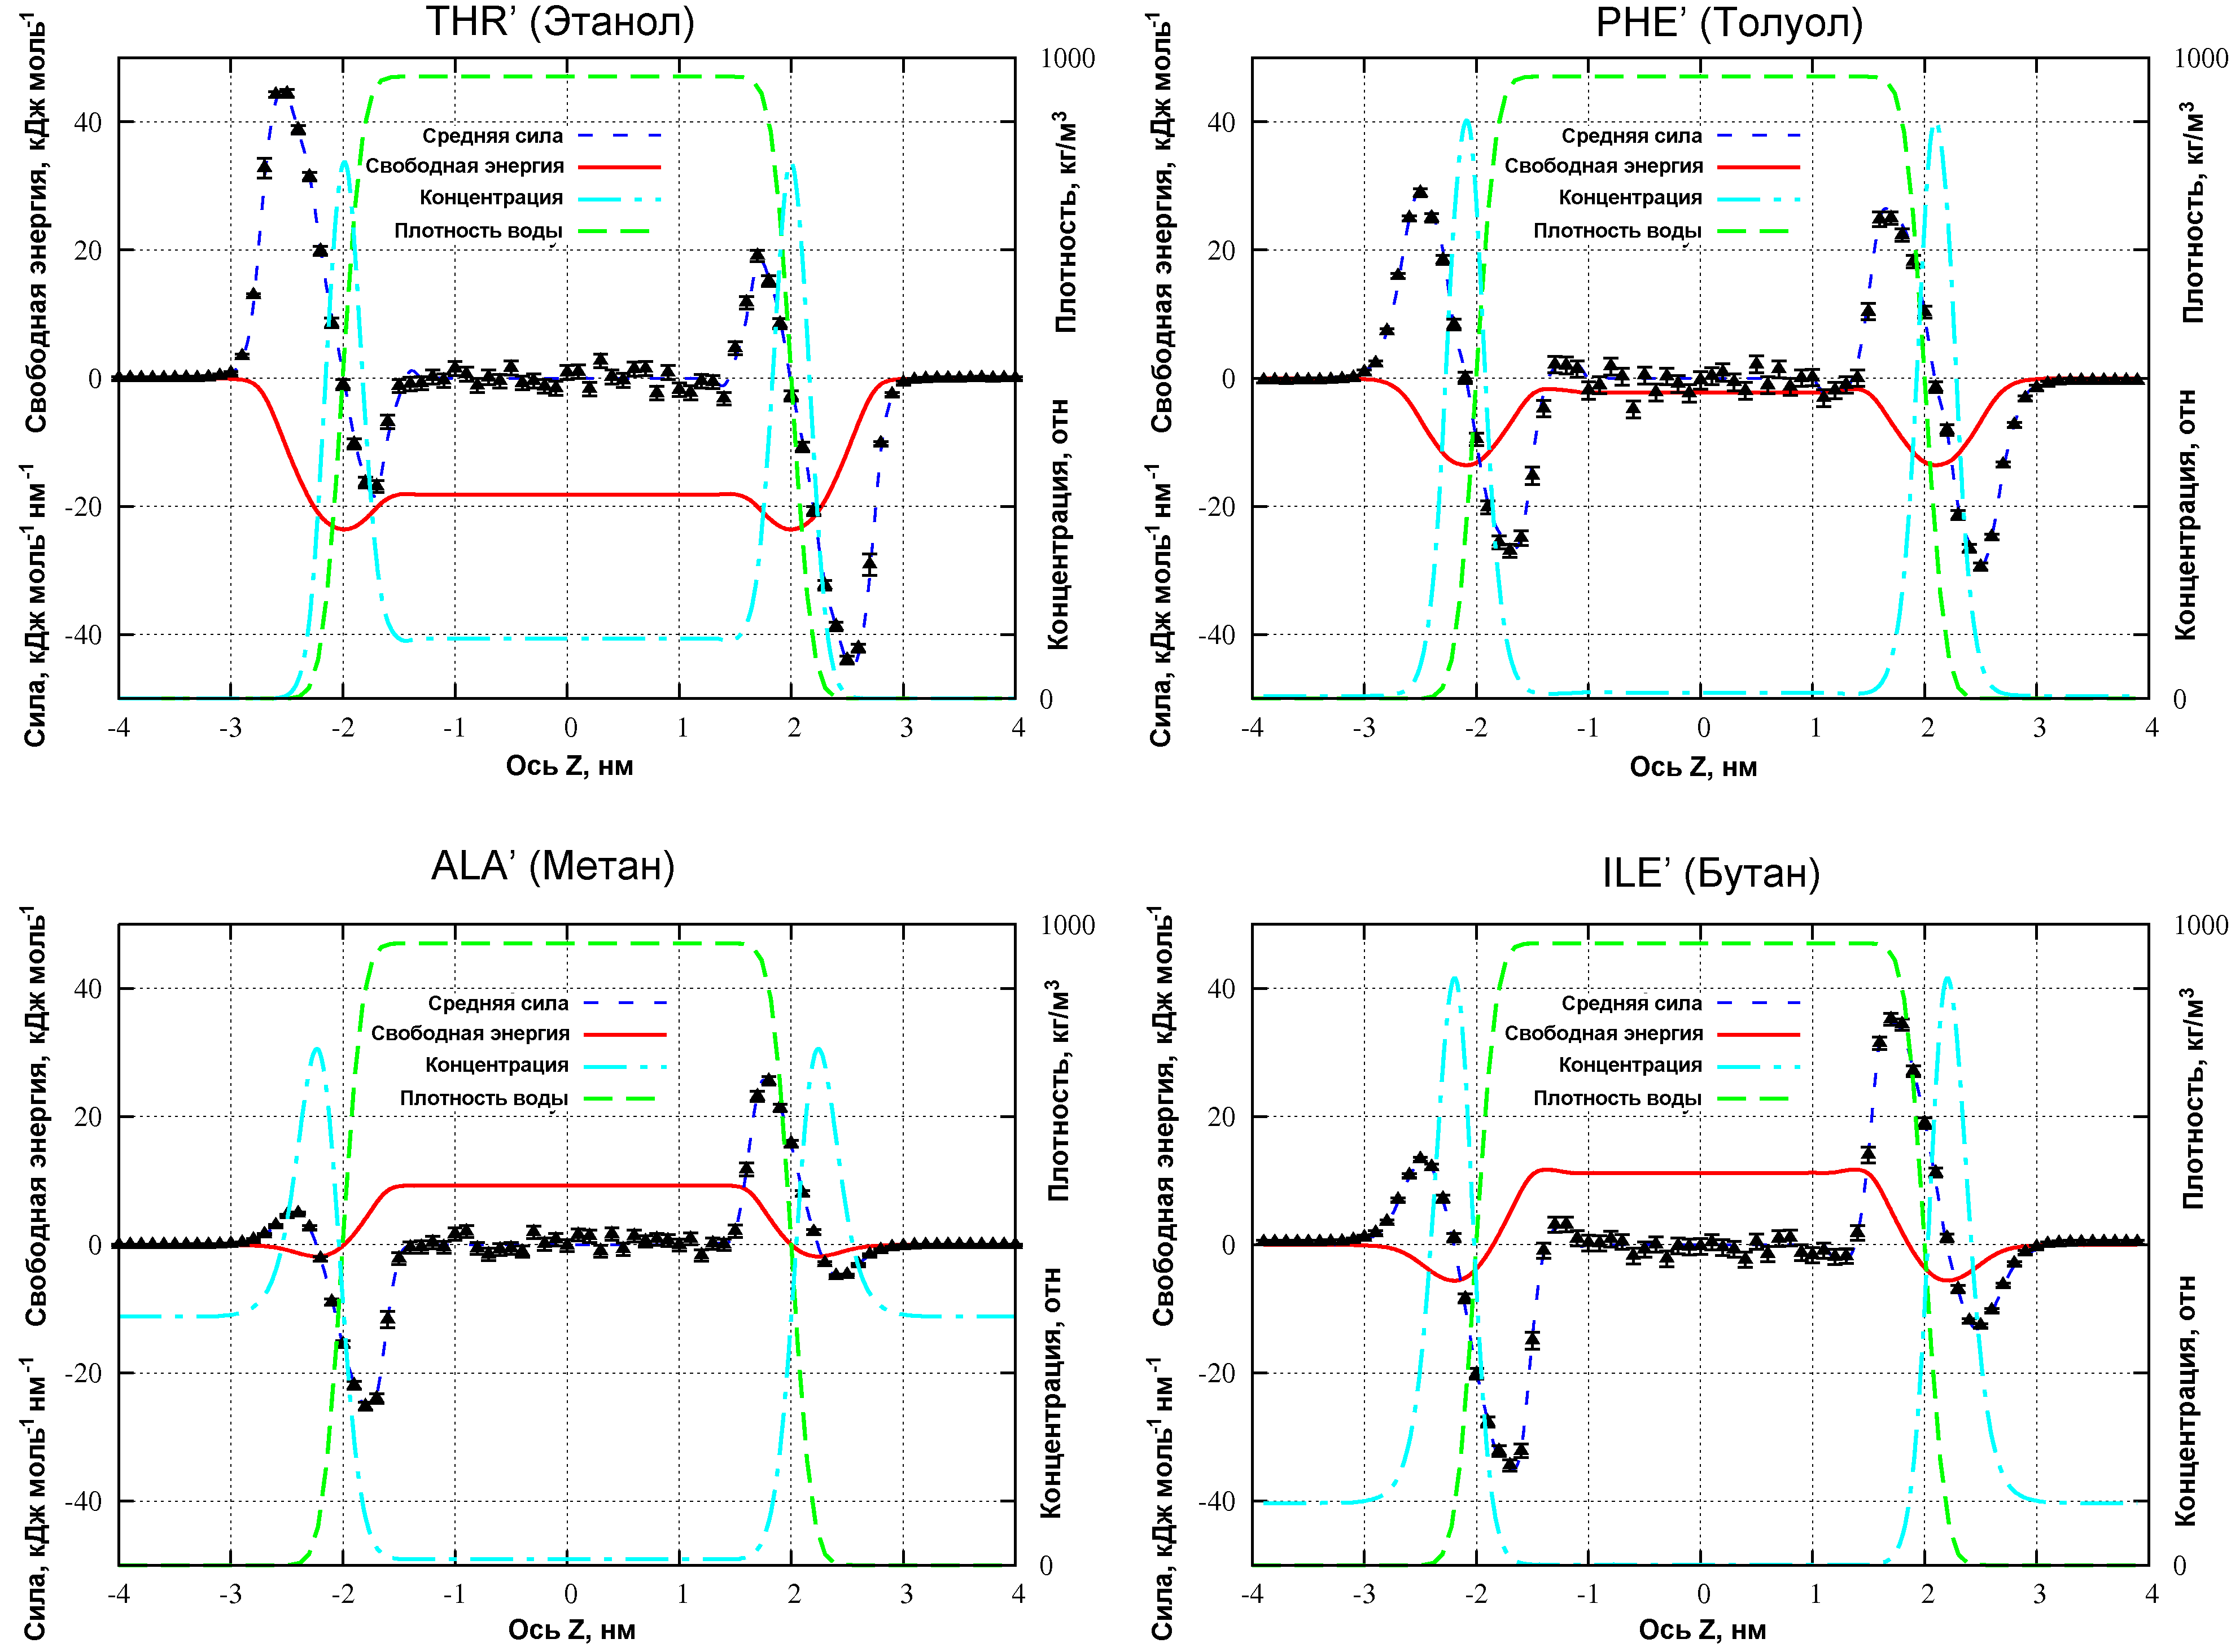
\includegraphics[width=\textwidth]{images/p3/4pmf}
%\caption{\label{4pmf} Профили свободной энергии для нескольких изученных молекул. Пунктирные линии и точки с отмеченными погрешностями - профиль средней силы и его сплайн аппроксимация (погрешности отмечены как $\pm$ одно стандартное отклонение). Сплошная линия - профиль свободной энергии, пунктирно-точечная линия - относительный профиль концентрации, рассчитанный по профилю свободной энергии. Для сравнения пунктирной линией отмечен профиль плотности водного слоя.}
%\end{figure}

%Материалы данной главы основаны на следующих статьях \cite{shaytan_free_2010,shaytan_solvent_2009}. 

%\textit{Выводы главы 3} \newline
%По результатам работы, изложенной в главе 3, можно сделать следующие выводы, обладающие научной новизной:
%\begin{itemize}
%\item Профили средней силы для боковых цепей аминокислот на границе вода-воздух приблизительно одинаковы по форме: имеют область притяжения перед поверхностью Гиббса со стороны воздуха, и достаточно узкую (0.6-0.7 нм) область выталкивания за поверхностью Гиббса.
%\item Вывод об одинаковой форме профилей средней силы на границе вода/воздух, по-видимому, можно обобщить на весть класс небольших незаряженных молекул.
%\item В использованной модели, видимые поверхностные эффекты сольватации для боковых цепей аминокислот исчезают, когда центр масс молекулы погружён на 0.6-0.7 нм в воду по отношению к поверхности Гиббса, что может считаться эффективной глубиной границы раздела для маленьких молекул.
%\item Профили свободной энергии для всех молекул обладают минимумом в районе границы раздела, который является результатом баланса между силами притяжения, доминирующими со стороны воздуха, и силами отталкивания, доминирующими со стороны воды, и имеющими энтропийную природу.
%\item Глубина минимума свободной энергии находится в хорошей корреляции с энергией адсорбции, рассчитанной по методу Гиббса.
%\item С высокой точностью вычислены энергии гидратации и адсорбции для 13 незаряженных веществ-аналогов боковых цепей аминокислот.
%\item Показано, что энергия адсорбции из газовой фазы для выбранного набора боковых цепей аминокислот находиться в хорошей корреляции с энергией гидратации.
%\item Энергия адсорбции относительно фазы максимального сродства не коррелирует с энергией гидратации и может использоваться как независимая термодинамическая характеристика молекул вещества.
%\item Полученные данные для нескольких молекул согласуются с экспериментальными данными и могут применяться для совершенствования силовых полей, однако достоверных систематических данных по оценки энергии адсорбции для всей группы веществ на границе вода-воздух пока в литературе не обнаружено.
%\end{itemize}


Процессы динамики нуклеосом, изученные нами методом МД, ограничены по времени в силу текущих вычислительных возможностей. Крупномасштабные процессы, например, скольжения нуклеосом вдоль ДНК, сборка и разборка нуклеосом, полная диссоциации/реассоциации ДНК пока находятся за пределами моделируемых временных интервалов. Примером задачи не решаемой методами МД является выбор нуклеосомой наиболее энергетически выгодного оптимального положения на большом участке ДНК. Для решения такой задачи могут применяться интегративные подходы, изложенные в \underline{\textbf{третьей главе}} (\textit{Интегративное моделирование с применением данных экспериментов по футпринтингу ДНК}). В главе развиты подходы по моделированию ДНК-белковых комплексов, основанные на использовании экспериментальных данных по расщеплению ДНК (футпринтингу) гидроксильными радикалами. Гидроксильные радикалы обладают высокой реакционной способностью, небольшим размером, не являются заряженными. При взаимодействии с ДНК они атакуют атомы водорода дезоксирибозы, что приводит к расщеплению ДНК с потерей атакованного нуклеотида. При наличии белка на ДНК, белок стерически экранирует ДНК от расщепления. Это свойство можно использовать для анализа структуры ДНК-белковых комплексов. Общая схема данного подхода представлена на рисунке \ref{fig:p5_1_f1}.

 Комплексы ДНК-белок создаются с использованием радиоактивно меченной ДНК и подвергаются расщеплению гидроксильными радикалами преимущественно на участках, не защищенных белком. Репертуар расщепленных фрагментов ДНК анализируется с помощью денатурирующего гель-электрофореза. По интенсивности полос в геле можно судить о вероятности расщепления ДНК в том или ином месте последовательности. Атомистические структурные модели могут использоваться для прогнозирования профилей футпринтинга, поскольку частота расщепления зависит от доступности атомов водорода дезоксирибозы. Сравнение предсказанных и экспериментальных результатов может быть использовано для уточнения или создания структурных моделей. Несмотря на кажущуюся простоту данной концепции, ее комплексное решение представляет собой нетривиальную задачу, требует подбора алгоритмов анализа данных, их оптимизацию и программную реализацию. Нами такие алгоритмы были реализованы в виде программного комплекса HYDROID \cite{shaytan_structural_2018} (\url{https://github.com/ncbi/HYDROID}). Ключевой задачей решаемой пакетом HYDROID является количественная оценка частоты расщепления ДНК в каждом положении на основе анализа изображений гель электрофореза, а также теоретическая количественная оценка этого параметра на основе атомистических структурных моделей.

\begin{figure} [H]
    \centering
    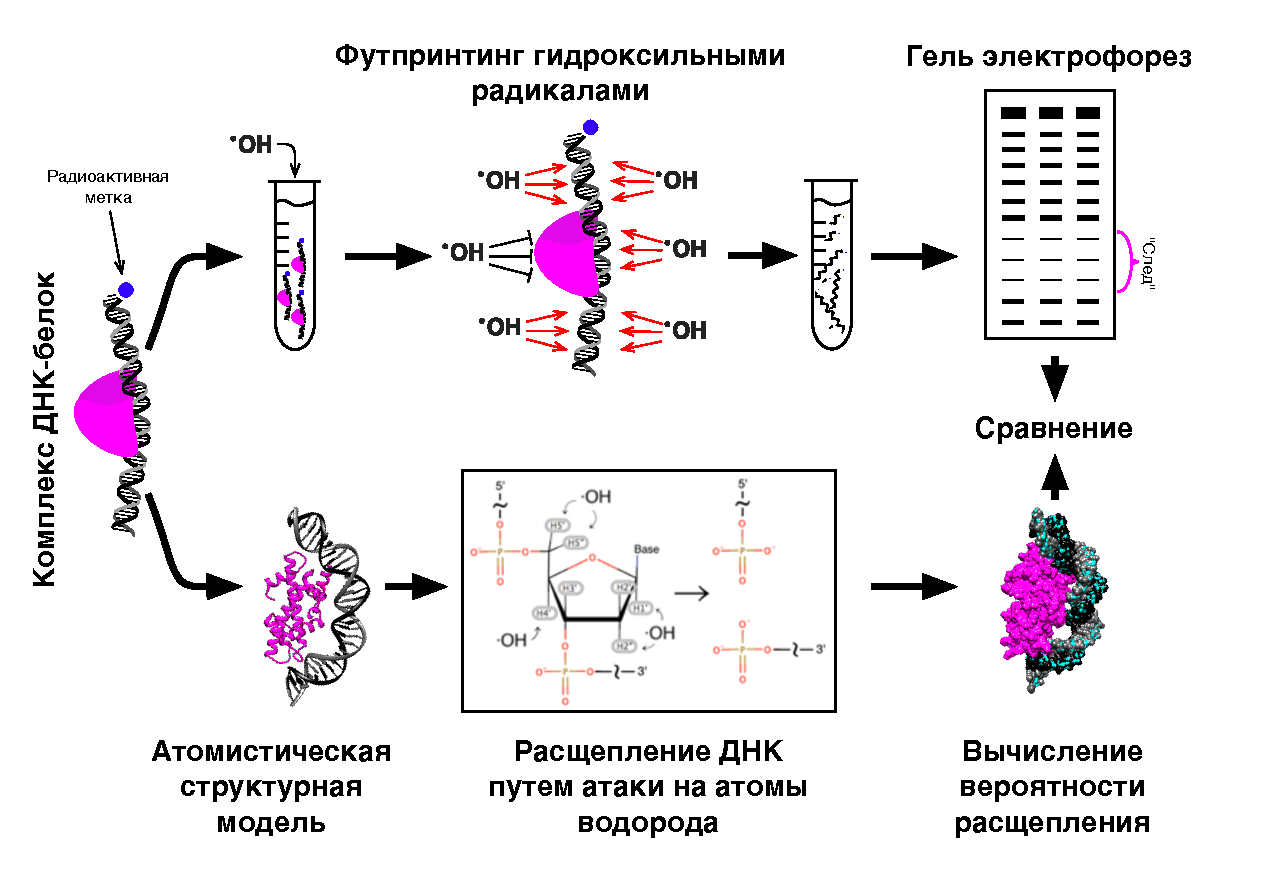
\includegraphics[width=\textwidth]{images/p5/part5_1_np/p5_1_f1.pdf}
    \caption[Футпринтинг комплексов ДНК-белок гидроксильными радикалами и структурная интерпретация экспериментальных данных.]{Футпринтинг комплексов ДНК-белок гидроксильными радикалами и структурная интерпретация экспериментальных данных. }
    \label{fig:p5_1_f1}
\end{figure}
 
Процесс деконволюции изображения дорожек геля в частоты расщепления ДНК представлен на рисунке \ref{fig:p5:p5_2_f5} и предполагает аппроксимацию профиля дорожки в виде суммы кривых Гаусса или Лоренца, описывающих вклад каждой полосы на геле. Математическая процедура данной аппроксимации была реализована в виде многопараметрической оптимизации аналитической функции (являющейся суммой вкладов отдельных пиков) по методу наименьших квадратов на основе алгоритма Левенберга — Марквардта. Данная процедура не всегда приводит к физически обоснованному решению и может быть неустойчива. Поэтому были разработаны дополнительные методы регуляризации решений, накладывающие ограничения на положения и ширину отдельных Гауссианов/Лоренцианов.



Для предсказания вероятности расщепления ДНК по атомистическим структурам были разработаны методы расчета поверхности атомов водорода дезоксирибозы доступной растворителю (H-SASA). Данный параметр чувствителен к небольшим вариациям в геометрии ДНК, параметрам выбираемым для длин атом-атомных связей и размерам атомов. Были проведены наборы расчетов методом молекулярной динамики для выяснения влияния динамических эффектов на профили H-SASA и вычисления наиболее точных профилей H-SASA. В результате были предложены процедуры (в том числе способы добавления атомов водорода к тяжелоатомным структурам) и наборы параметров для оценки профилей H-SASA по кристаллическим структурам.

\begin{figure}[H]
    \centering
    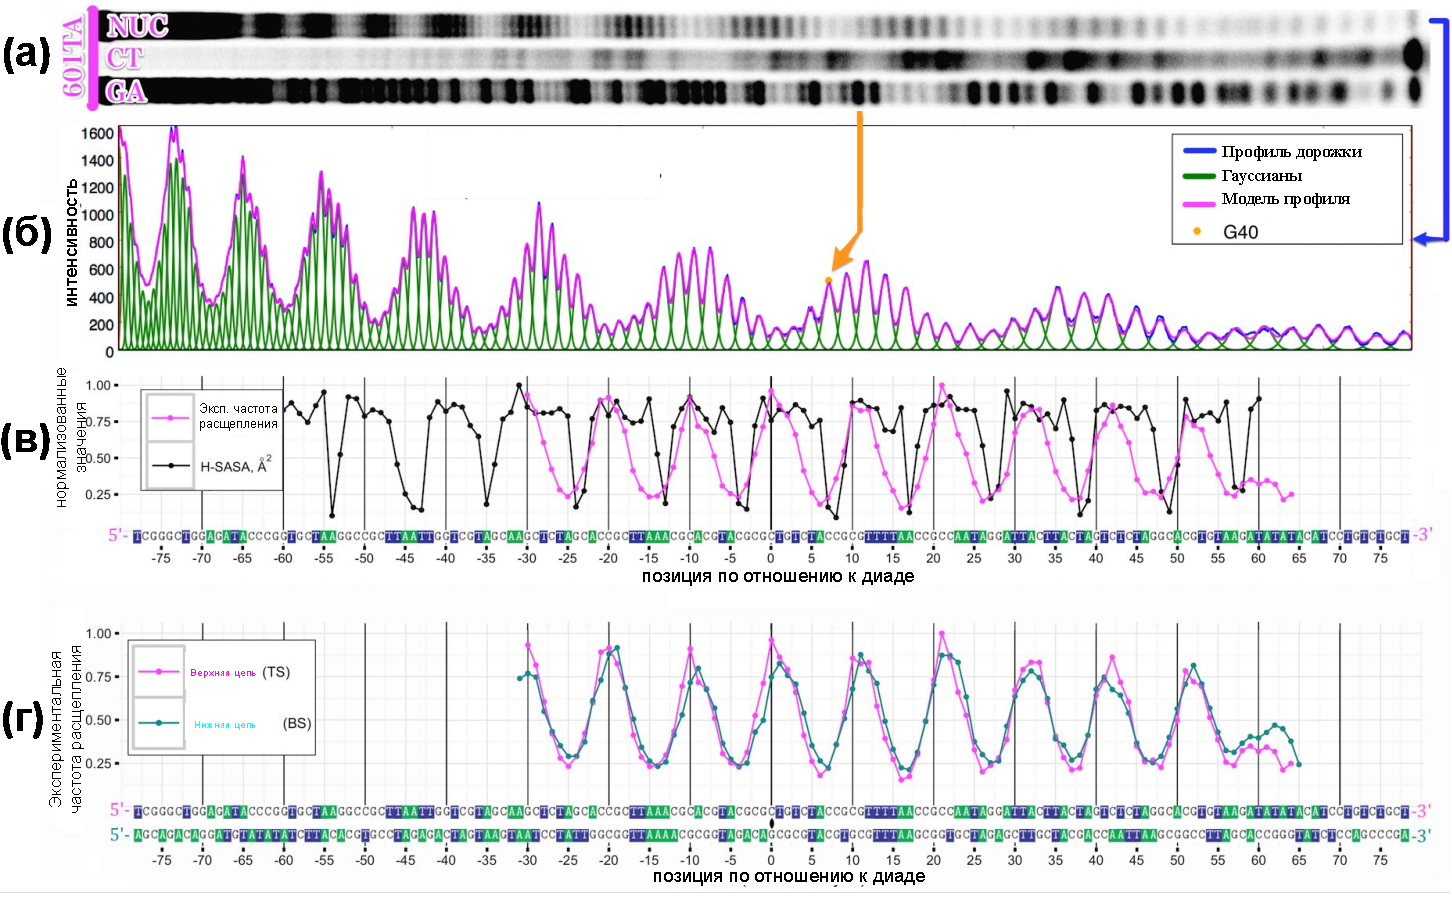
\includegraphics[width=\textwidth]{images/p5/part5_2_nar/p5_2_f5.pdf}
    \caption[Количественная оценка экспериментов по гидроксильному футпринтингу и сравнение с теоретическими профилями, полученными на основе атомной структуры известной нуклеосомы (601TA-NUC)]{Количественная оценка экспериментов по гидроксильному футпринтингу и сравнение с теоретическими профилями, полученными на основе атомной структуры известной нуклеосомы (601TA-NUC). (A) Изображение полиакриламидного геля с продуктами реакции для верхней цепи ДНК. (Б) Профиль интенсивности дорожек геля и его деконволюция в индивидуальные интенсивности полос путем подбора функций Гаусса. (В) суперпозиция количественных экспериментальных частот расщепления ДНК и профилей H-SASA, рассчитанных на основе атомистической структуры. (Г) Суперпозиция экспериментальных частот расщепления ДНК для верхней и нижней цепей ДНК.}
    \label{fig:p5:p5_2_f5}
\end{figure}


На основании разработанных подходов были изучены данные по расщеплению ДНК в нуклеосомах. В результате моделирования было предсказано, что профили расщепления ДНК слабо зависят от последовательности ДНК и аналогичны в различных нуклеосомах. Было показано, что наличие в нуклеосоме оси псевдосимметрии второго порядка, находит свое отражение в идентичности профилей расщепления ДНК для верхней и нижней цепей ДНК (рис. \ref{fig:p5:p5_2_f5}Г). Таким образом, для каждого нуклеотида верхней цепи ДНК существует нуклеотид нижней цепи с аналогичной вероятностью расщепления. Эти нуклеотиды находятся на одинаковом расстоянии от диады нуклеосомы, но по разные ее стороны. На основании данного наблюдения был сформулирован и апробирован метод определения положения ДНК на нуклеосоме на основе подбора положения диады,

\begin{figure}[H]
    \centering
    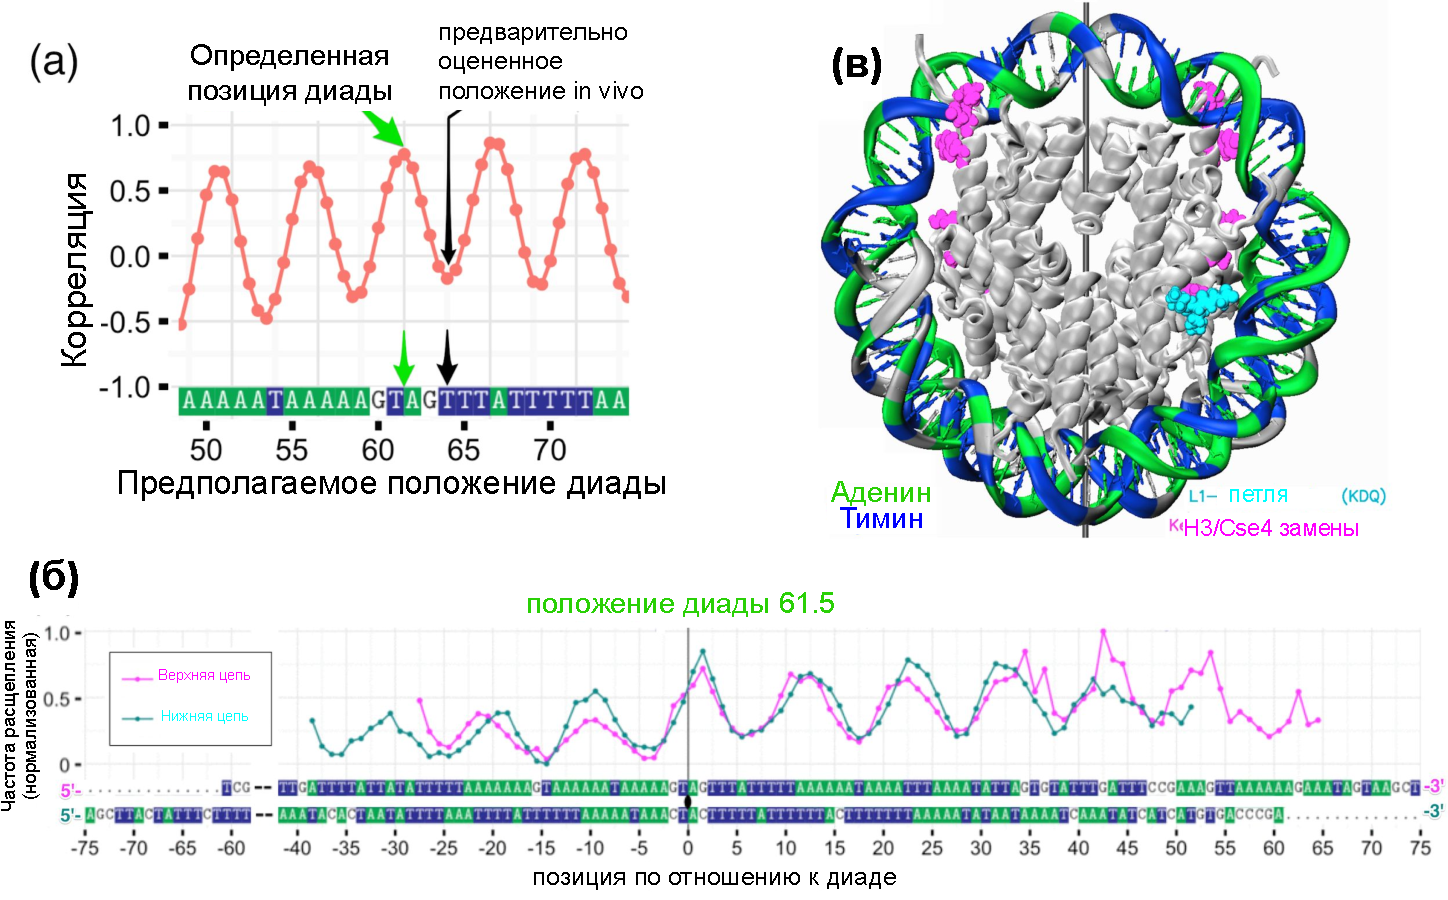
\includegraphics[width=\textwidth]{images/p5/part5_2_nar/p5_2_f8.pdf}
    \caption[Применение алгоритма идентификации диады  к нуклеосоме CEN3-NUC с неизвестным положением диады.]{Применение алгоритма идентификации диады к нуклеосоме CEN3-NUC с неизвестным положением диады. (A) коэффициент корреляции Пирсона между экспериментальными профилями расщепления верхней (TS) и нижней (BS) цепей ДНК как функция предполагаемого положения диады; зеленая стрелка - определенное положение, черная стрелка ранее предполагавшееся по \textit{in vivo} данным \cite{cole_centromeric_2011}. (Б) Наложение профилей TS и BS. (В) Полученная модель нуклеосомы (диада установлена в положение 61). Нити ДНК окрашены в соответствии с их последовательностью, выделяя AT-участки: A –– зеленый, T –– синий, G или C –– серый.}
    \label{fig:p5:p5_2_f8}
\end{figure}


\noindent
 которое обеспечивает выполнение вышеуказанного правила. Данный подход позволяет с точностью до одного нуклеотида определить позицию последовательности ДНК на нуклеосомном коре. С помощью данного подхода было определено ранее неизвестное положение ДНК в \textit{in vitro} модели центромерной нуклеосомы третьей хромосомы \textit{S. cerevisiae} (CEN3-NUC) и построена ее структурная модель (рис. \ref{fig:p5:p5_2_f8}). Обсуждается значение данной модели для понимания функционирования центромерных нуклеосом пекарских дрожжей, нуклеосомная ДНК которых содержит функционально важные последовательности аденинов (А-тракты). 





Материалы данной главы основаны на следующих статьях \cite{shaytan_hydroxyl-radical_2017,shaytan_structural_2018,armeev_modeling_2016}.

\textit{Выводы главы 3} \newline
Данные гидроксильного футпринтинга ДНК могут быть эффективно использованы для построения структурных моделей ДНК-белковых комплексов. Для ДНК-белковых комплексов, обладающих осью симметрии второго порядка, сравнение профилей расщепления ДНК для двух цепей позволяет дополнительно повысить точность определения положения ДНК относительно белка. 






Рассмотренный в третьей главе подход с учетом данных футпринтинга ДНК, позволяет определять с высокой точностью сайты взаимодействия ДНК с белками. Такой подход хорошо работает для определения положения ДНК на нуклеосомах, однако для построения моделей более сложных систем таких, как комплексы нуклеосом с белками хроматина, одних данных футпринтинга обычно не достаточно. В \underline{\textbf{четвертой главе}} \textit{(Моделирование комплексов нуклеосом с белками хроматина)} на конкретных примерах излагаются подходы по интегративному моделированию таких комплексов, в том числе с использованием разнородных экспериментальных данных низкого информационного содержания (футпринтинг ДНК, электронная микроскопия, FRET-микроскопия). Главу предваряет введение с описанием современных представлений о структуре хроматина и некоторых подходах к его моделированию.

\textit{Раздел 4.2} посвящен моделированию элонгационных комплексов РНК-полимеразы при транскрипции через нуклеосому на основе данных электронной микроскопии низкого разрешения и данных футпринтинга ДНК. Продвижение РНК-полимеразы вдоль ДНК является сложным биохимическим процессом (Рис. \ref{fig:p6_2_polII_synopsis}А), моделирование которого на данный момент лежит за пределами возможностей молекулярной динамики и квантовой химии, поэтому является хорошей задачей для применения интегративных методов.  Согласно экспериментальным данным при транскрипции РНК-полимеразой II через нуклеосому наблюдается ряд необычных фактов \cite{kulaeva_mechanism_2013}. Нуклеосомы зачастую ``выживают'' при транскрипции, то есть сохраняют свое положение на ДНК, что очень важно для сохранения разметки генома в виде эпигенетических пост-трансляционных модификаций гистонов. Предполагается, что выживание нуклеосом становится возможным благодаря образованию интермедиата ``нулевой'' петли в районе положения +49 после входа полимеразы в нуклеосому. В этом интермедиате ДНК за полимеразой восстанавливает контакты с октамером гистонов, таким образом, поддерживает его стабильность.
Структуры полимеразы и нуклеосомы известны по отдельности, однако каким образом образуется их комплекс при прохождении полимеразы через различные положения на нуклеосоме оставалось непонятным. С использованием представления геометрии ДНК в виде параметров взаимного расположения пар оснований нами был разработан подход по генерации ансамбля комплексов с различным положением полимеразы, а также возможностью варьировать уровень отворота ДНК от нуклеосомы. Данный подход, в том числе позволил связать ориентационное и трансляционное положение полимеразы и нуклеосомы в комплексе. Далее проводился анализ моделей на предмет оптимальной корреляции пространственного распределения атомов с экспериментальной электронной плотностью и отсутствия стерических перекрываний атомов в комплексе. В результате анализа выбиралась оптимальная модель.

% В большей степени это относится к тетрамеру гистонов H3/H4 тогда, как димеры гистонов H2A/H2B чаще уходят в раствор и заменяются. РНК полимераза испытывает паузирование как при входе в нуклеосому, так и в районе 40-50 нуклеотидов после входа в нуклеосому, что может играть важную роль в регуляции транскрипции, учитывая, что различные факторы (белки хроматина, шапероны гистонов, пост-трансляционные модификации и т.д.) могут влиять на это паузирование.

 Модель комплекса нулевой петли, построенная нами в совместных экспериментально-теоретических работах , представлена на рисунке \ref{fig:p6_2_polII_synopsis}В. Детальный анализ данных моделей позволил выдвинуть гипотезу о том, что ряд отрицательно заряженных областей РНК-полимеразы II способствует стабильности данного комплекса (рис. \ref{fig:p6_2_polII_synopsis}Г). Данные предположения подтверждаются сравнением моделей и экспериментальных данных для ряда бактериальных РНК-полимераз \cite{chang_analysis_2014}. Поскольку комплекс нулевой петли требует времени для образования, то пауза, возникающая при транскрипции, может приводить к откату (backtracking) активного центра полимеразы назад \cite{gaykalova_structural_2015}. Модель данного комплекса была также построена нами и представлена на рисунке \ref{fig:p6_2_polII_synopsis}Б.



\textit{Раздел 4.3} посвящен построению моделей разворачивания нуклеосом при их взаимодействии с комплексом гистоновых шаперонов FACT по данным экспериментов мономолекулярного FRET.
В данном случае по данным FRET были оценены расстояния между положениями ДНК, в которых  были введены флюоресцентные метки. К огрубленной физической модели ДНК (представленной в динуклеотидном приближении) добавлялся эмпирический гармонический потенциал, призванный свести расстояние между метками к наблюдаемому экспериментально. В результате оптимизации энергии были построены модели, в которых показаны возможные моды разворачивания ДНК и гистонов, удовлетворяющие экспериментальным данным \cite{valieva_large-scale_2016}.

В этой главе также изложены результаты анализа связывания центромерных нуклеосом пекарских дрожжей с белком внутренней кинетохоры Mif2 по данным гидроксильного футпринтинга. В главе 3 рассмотрена модель центромерной нуклеосомы и точно определено положении ДНК последовательности в ней. При анализе комплекса на профили доступности ДНК к расщеплению оказывало влияние взаимодействие ДНК не только с гистонами, но и с белком Mif2. Путем сравнения экспериментальных 



\begin{figure} [H]
    \centering
    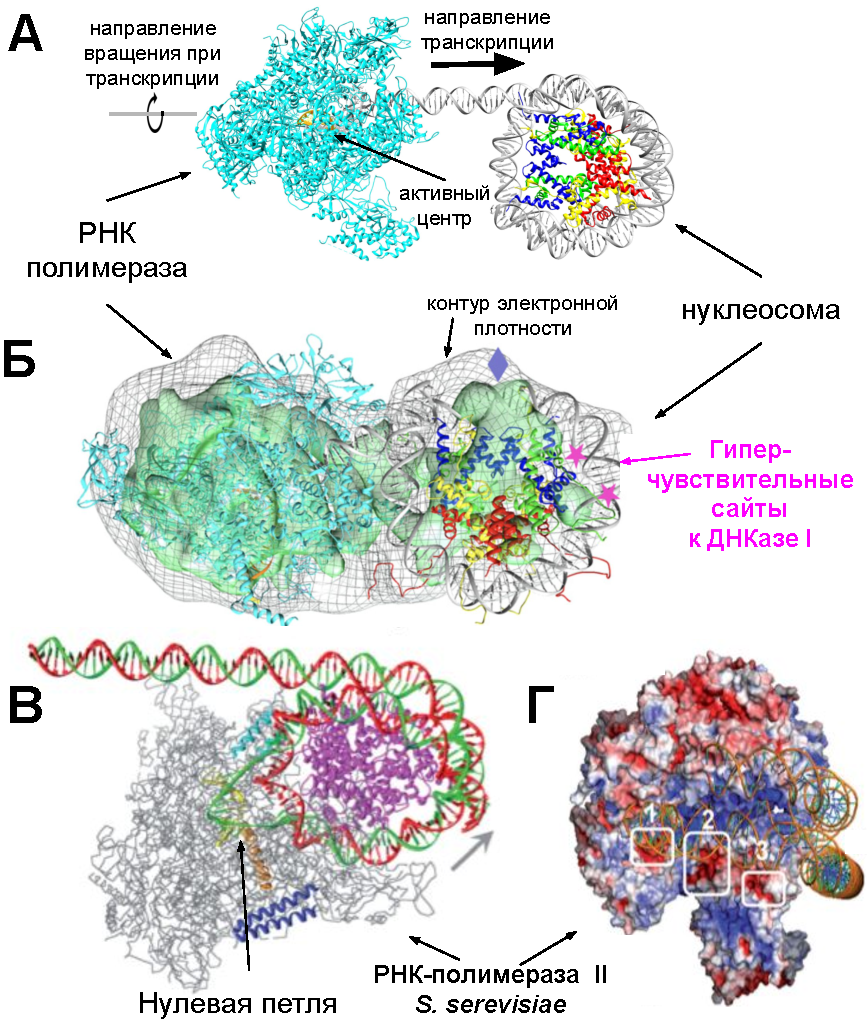
\includegraphics[width=\textwidth]{images/p6/p6_2/p6_2_polII_synopsis.pdf}
    \caption{Моделирование комплексов РНК-полимеразы (РНКП) и нуклеосомы. А. Принципиальная схема движения РНКП по ДНК к нуклеосоме. Б. Структура комплекса РНКП \textit{E. coli} с активным центром в положении +42 после входа в нуклеосому, построенная путем подбора оптимальной структуры комплекса, вписывающейся в электронную плотность и удовлетворяющая данным по доступности ДНК к расщеплению ДНКазе I \cite{gaykalova_structural_2015}. В. Модель комплекса в положении +49 (нулевая петля) с РНКП II \textit{S. cerevisiae} \cite{chang_analysis_2014}. Г. Поверхность полимеразы, взаимодействующая с нуклеосомой раскрашенная по заряду. Рамками обозначены отрицательно заряженные области предположительно стабилизирующие комплекс \cite{chang_analysis_2014}. }
    \label{fig:p6_2_polII_synopsis}
\end{figure}

\noindent
данных, обработанных с помощью разработанной программы HYDROID, было показано, что димер белка Mif2 взаимодействует с одной из сторон нуклеосомы в районе 5-35 пар нуклеотидов от центра нуклеосомы.   \cite{xiao_molecular_2017}. В главе также приводятся результаты по анализу комплексов нуклеосом с гистоном H1. 
Обсуждается результаты моделирования конформации линкерной ДНК при связывании гистона H1 по данным FRET, а также энергетические предпочтения изгиба линкерной ДНК при различных модах связывания гистона H1 \cite{gorkovets_joint_2018,bass_effect_2019,armeev_modeling_2016}. 

Материалы главы основаны на следующих статьях \cite{xiao_molecular_2017,gaykalova_structural_2015,valieva_large-scale_2016,gorkovets_joint_2018,bass_effect_2019,armeev_modeling_2016}.



\textit{Выводы главы 4} \newline
%В данной главе были изложены результаты по применению интегративных подходов для моделирования комплексов нуклеосом с белками хроматина. Изложены результаты работ, в которых были получены различные комплексы нуклеосом с РНК-полимеразой, конформации нуклеосом при связывании гистона H1 и комплекса FACT, модели взаимодействия нуклеосом с белком CENP-C. 
Автором продемонстрировано, что методы интегративного моделирования способны решать важный класс задач при изучении супрануклеосомной структуры хроматина, исследования которой затруднительны классическими методами структурной биологии, а именно создавать модели комплексов нуклеосом с белками хроматина на основе использования экспериментальных данных электронной микроскопии низкого разрешения, данных FRET-микроскопии, данных футпринтинга ДНК. Получены структурные и динамические модели различных комплексов, возникающих при взаимодействии нуклеосом с РНК-полимеразами, гистоном H1, комплексом FACT.





В \underline{\textbf{пятой главе}} (\textit{Интегративное моделирование амилоидоподобных фибрилл}) рассмотрены подходы к определению структуры фибриллярных комплексов, образующихся при самосборке олигопептидов. Задача заключается в определении формы комплекса и его внутренней организации.
В этом подходе экспериментальные данные используются уже на этапе конструирования возможных межмолекулярных укладок пептидов и на этапе оценки крупномасштабной морфологии фибрилл.

В начале главы дается подробный обзор литературы о свойствах и характеристиках амилоидных и амилоидоподобных фибрилл (в том числе конъюгированных с синтетическими молекулами), типах известной или предполагаемой их структурной организации. 
%Отдельно обсуждаются работы по использованию агрегационных свойств пептидов для создания самособирающихся нанотехнологических конструкций. В частности, дается обзор работ по конъюгатам синтетических полимеров с пептидами, приводятся экспериментальные данные по самосборке фибрилл на основе диблок олигомеров кватротиофен-пептид. Тифоены являются проводящими полимерами и поэтому такие системы рассматриваются с точки зрения создания самособирающихся ``нанопроводов''.

\textit{Раздел 5.2} посвящен работам по интегративному моделированию структуры амилоидоподобных фибрилл из диблок олигомеров тетратиофен-(Thr-Val)$_3$-пептид. Была разработана методология, позволяющая на основе ограниченного набора данных (ИК-, КД-спектроскопия, рентгеновская дифракция, данные атомно-силовой микроскопии, просвечивающей электронной микроскопии и т.д.) реконструировать наиболее вероятные атомистические модели и укладки молекул в фибриллах. Схема разработанной стратегии изображена на рисунке \ref{fig:p4_p5_f54}. Известно, что в основе амилоидных фибрилл  лежит укладка пептидов в $\beta$-листы.
%Однако конкретный тип такой укладки зачастую не известен. Он может включать как параллельные, так и антипараллельные $\beta$-листы, которые в свою очередь могут взаимодействовать различными сторонами. Изначальный отбор данных укладок может быть произведен с учетом данных ИК- и КД-спектроскопии, рентгеновской дифракции от фибрилл.
Данные спектроскопии могут помочь отличить наличие параллельных от анти-параллельных $\beta$-листов. Данные дифракции оценить периодичность укладки $\beta$-нитей в листе и $\beta$-листов относительно друг друга. Варианты укладки можно оценить на основе расчета энтальпии образования при моделировании укладок методом МД в растворителе и использовать для построения начальных моделей фибрилл. С использованием алгоритмов диссипативной динамики частиц можно определить крупномасштабную морфологию фибрилл (включая период кручения и персистентную длину) и сопоставить с данными микроскопии. На основе данного подхода было проведено комплексное исследование различных вариантов молекулярной организации фибрилл на основе олигомеров тиофен-пептид, определены наиболее вероятные модели, наблюдаемых в эксперименте фибрилл, в том числе на графите. Практической мотивацией создания такого рода фибрилл, являются проводящие свойства тиофена, что может приводить к формированию проводящих фибрилл ``нанопроводов''.  

\begin{figure} [H]
    \centering
    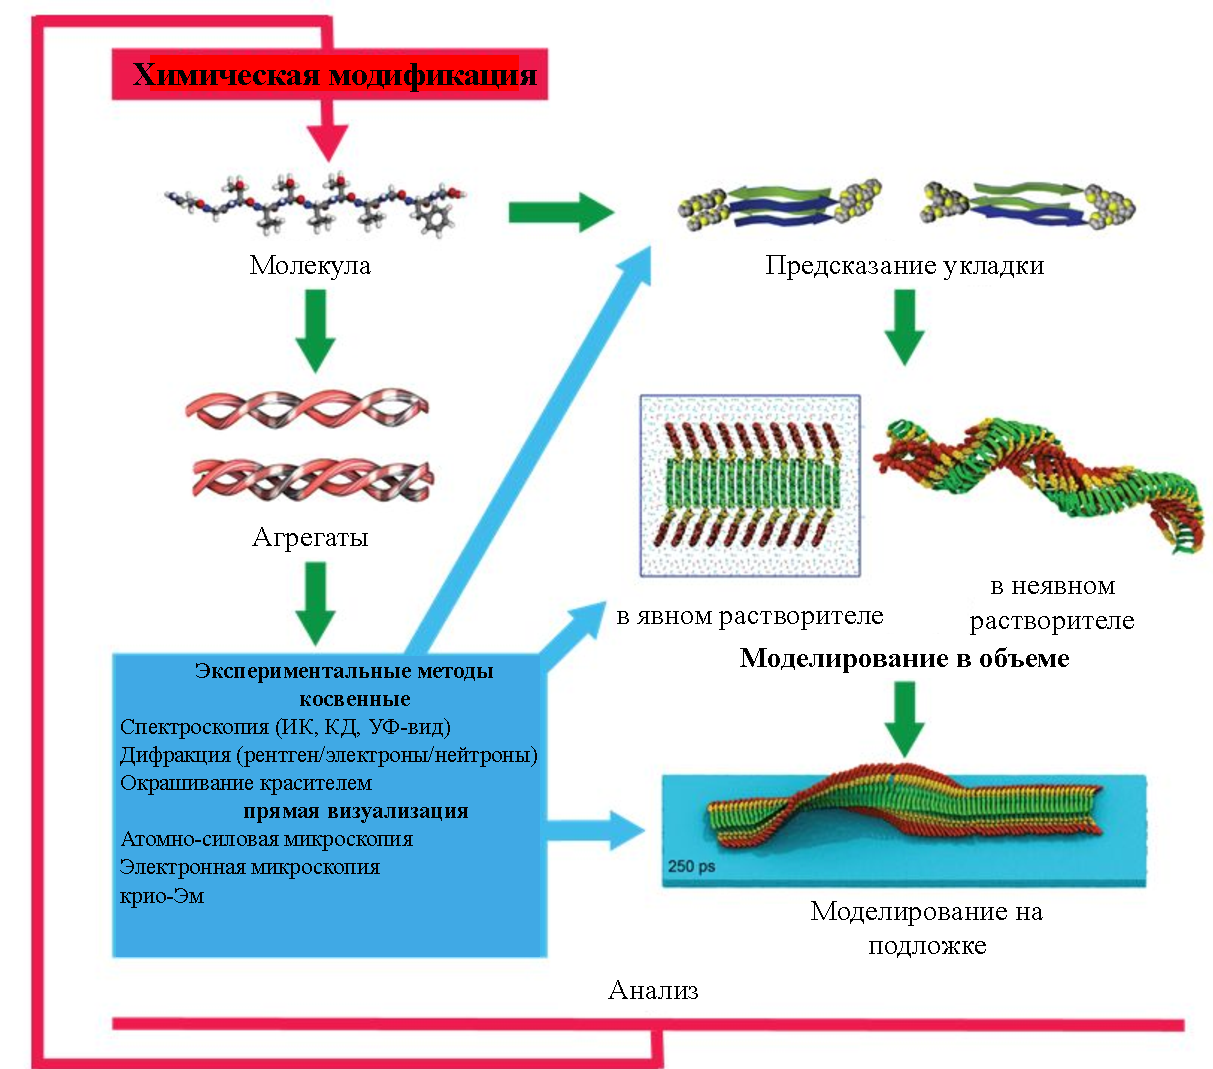
\includegraphics[width=\textwidth]{images/p4/punkt5/part4_p5_f54.pdf}
    \caption[Схематическое изображение комбинированной экспериментальной/вычислительной интегративной методологии для изучения амилоидоподобных фибрилл]{Схематическое изображение комбинированной экспериментальной/вычислительной интегративной методологии для изучения амилоидоподобных фибрилл.}
    \label{fig:p4_p5_f54}
\end{figure}


\textit{Раздел 5.3} посвящен применению разработанного подхода для установления молекулярной структуры пептидных амилоидоподобных фибрилл EF-C, образующихся из 12-аминокислотного пептида QCKIKQIINMWQ. Данные пептиды были выделены, как часть сиквенса гликопротеина gp120 ВИЧ-1. Экспериментально было установлено, что наличие данного пептида приводит к увеличению инфицирования клеток вирусом до 34 раз. На основе данных атомно-силовой микроскопии, кругового дихроизма, инфракрасной спектроскопии, порошковой дифракция рентгеновских лучей с применением разработанного нами интегративного подхода была построена молекулярная модель фибрилл EF-C (рис. \ref{fig:p4_nn2013_f2}г – e) \cite{yolamanova_peptide_2013}. Установлено, что боковые цепи лизина образуют гидрофильную поверхность с высокой плотностью катионных зарядов при физиологическом pH (рис. \ref{fig:p4_nn2013_f2}е)., таким образом усиливая проникновение генетического материала вируса в клетку.
    
   

\begin{figure} [H]
    \centering
    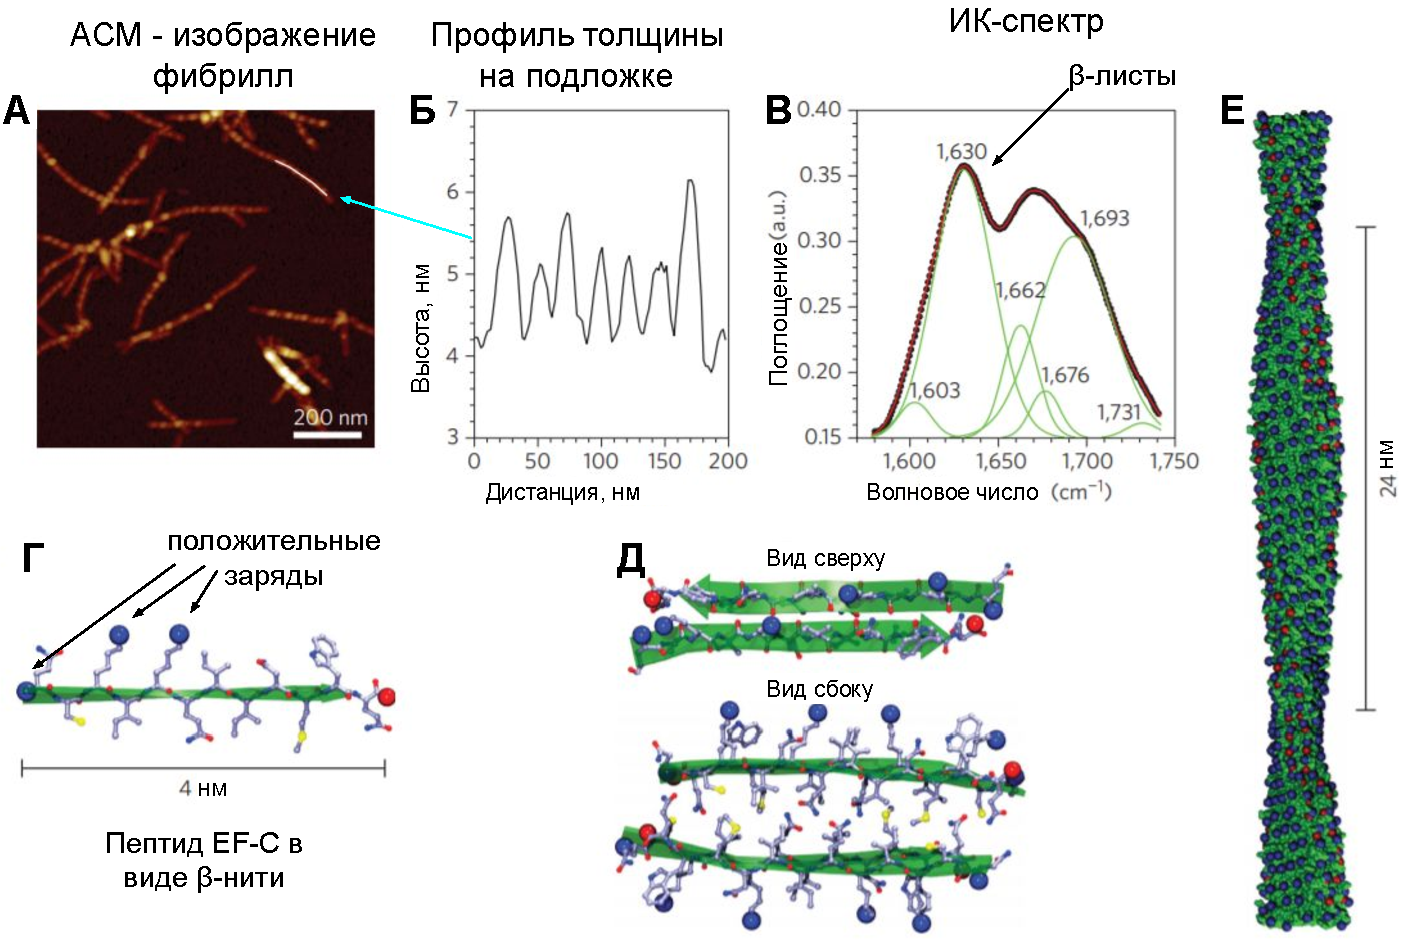
\includegraphics[width=\textwidth]{images/p4/natnanotech2013/nn2013/nn2013_f2.pdf}
    \caption[Структурная характеристика и молекулярное моделирование фибрилл EF-C]{Структурная характеристика и молекулярное моделирование фибрилл EF-C. \textbf{А} - АСМ-изображение фибрилл EF-C. \textbf{Б}, профиль по указанной линии в \textbf{А}. \textbf{В}, ИКФС-спектр, \textbf{Г} - Молекулярная модель пептида EF-C. \textbf{Д}, вид  сверху и сбоку элементарной единицы фибриллы, состоящей из четырех $\beta$-нитей, собранных в стопку из двух антипараллельных $\beta$-листов. \textbf{е}, Уточненная молекулярная модель фибриллы с шагом спирали 28 нм. Атомы C, серый; N, синий; О, красный; S, желтый.}
    \label{fig:p4_nn2013_f2}
\end{figure}


Материалы данной главы основаны на следующих ключевых статьях \cite{shaytan_self-assembling_2011,shaytan_self-organizing_2011,yolamanova_peptide_2013}. 


\textit{Выводы главы 5} \newline
Разработаны подходы интегративного моделирования амилоидоподобных фибрилл, позволяющие реконструировать укладку пептидов и морофологию фибрилл на основе сочетания экспериментальных данных ИК- и КД-спектроскопии, рентгеновской дифракции, электронной и атомно-силовой микроскопии.
%По результатам работы данной главы можно сделать следующие выводы:
 %\begin{itemize}
%\item Разработаны подходы интегративного моделирования амилоидоподобных фибрилл, основанные на использовании экспериментальных данных (рентгеновская дифракция на фибриллах, ИК- и КД-спектроскопия, окрашивание красителями) для конструирования возможных укладок пептидов в амилоидные фибриллы, использовании методов молекулярной динамики (в том числе с использованием элементов диссипативной динамики частиц) для установления крупномасштабной морфологии фибрилл с заданной укладкой и последующем сравнении модельных морфологий с экспериментальными данными (электронная микроскопия, атомно-силовая микроскопия).
%\item В рамках комплексного теоретико-экспериментального интегративного подхода охарактеризовано взаимное расположение бета нитей и крупномасштабная морфологии фибрилл, состоящих из олигомеров тиофена и пептидов (самособирающиеся биоорганические нанопровода). Получены атомистические модели фибрилл согласующиеся с экспериментальными данным. Модели фибрилл основаны на антипараллельной сборке $\beta$-листов из пептидов с последующим взаимодействием двух лент гидрофильными сторонами. Предложены стратегии улучшения проводимости самособирающихся фибрилл, основанные на использовании параллельной укладки $\beta$-листов, которая должна приводить к более плотному контакту проводящих тиофеновых групп.
%\item С помощью разработанного подхода построена структурная модель положительно заряженных фибрилл EF-C, которые могут использоваться для ускорения взаимодействия вирусных векторов с эукариотическими клетками в ходе трансдукции или генной терапии. Построенная модель согласуется с экспериментальными данными и основана на антипараллельной укладке пептидов в $\beta$-листы. Данная укладка дополнительно стабилизируется электростатическими взаимодействиями между заряженными концами пептидов.
%\end{itemize}




В \underline{\textbf{заключении}} приведено обсуждение результатов работы, рекомендации по их использованию и выводы, которые сформулированы ниже.

%\pdfbookmark{Заключение}{conclusions} 

%% Согласно ГОСТ Р 7.0.11-2011:
%% 5.3.3 В заключении диссертации излагают итоги выполненного исследования, рекомендации, перспективы дальнейшей разработки темы.
%% 9.2.3 В заключении автореферата диссертации излагают итоги данного исследования, рекомендации и перспективы дальнейшей разработки темы.


\ifdefined\DISSER  
\section*{Обсуждение результатов}
\addcontentsline{toc}{section}{Обсуждение результатов} 
\else 
\underline{\textbf{Обсуждение результатов}}
\pdfbookmark{Обсуждение результатов}{disc} 
\fi

Построение и анализ структурных моделей биомакромолекулярных комплексов имеет ключевое значение в изучении структурной организации биологических систем. В реализации этого подхода принципиальную роль играют методы компьютерного молекулярного моделирования. %Во-первых, это связано с тем, что любые экспериментальные данные о взаимном расположении молекул априори являются косвенными и требуют вычислительной интерпретации. Во-вторых, методы компьютерного молекулярного моделирования позволяют при построении и анализе моделей использовать знания и фундаментальные представления о взаимодействии атомов и молекул между собой, что может существенно дополнить экспериментальную информацию.
 В данной работе рассмотрены возможности методов молекулярного моделирования в построении и анализе больших ДНК-белковых комплексов и амилодоподобных фибрилл. В результате были разработаны новые интегративные методы моделирования для больших комплексов, для изучения свойств которых недостаточно стандартных.

 Одним из наиболее широкораспространенных и развитых методов молекулярного моделирования является метод молекулярной динамики (МД). Физические модели молекул в методе МД основаны на рассмотрении взаимодействий между атомами в приближении классической механики Ньютона. Согласно этому для биомолекул по некоторым правилам задается эмпирическая функция зависимости потенциальной энергии системы от координат атомов (так называемое силовое поле). Теоретически, при идеальной точности задания силового поля и неограниченных вычислительных возможностях метод МД может работать в режиме ``вычислительного микроскопа'', который воспроизводит реальные процессы структурообразования и взаимодействия биологических молекул. Однако на практике мы имеем дело лишь с некоторым приближенным описанием взаимодействий, построенным по аддитивному принципу. Кроме того мы ограничены во временах моделирования, что делает возможным исследование молекулярных систем лишь в ограниченной области конформационного пространства вблизи их стартовых конформаций. Современное развитие методов МД обычно представляет собой повторяющийся двухстадийный процесс, в котором вслед за совершенствованием вычислительных возможностей следует совершенствование силовых полей. Характерным примером здесь является совершенствование моделей ДНК. Так, силовые поля класса AMBER были изначально параметризованы для воспроизведения экспериментальной геометрии ДНК в наносекундном диапазоне, однако, в середине 2000-ых, оказалось, что при временах моделировании свыше 10 нс изменения торсионных углов остова ДНК приводят к неправильной геометрии ДНК, и поэтому силовое поле было усовершенствовано. Были изменены параметры силового поля, отвечающие за энергетические термы вращения торсионных углов в ДНК, что привело к сохранению правильной В-формы ДНК на доступных временах моделирования. В середине 2010-ых ситуация повторилась, когда стандартные времена моделирования увеличились до микросекундного масштаба, и силовое поле было вновь усовершенствовано. Аналогичные примеры можно привести и для силовых полей белков, воды и ионов. Кроме правильного воспроизведения равновесных параметров молекулярных систем, отдельным вопросом является качество воспроизведения их динамики. Здесь с точки зрения силового поля важным является воспроизведение правильного энергетического баланса (заселенности) между различными конформациями. Мы показали \cite{shaytan_free_2010}, что на больших временах моделирования начинают проявляться энтропийные эффекты, которые в случае белков приводят к излишней стабилизации структурных моделей. На практике при исследовании динамических процессов в биомакромолекулярных комплексах методами МД моделирования, необходимо оценить с одной стороны, в каких временных диапазонах МД модель адекватно описывает систему, а с другой стороны, в каких временных диапазонах возможно компьютерное воспроизведение функционально интересных конформационных перестроек. Результаты нашего моделирования на примере нуклеосом показывают, что современные методы МД позволяют создавать структурно-динамические модели ДНК-белковых комплексов без как-либо видимых артефактов по крайней мере на временах в десятки микросекунд. Свободная ДНК сохраняет конформацию, свойственную В-форме ДНК, ионное окружение является стабильным, глобулярные домены белка являются стабильными, а неупорядоченные домены сохраняют повышенную конформационную подвижность. В тоже время проведенный нами анализ динамики показал, что на временном диапазоне в пределах одной микросекунды наблюдаются такие процессы, как флуктуации формы свободных участков ДНК, конденсация неупорядоченных белковых доменов по поверхность ДНК, появления локальных конформационных возмущений в участках ДНК, связанных с белком. На временных масштабах порядка десятков микросекунд можно уже изучать диссоциацию/реассоциацию ДНК от белка в отдельных сайтах связывания, частичную диффузию неупорядоченных доменов вдоль поверхности ДНК. В то же время, более крупномасштабные перестройки ДНК-белковых комплексов пока находятся за пределами возможностей МД. Так, вероятно, процессы комплексообразования, например, связывания транскрипционных факторов и поиск ими сайтов на последовательности ДНК или процессы образования гетероструктур ДНК-РНК (например, при связывании комплексов системы CRISPR-Cas9) находятся за пределами возможностей МД. Аналогичная ситуация возникает и при моделировании самосборки амилоидоподобных фибрилл. Несмотря на высокую точность задания силовых полей белков по сравнению с силовыми полями нуклеиновых кислот, ситуация здесь усложняется повышенными требованиями к точности определения энергии для различных конформаций пептидов. Известно, что амилоидоподобные фибриллы обладают конформационным полиморфизмом и в экспериментальных работах небольшое изменение условий (состав растворителя, температура) и, соответственно, энергетического баланса может приводить к формированию фибрилл различного типа. 

Именно для решения такого рода задач, мы обратились к развитию и разработке методов интегративного моделирования. Базовая идея разработанных методов интегративного моделирования состоит в объединении информации заложенной в силовых полях с информацией о взаимном расположении элементов структуры, которую мы получаем из дополнительных экспериментальных методов.
Общая логика построения интегративных подходов может быть сформулирована следующим образом. При моделировании структурных элементов и параметров системы, на структуру и значения которых  может сильно повлиять неточность силовых полей, необходимо дополнительно привлекать экспериментальные данные. Вместе с тем, моделирование конформационно устойчивых структурных элементов можно производить на основании данных силовых полей. Примером служат полученные результаты моделирования комплексов нуклеосом с РНК полимеразой или моделирования геометрии линкерной ДНК при связывании гистона H1. Предполагалось, что свободная ДНК в целом должна находится в В-конформации двойной спирали, согласно параметрам, заложенным в силовом поле, описывающем структуру ДНК. В то же время более тонкие параметры, такие как небольшой изгиб ДНК, уровень ее отворота от нуклеосомы определяются ограничениями, накладываемыми согласно дополнительными экспериментальными данными. 
В целом аналогичной логике мы следовали при интегративном моделировании амилоидоподобных фибрилл. Были выделены параметры, которые сложно воспроизвести только с помощью моделирования, а именно, параметры укладки пептидов внутри фибриллы, и параметры, которые воспроизводятся моделированием с хорошей точностью, а именно, связь морфологии фибриллы с межмолекулярной укладкой пептидов. Таким образом, экспериментальные данные использовались частично при выборе укладок, а также для отбора фибрилл на уровне их крупномасштабной морфологии.

Таким образом общий принцип разработки интегративных подходов различных биомакромолекулярных комплексов, который можно рекомендовать, состоит в следующем. В первую очередь с учетом известных экспериментальных и литературных данных проводится анализ различных уровней структурной организации моделируемой системы, выделяются уровни организации, моделирование которых эффективно может быть проведено на основе имеющихся силовых полей, а также уровни организации, при моделировании которых необходимо привлекать дополнительные экспериментальные данные. На следующем этапе необходимо использовать различные интегративные методы моделирования, которые позволяют одновременно учитывать как различные экспериментальные данные, так и данные основанные на представлениях о внутримолекулярной структуре и межмолекулярных взаимодействиях. 

В интегративном моделировании весьма полезным походом является использования соображений структурной симметрии. В некоторых случаях они позволяют кардинальным образом упростить задачу, повысить точность моделирования и уменьшить влияние возможных систематических ошибок в экспериментальных данных. Именно этот подход был продемонстрирован при использовании данных футпринтинга ДНК в построении моделей нуклеосом. На качество профиля футпринтинга вдоль нити ДНК могут оказывать влияние такие факторы, как наличие минорных альтернативных продуктов химического расщепления, локальная динамика ДНК в процессе реакции, шумовой фон. Однако, в силу наличия оси симметрии второго порядка в нуклеосоме такие эффекты будут симметричны для двух цепей ДНК и не влияют на алгоритм поиска положения в ДНК, относительно которого профили симметричны. Аналогичные соображения можно рекомендовать использовать при интегративном моделировании других ДНК белковых систем, обладающих симметрией. К таким системам относятся многие транскрипционные факторы, формирующие гомодимеры. 


\underline{\textbf{Заключение}}
\ifdefined\DISSER   \else \pdfbookmark{Заключение}{conclusion} \fi

В настоящей работе автором развиты новые системные подходы для построения структурно-динамических моделей сложных биомакромолекулярных комплексов. Разработанные интегративные методы молекулярного моделирования основаны на сочетании (интеграции) физических моделей взаимодействия молекул с информацией получаемой из различных источников экспериментальных данных. В ходе исследования развиты подходы, (i) позволяющие проводить анализ динамики атомистических структур в микросекундном временном диапазоне, (ii) учитывать различные экспериментальные данные при построении моделей (например, данные экспериментов по футпринтингу ДНК, данные электронной микроскопии, данные FRET-микроскопии, данные рентгеновской дифракции на фибриллах, атомно-силовой микроскопии и т.д.), (iii) сочетать атомистическое и огрубленное представление молекулярных систем (в частности при моделировании ДНК-содержащих комплексов).


Разработанные автором подходы и методы рекомендуется применять для установления структуры и динамической подвижности биомакромолекулярных комплексов, размер и свойства которых затрудняют применение стандартных методов структурной биологии. Практическое применение данных подходов продемонстрировано в диссертации на примере ряда биомакромолекулярных систем, в том числе нуклеосом, комплексов нуклеосом с белками хроматина, амилоидоподобных фибрилл.



\ifdefined\DISSER  
\section*{Выводы диссертационной работы}
\addcontentsline{toc}{section}{Выводы диссертационной работы} 
\else 
\underline{\textbf{Выводы диссертационной работы}}
\pdfbookmark{Выводы диссертационной работы}{vivodi}
\fi

\begin{enumerate}
  %\item Разработаны подходы и программные решения для мультимасштабного моделирования комплексов ДНК и белков с использованием информации из экспериментов по ДНК футпринтингу, электронной микроскопии, FRET-микроскопии. Комбинированное представление ДНК как в атомистическом, так и в динуклеотидном приближении позволяет проводить быструю крупномасштабную оптимизацию структур и при этом учитывать атомистические детали взаимодействия ДНК с белками.
\item Разработан интегративный подход и программные решения для мультимасштабного моделирования комплексов ДНК и белков, в котором используются различные данные экспериментов по ДНК футпринтингу, электронной микроскопии, FRET-микроскопии и комбинированное представление ДНК в атомистическом и в динуклеотидном приближении.

  % \item Разработанные подходы суперкомпьютерного моделирования нуклеосом позволили изучить динамические характеристики нуклеосом в микросекундном временном диапазоне. Охарактеризованы крупномасштабные функциональные конформационные изменения - флуктуации линкерной  ДНК, диссоциация ДНК от гистонового октамера, образование дефектов кручения ДНК, переключения конформаций гистоновых хвостов.

  \item В микросекундном временном диапазоне определены параметры крупномасштабных функциональных конформационных изменений структуры нуклеосом: вычислен ансамбль конформаций линкерной ДНК, установлено влияние электростатического отталкивания на геометрию сегментов линкерной ДНК, определено характерное время диссоциации концов нуклеосомальной ДНК от гистонового октамера (10 мкс), установлены флуктуационные структурные механизмы образования дефектов кручения ДНК, переключения конформаций гистоновых хвостов.

  %\item Cовременные методы суперкомпьютерной атомистической молекулярной динамики позволяют рассчитывать для малых молекул на основе заданной модели атом-атомных взаимодействий термодинамические параметры гидратации (свободную энергию гидратации и адсорбции) с высокой статистической точностью (ошибка 1 kT и меньше в зависимости от длины расчета). Расчет профилей свободной энергии боковых цепей аминокислот вблизи поверхности воды указывает на наличие минимума свободной энергии на поверхности воды (вблизи участка, где плотность равна половине от объемной плотности). 

  

  \item Обработка экспериментальных данных по расщеплению ДНК гидроксильными радикалами (футпринтинга ДНК) позволила вычислить вероятность расщепления ДНК для каждого нуклеотида. Показано, что профили расщепления ДНК гидроксильными радикалами в нуклеосоме мало зависят от последовательности ДНК, и определяются в основном позиционированием ДНК на нуклеосоме. Предложен алгоритм точного определения положения ДНК в нуклеосоме по данным футпринтинга для двух цепей ДНК на основании положения оси псевдосимметрии.

  \item С помощью методов интегративного моделирования были установлены структуры и параметры взаимодействий комплексов нуклеосом с РНК полимеразами, белком CENP-C, гистоном H1, белками комплекса FACT. Установлено, что в положении +49 после входа в нуклеосому РНК полимераза II может формировать компактный комплекс с нуклеосомой, в котором контакты гистонов с ДНК сохраняются по обе стороны активного центра. В модели центромерной нуклеосомы дрожжей определено положение ДНК и установлено, что белок CENP-C взаимодействует с нуклеосомой в районе 20 нуклеотидов от центра симметрии нуклеосомы. Предложены модели конформации линкерных сегментов ДНК при связывании гистона H1.  Установлены амплитуды конформационной подвижности ДНК в нуклеосомах при связывании с комплексом FACT.
  
  %модели указывают на то, что конформационно-динамический полиморфизм нуклеосом является важным фактором при их взаимодействии с белками хроматина. Структура нуклеосом может серьезным образом изменяется при взаимодействиях с белками хроматина (например, в изученном нами взаимодействии с комплексом FACT). Структура комплексов нуклеосом с белками хроматина также зачастую зависит от деталей их состава и внешних условий (например, продемонстрировано нами при моделировании полиморфизма связывания нуклеосомы с гистоном H1). Структура и ориентация ДНК на нуклеосоме является важным фактором для узнавания белками хроматина, что продемонстрировано в работах по изучению комплексов CENP-C с нуклеосомой.

 \item Разработанные подходы построения моделей амилоидоподобных фибрилл позволили изучить связь взаимного расположения пептидов в фибриллярных структурах с крупномасштабной морфологией амилоидоподобных фибрилл и таким образом установить структурную организацию филаментов на основе диблок олигомеров кватертиофена и пептида $(Thr-Val)_3$, а также на основе фрагмента белка gp120. Установлено, что рассмотренные амилоидоподобные фибриллы могут образовываться на основе двух взаимодействующих бета-листов, которые формируют либо плоскую ленту, либо левозакрученную ленту с периодом 24-30 нм.

\end{enumerate}




\medskip
\pdfbookmark{Основные публикации автора по теме диссертации}{authorbibliography} 
\textbf{Основные публикации Шайтана Алексея Константиновича по теме диссертации в рецензируемых научных изданиях, индексируемых в базах данных Web of Science, Scopus, RSCI, рекомендованных для защиты в диссертационном совете МГУ по специальности 03.01.09 - <<Математическая биология, биоинформатика>>}\footnote{В скобках приведен объем публикации в печатных листах и вклад автора в печатных листах.}
\ifdefmacro{\microtypesetup}{\microtypesetup{protrusion=false}}{} % не рекомендуется применять пакет микротипографики к автоматически генерируемому списку литературы
\urlstyle{rm}                               % ссылки URL обычным шрифтом
\ifnumequal{\value{bibliosel}}{0}{% Встроенная реализация с загрузкой файла через движок bibtex8
  \renewcommand{\bibname}{\large \bibtitleauthor}
  \nocite{*}
  \insertbiblioauthor           % Подключаем Bib-базы
  %\insertbiblioexternal   % !!! bibtex не умеет работать с несколькими библиографиями !!!
}{% Реализация пакетом biblatex через движок biber
  % Цитирования.
  %  * Порядок перечисления определяет порядок в библиографии (только внутри подраздела, если `\insertbiblioauthorgrouped`).
  %  * Если не соблюдать порядок "как для \printbibliography", нумерация в `\insertbiblioauthor` будет кривой.
  %  * Если цитировать каждый источник отдельной командой --- найти некоторые ошибки будет проще.
  %
  %перенесено наверх
  %\nocite{
        %high impact in right order (do not remove or change)
        %64 статьи и тезисы + 2 диссертации (тут не учитываются)
        %VAK изданий 56, не вак 8, тезисов 17, статей 47
        %NB no of these should appear in othercites.bib (!) - they will then disappear from author list of papers
   %    armeev_linking_2019,hada_histone_2019,shaytan_structural_2018,shaytan_hydroxyl-radical_2017,xiao_molecular_2017,draizen_histonedb_2016,el_kennani_ms_histonedb_2017,shaytan_coupling_2016,valieva_large-scale_2016,gaykalova_structural_2015,frank_direct_2015,nishi_physicochemical_2014,yolamanova_peptide_2013,shaytan_self-assembling_2011,shaytan_self-organizing_2011,shaytan_large-scale_2010,shaytan_free_2010,shaytan_solvent_2009,kasimova_voltage-gated_2014,chang_analysis_2014,sokolova_genome_2014,%=======
    %      armeev_analyzing_2019,armeev_conformational_2015,armeev_integrative_2020,kniazeva_analyzing_2020,armeev_linking_2019,armeev_modeling_2016,armeev_molecular_2015,armeev_nucleosome_2016,armeev_python_2019,bass_effect_2019,biswas_genomic_2016,bozdaganyan_comparative_2014,chang_analysis_2014,chang_pausing_2013,chang_structural_2013,chertkov_dual_2017,draizen_histonedb_2016,el_kennani_ms_histonedb_2017,frank_direct_2015,gaykalova_structural_2015,goncearenco_structural_2015,gorkovets_joint_2018,gorkovets_mutual_2018,gribkova_construction_2019,gribkova_investigation_2017,hada_histone_2019,kasimova_investigation_2014,kasimova_molecular_2014,kasimova_voltage-gated_2014,levtsova_molecular_2009,lyubitelev_structure_2016,nikolaev_dynamics_2010,nikolaev_vzaimodeistvie_2010,nishi_physicochemical_2014,orekhov_calculation_2012,shaitan_dynamics_2016,shaitan_influence_2013,shaytan_combined_2015,shaytan_coupling_2016,shaytan_free_2010,shaytan_hydroxyl-radical_2017,shaytan_large-scale_2010,shaytan_microsecond_2017,shaytan_molekularnaya_2005,shaytan_neravnovesnaya_2006,shaytan_nucleosome_2015,shaytan_nucleosome_2016,shaytan_polymorphism_2015,shaytan_self-assembling_2011,shaytan_self-organizing_2011,shaytan_solvent_2009,shaytan_structural_2018,shaytan_trajectories_2016,sokolova_genome_2014,valieva_large-scale_2016,xiao_molecular_2017,yolamanova_peptide_2013,%далее диссертации
     %     shaytan_thesis_kfmn_2010,shaytan_thesis_ulm_2012,%не вак
      %    armeev_abstract_2019,armeev_modelirovanie_2013,bass_abstract_2019,greshnova_sinteticheskaya_2019,shaytan_dinamicheskiy_2006,shaytan_peptide_2006,shaytan_supercomputernoe_2009,shaytan_water_2014,%патенты
       %   patbib1,progbib1}
  %% authorvak
  %\nocite{vakbib1}%
 % \nocite{vakbib2}%
  %
  %% authorwos
 % \nocite{wosbib1}%
  %
  %% authorscopus
 % \nocite{scbib1}%
  %
  %% authorpathent
  %\nocite{patbib1}%
  %
  %% authorprogram
  %\nocite{progbib1}%
  %
  %% authorconf
  %\nocite{confbib1}%
 % \nocite{confbib2}%
  %
  %% authorother
  %\nocite{bib1}%
  %\nocite{bib2}%

  \ifnumgreater{\value{usefootcite}}{0}{
    \begin{refcontext}[labelprefix={}]
      \ifnum \value{bibgrouped}>0
        \insertbiblioauthorgrouped    % Вывод всех работ автора, сгруппированных по источникам
      \else
        \insertbiblioauthor      % Вывод всех работ автора
      \fi
    \end{refcontext}
  }{
  \ifnum \totvalue{citeexternal}>0
    \begin{refcontext}[labelprefix=*]
      \ifnum \value{bibgrouped}>0
        \insertbiblioauthorgrouped    % Вывод всех работ автора, сгруппированных по источникам
      \else
        \insertbiblioauthor      % Вывод всех работ автора
      \fi
    \end{refcontext}
  \else
    \ifnum \value{bibgrouped}>0
      \insertbiblioauthorgrouped    % Вывод всех работ автора, сгруппированных по источникам
    \else
      \insertbiblioauthor      % Вывод всех работ автора
    \fi
  \fi
  %  \insertbiblioauthorimportant  % Вывод наиболее значимых работ автора (определяется в файле characteristic во второй section)

\textbf{Зарегистрированные патенты и программы}

\begin{enumerate}
  \item Заявка 2580006 Рос. федерация, МПК G 06 F 19/100. Способ скрининга потенциальных противоопухолевых препаратов ингибиторов FACT [Текст] / В. М. Студитский, О. И. Студитская, А. К. Шайтан (Российская Федерация). — No 2013132806/10 ; заявл. 16.07.2013 ; опубл. 27.01.2015, Бюл. No 3 ; приоритет 16.07.2013 (Рос. Федерация). — 10 с.
\item Свидетельство о гос. регистрации программы для ЭВМ. Программный комплекс реконструкции пространственной структуры белков и комплексов на основе карт электронной плотности низкого разрешения [Текст] / Д. Л. Шуров, А. К. Шайтан, Г. А. Армеев, Д. А. Турченков, В. Н. Блинов, М. П. Кирпичников, К. В. Шайтан. — No 2013614397 ; заявл. 13.05.2013 ; опубл. 17.07.2013, 2013614397 (Рос. Федерация).
\end{enumerate}

  \pdfbookmark{Список литературы}{bibliography}
  \begin{refcontext}[labelprefix={}]
      \insertbiblioexternal            % Вывод списка литературы, на которую ссылались в тексте автореферата
  \end{refcontext}
  % Невидимый библиографический список для подсчёта количества внешних публикаций
  % Используется, чтобы убрать приставку "А" у работ автора, если в автореферате нет
  % цитирований внешних источников.
  \printbibliography[heading=nobibheading, section=0, env=countexternal, keyword=biblioexternal, resetnumbers=true]%
  }
}
\ifdefmacro{\microtypesetup}{\microtypesetup{protrusion=true}}{}
\urlstyle{tt}                               % возвращаем установки шрифта ссылок URL
